\chapter{Maximum Likelihood Estimation}\label{chap:ML}

In this chapter we begin the study of the estimation methods for spatial models. In particular, we focus in the maximum likelihood estimation method. However, it is important to know some basic of the different estimation methods. 

Spatial econometric models can be estimated by maximum likelihood (ML) \citep{ord1975estimation}, quasi-maximum likelihood (QML) \citep{lee2004asymptotic}, instrumental variables (IV) \citep[][pp. 82-86]{anselin1988spatial}, generalized method of moments (GMM) \citep{kelejian1998generalized, kelejian1999generalized}, or by Bayesian Markov Chain Monte Carlo method (Bayesian MCMC) \citep{lesage1997bayesian}.

As we will see in this chapter, the main drawback of the ML estimation is the assumption of normality of the error terms. QML and IV/GMM have the advantage that they do not rely on the assumption of normality of the disturbances. However, both estimators assume that the disturbance terms are independently and identically distributed for all $i$ with zero mean and variance $\sigma^2$.  IV/GMM estimator has the disadvantage that the estimate for $\rho$ or $\lambda$ may be out of the parameter space. These coefficients are restricted to the interval $(1/r_{\mbox{min}})$ by the Jacobian term in the ML estimation. This issue motivated the development of the IV/GMM, which do not require the Jacobian term.To instrument the spatially lagged dependent variable, Kelejian et al. (2004) suggest $\left[\mX, \mW\mX,...,\mW^g\mX\right]$, where $g$ is a pre-selected constant. 


%*********************************************************
%\section{ML}
%*********************************************************

%Given the econometric model $\vy = \mX\vbeta + \vepsi$, suppose that the vector $\vepsi$ follows a Normal distribution such that the mean is $\vzeros_n$ and variance-covariance matrix $\sigma^2\mI_n$. Given these hypothesis, the density function of vector $\vepsi$ is:


%\begin{eqnarray}
%	f(\vepsi) &=& \frac{1}{(2\pi)^{N/2}}\frac{1}{\left|\sigma^2\mI_n\right|^{1/2}}\exp\left[-\frac{1}{2}\vepsi^\top\left(\sigma^2\mI_n\right)^{-1}\vepsi\right] \nonumber \\
%	 &=& \frac{1}{(2\pi)^{N/2}}\frac{1}{\left(\sigma^2\right)^{1/2}}\exp\left[-\frac{1}{2\sigma^2}\vepsi^\top\vepsi\right]\label{eq:OLS_L}
%\end{eqnarray}

%The previous density function can be transformed into a sampling ML function if we express the vector $\vepsi$ as a function of the data. To do so we have to consider the transformation of variable Theorem \ref{teo:Transformation_var}. The jacobian that converts the random vector $\vepsi$ into the random vector $\vy$ is


%\begin{equation*}
%\begin{pmatrix}
%\frac{\partial \vepsi}{\partial \vy}
%\end{pmatrix} = \begin{pmatrix}
%\frac{\partial \epsilon_1}{\partial y_1} & \frac{\partial \epsilon_1}{\partial y_2} & \hdots & \frac{\partial \epsilon_1}{\partial y_n} \\
%\frac{\partial \epsilon_2}{\partial y_1} & \frac{\partial \epsilon_2}{\partial y_2} & \hdots & \frac{\partial \epsilon_2}{\partial y_n} \\
%\hdots & \hdots & \hdots & \hdots \\
%\frac{\partial \epsilon_N}{\partial y_1} & \frac{\partial \epsilon_N}{\partial y_2} & \hdots & \frac{\partial \epsilon_N}{\partial y_n}
%\end{pmatrix}=
%\begin{pmatrix}
%1 & 0 & 0 & \hdots & 0 \\
%0 & 1 & 0 & \hdots & 0 \\
%\hdots & \hdots & \hdots & \hdots \\
%0 & 0 & 0 & \hdots & 1 
%\end{pmatrix}
%\end{equation*}

%whose determinant is the unity. As a consequence, the ML function is obtained substituting into (\ref{eq:OLS_L}) the vector $\vepsi$ as a function of $\vy$, to get


%\begin{equation}
%L(\vy, \mX; \vbeta, \sigma^2)= (2\pi \cdot\sigma^2)^{-N/2}\exp\left[-\frac{1}{2\sigma^2}(\vy-\mX\vbeta)^\top (\vy-\mX\vbeta)\right]
%\end{equation}

%Note that $\mSigma = \sigma^2\mI$, $\left|\mSigma\right|^{-1/2} = \sigma^n$, $\mSigma^{-1} = \frac{1}{\sigma^2}\mI$, and $\left|\mSigma\right| = \left|\sigma^2\mI\right|=\sigma^{2n}$


%*********************************************************
\section{What Are The Consequences of Applying OLS?}\label{sec:consequences_slm}
%*********************************************************

We start this chapter analyzing the consequences of applying OLS model on a sample that follows a SAR process. The main result is that the estimated coefficients will be biased and inconsistent. This means that the estimated parameters will not be close to the true parameters, even if you have a very large data set, which is a serious problem.

%-----------------------------------------------
\subsection{Finite and Asymptotic Properties}
%-----------------------------------------------

First, we will show that an OLS estimate of $\rho$ will be biased under the SLM. To do so, and not get lost with the notation, consider the following pure first order spatial autoregressive model:

\begin{equation}\label{eq:simply_lag}
\underset{(n\times 1)}{\vy} = \rho_0\underset{(n\times 1)}{\mW\vy} + \underset{(n\times 1)}{\vepsi},
\end{equation}
%
where $\rho_0$ is the true population parameter of the data generating process (DGP). The reduced form for the \textbf{pure SLM} in (\ref{eq:simply_lag}) is:

\begin{equation}\label{eq:reduced_form_pure_slm}
\vy =\left(\mI_n - \rho_0\mW\right)^{-1}\vepsi.
\end{equation}

As a result, the spatial lag term equals:

\begin{equation}\label{eq:wy_pure}
  \mW\vy = \mW\left(\mI_n - \rho_0\mW\right)^{-1}\vepsi.
\end{equation}

This result will be useful later. Now, recall that if the model is $\vy = \mX\vbeta + \vepsi$, then the OLS estimator is $\widehat{\vbeta} = \left(\mX^\top\mX\right)^{-1}\mX^\top\vy$. Then, considering (\ref{eq:simply_lag}) the OLS estimator for $\rho_0$ is: 

\begin{equation}\label{eq:rho_ols}
\widehat{\rho}_{OLS} = \left[\underbrace{\left(\mW\vy \right)^\top}_{(1\times n)}\underbrace{\left(\mW\vy \right)}_{(n\times 1)}\right]^{-1}\underbrace{\left(\mW\vy \right)^\top}_{(1\times n)}\underbrace{\vy}_{(n\times 1)}.
\end{equation}

Substituting the expression for $\vy$ from the population Equation (\ref{eq:simply_lag}) into Equation (\ref{eq:rho_ols}) gives us the following sampling error equation:

\begin{equation*}
  \begin{aligned}
          \widehat{\rho}_{OLS} & = \rho_0 + \left[\left(\mW\vy \right)^\top\left(\mW\vy \right)\right]^{-1}\left(\mW\vy \right)^\top\vepsi \\
                               & = \rho_0 + \left(\sum_{i = 1}^n \vy_{Li}^2\right)^{-1}\left(\sum_{i = 1}^{n}\vy_{Li}\epsilon_i\right),
  \end{aligned}
\end{equation*}
%
where $\vy_{Li}$ is the $i$th element of the spatial lag operator $\mW\vy = \vy_L$. Assuming that $\mW$ is nonstochastic, the mathematical expectation of $\widehat{\rho}_{OLS}$ is

\begin{equation}\label{eq:expectation_of_pureslm}
  \begin{aligned}
\E\left(\left.\widehat{\rho}_{OLS}\right| \mW\right) & = \rho_0 + \E\left(\left.\left[\left(\mW\vy \right)^\top\left(\mW\vy \right)\right]^{-1}\left(\mW\vy \right)^\top\vepsi\right| \mW \right) \\
                         & = \rho_0 + \left(\sum_{i = 1}^n \vy_{Li}^2\right)^{-1}\E\left(\left.\sum_{i = 1}^{n}\vy_{Li}\epsilon_i\right| \mW\right).
  \end{aligned}
\end{equation}

From (\ref{eq:expectation_of_pureslm}) it is clear that if the expectation of the last term is zero, then $\widehat{\rho}_{OLS}$ will be unbiased. However, note that

\begin{equation}\label{eq:Eyle}
  \begin{aligned}
      \E\left(\left.\sum_{i = 1}^{n}\vy_{Li}\epsilon_i \right| \mW\right) & =  \E\left[\left.\left(\mW\vy \right)^\top\vepsi\right| \mW\right] \\
      & =  \E\left[\left.\underset{(1\times 1)}{\vepsi^\top \left( \mI -\rho \mW^\top\right)^{-1}\mW^\top\vepsi} \right| \mW \right] \quad \mbox{using (\ref{eq:wy_pure})}\\
      & =  \E\left[\left.\vepsi^\top \mC^\top \vepsi \right| \mW\right] \\
      & = \E\left[\left.\tr \vepsi^\top  \mC^\top\vepsi\right|\mW \right] \\
      & = \E\left[\left.\tr \mC^\top \vepsi\vepsi^\top\right| \mW\right] \\
      & =  \tr \left(\mC\right) \E\left(\left.\vepsi\vepsi^\top\right| \mW\right)\quad \mbox{since $\tr(\mA) = \tr(\mA^\top)$} \\
      & \neq 0,
  \end{aligned}
\end{equation}
%
where $\mC = \mW\left( \mI -\rho \mW\right)^{-1}$. Therefore, given the result in (\ref{eq:Eyle}) we have that $\E\left(\left.\widehat{\rho}_{OLS}\right| \mW\right) = \rho_0$ if and only if $\tr \left(\mC\right) = 0$, which occurs if $\rho_0 = 0$. If $\rho = 0$, $\mC = \mW$, and $\tr(\mC) = \tr(\mW) = 0$ because the diagonal elements of $\mW$ are zeros (See Definition \ref{definition:trace} for properties of the trace).  In other words, if the true model follows a spatial autoregressive structure, the OLS estimate of $\rho$ will be biased. 

\begin{definition}[Some useful results on trace]\label{definition:trace}
  The \textbf{trace} of a squared matrix $\mA$, denoted $\tr(\mA)$, is defined to be the sum of the elements on the main diagonal of $\mA$:
  
  \begin{equation}
    \tr(\mA) = \sum_{i = 1}^n a_{ii} = a_{11} + a_{22} + ... + a_{nn}
  \end{equation}
  %
  where $a_{ii}$ denotes the entry on the $i$th row and $i$th column of $\mA$. 
  
 Some properties:
 \begin{enumerate}
  \item Let $\mA$ and $\mB$ be square matrices and $c$ a scalar. Then:
  \begin{align}
    \tr(\mA + \mB) & = \tr(\mA) + \tr(\mB) \\
    \tr(c\mA) & = c\tr(\mA)
  \end{align}
  \item $\tr(\mA) = \tr(\mA^{\top})$. 
  \item $\tr(\mA\mB) = \tr(\mB\mA)$.
  \item Trace of an idempotent matrix: Let $\mA$ be an idempotent matrix, then $\tr(\mA)= \rk(\mA)$. 
 \end{enumerate}
\end{definition}

What about consistency? Note that we can write: 

\begin{equation}
          \widehat{\rho}_{OLS} = \rho_0 + \left(\frac{1}{n}\sum_{i = 1}^N \vy_{Li}^2\right)^{-1}\left(\frac{1}{n}\sum_{i = 1}^{n}\vy_{Li}\epsilon_i\right).
\end{equation}

Under `some conditions' we can show that:

\begin{equation}
\frac{1}{n}\sum_{i = 1}^n \vy_{Li}^2 \to q,
\end{equation}
%
where $q$ is some finite scalar (We need some assumptions here about $\rho$ and the structure of the spatial weight matrix ). However, for the second term we obtain

\begin{equation}
  \frac{1}{n}\sum_{i = 1}^{n}\vy_{Li}\epsilon_i \pto \E(\vy_{Li}\vepsi_i) = \tr \left(\mC\right) \E(\vepsi\vepsi^\top) \neq 0.
\end{equation}

As a result, the presence of the spatial weight matrix results in a quadratic form in the error terms, which in turns introduces a form of endogeneity because the spatial lag $\mW\vy$ will be correlated with the disturbance vector $\vepsi$. Therefore $\widehat{\rho}_{OLS}$ is inconsistent, and we need to account for the simultaneity by either in a maximum likelihood estimation framework, or by using a proper set of instrumental variables.

\begin{remark}
  \cite{lee2002consistency} shows that in some cases the OLS estimator may still consistent and even be asymptotically efficient relative to some other estimators.
\end{remark}

%\begin{remark}
% In order to derive the asymptotic properties of the estimator we will need to know how is the behavior of $\vepsi'\mA\vepsi$
%\end{remark}

%---------------------------------
\subsection{Illustration of Bias}
%---------------------------------

We will perform a simple simulation experiment to assess the properties of the OLS estimator when the data generating process follows a spatial lag model. The basic design of the experiment consists of generating simulated observations from a known data generating process (from a SLM model in this case), from known parameters, and then estimate the parameters for each simulated sample. If the parameter is biased then, on average, the estimated parameters should be far away from the true parameter.

For our simulation experiment, we will assume that the true DGP is:

\begin{equation}
  \vy = \rho_0\mW\vy + \vepsi
\end{equation}
%
where the true value $\rho_0 = 0.7$; the sample size for each sample is $n = 225$; $\vepsi\sim \rN(0, 1)$ and $\mW$ is an artificial $n\times n$ weight matrix. The $\mW$ is constructed from a neighbor list for rook contiguity on a $500 \times 500$ regular lattice. 

The syntax for creating the global parameters for the simulation in \proglang{R} is the following: 

\begin{knitrout}
\definecolor{shadecolor}{rgb}{0.969, 0.969, 0.969}\color{fgcolor}\begin{kframe}
\begin{alltt}
\hlcom{# Global parameters}
\hlkwd{library}\hlstd{(}\hlstr{"spdep"}\hlstd{)}
\end{alltt}


{\ttfamily\noindent\itshape\color{messagecolor}{\#\# Loading required package: spData}}

{\ttfamily\noindent\itshape\color{messagecolor}{\#\# To access larger datasets in this package, install the spDataLarge\\\#\# package with: `install.packages('spDataLarge',\\\#\# repos='https://nowosad.github.io/drat/', type='source')`}}

{\ttfamily\noindent\itshape\color{messagecolor}{\#\# Loading required package: sf}}

{\ttfamily\noindent\itshape\color{messagecolor}{\#\# Linking to GEOS 3.10.2, GDAL 3.4.2, PROJ 8.2.1; sf\_use\_s2() is TRUE}}\begin{alltt}
\hlkwd{library}\hlstd{(}\hlstr{"spatialreg"}\hlstd{)}
\end{alltt}


{\ttfamily\noindent\itshape\color{messagecolor}{\#\# Loading required package: Matrix}}

{\ttfamily\noindent\itshape\color{messagecolor}{\#\# \\\#\# Attaching package: 'spatialreg'}}

{\ttfamily\noindent\itshape\color{messagecolor}{\#\# The following objects are masked from 'package:spdep':\\\#\# \\\#\# \ \ \ \ get.ClusterOption, get.coresOption, get.mcOption,\\\#\# \ \ \ \ get.VerboseOption, get.ZeroPolicyOption, set.ClusterOption,\\\#\# \ \ \ \ set.coresOption, set.mcOption, set.VerboseOption,\\\#\# \ \ \ \ set.ZeroPolicyOption}}\begin{alltt}
\hlkwd{set.seed}\hlstd{(}\hlnum{123}\hlstd{)}                                   \hlcom{# Set seed}
\hlstd{S}       \hlkwb{<-} \hlnum{100}                                  \hlcom{# Number of simulations}
\hlstd{n}       \hlkwb{<-} \hlnum{225}                                  \hlcom{# Spatial units}
\hlstd{rho}     \hlkwb{<-} \hlnum{0.7}                                  \hlcom{# True rho}
\hlstd{w}       \hlkwb{<-} \hlkwd{cell2nb}\hlstd{(}\hlkwd{sqrt}\hlstd{(n),} \hlkwd{sqrt}\hlstd{(n))}            \hlcom{# Create artificial W matrix}
\hlstd{iw}      \hlkwb{<-} \hlkwd{invIrM}\hlstd{(w, rho)}                       \hlcom{# Compute inverse of (I - rho*W)}
\hlstd{rho_hat} \hlkwb{<-} \hlkwd{vector}\hlstd{(}\hlkwc{mode} \hlstd{=} \hlstr{"numeric"}\hlstd{,} \hlkwc{length} \hlstd{= S)} \hlcom{# Vector to save results.}
\end{alltt}
\end{kframe}
\end{knitrout}

The function \code{cell2nb} creates a list of neighbors for a grid of cells. By default it creates neighbors based on rook criteria. The \code{invIrM} function generates the full weights $\mW$, checks that $\rho$ lies in its feasible range between $1 / \min{\vomega}$ and $1 / \max{\vomega}$, where $\vomega = eigen (\mW)$, and returns the $n\times n$ inverted matrix $(\mI_n - \rho\mW)^{-1}$. 


The loop for the simulation is the following:
\begin{knitrout}
\definecolor{shadecolor}{rgb}{0.969, 0.969, 0.969}\color{fgcolor}\begin{kframe}
\begin{alltt}
\hlcom{# Loop for simulation}
\hlkwa{for} \hlstd{(s} \hlkwa{in} \hlnum{1}\hlopt{:}\hlstd{S) \{}
  \hlstd{e} \hlkwb{<-} \hlkwd{rnorm}\hlstd{(n,} \hlkwc{mean} \hlstd{=} \hlnum{0} \hlstd{,} \hlkwc{sd} \hlstd{=} \hlnum{1}\hlstd{)} \hlcom{# Create error term}
  \hlstd{y} \hlkwb{<-} \hlstd{iw} \hlopt \hlstd{e}                    \hlcom{# True DGP}
  \hlstd{Wy} \hlkwb{<-} \hlkwd{lag.listw}\hlstd{(}\hlkwd{nb2listw}\hlstd{(w), y)}  \hlcom{# Create spatial lag}
  \hlstd{out} \hlkwb{<-} \hlkwd{lm}\hlstd{(y} \hlopt{~} \hlstd{Wy)}                \hlcom{# Estimate OLS}
  \hlstd{rho_hat[s]} \hlkwb{<-} \hlkwd{coef}\hlstd{(out)[}\hlstr{"Wy"}\hlstd{]}    \hlcom{# Save results}
\hlstd{\}}
\end{alltt}
\end{kframe}
\end{knitrout}

Note that since $\mW$ is considered as fixed (nonstochastic) it is created out of simulation loop. 
The results are the following:
\begin{knitrout}
\definecolor{shadecolor}{rgb}{0.969, 0.969, 0.969}\color{fgcolor}\begin{kframe}
\begin{alltt}
\hlcom{# Summary of rho_hat}
\hlkwd{summary}\hlstd{(rho_hat)}
\end{alltt}
\begin{verbatim}
##    Min. 1st Qu.  Median    Mean 3rd Qu.    Max. 
##  0.8309  0.9981  1.0331  1.0332  1.0751  1.1680
\end{verbatim}
\end{kframe}
\end{knitrout}

It can be noticed that the estimated $\rho$ ranges from 0.8 to 1.2, that is, the range does not include the true parameter $\rho_0 = 0.7$. Moreover, the mean of the estimated parameters is 1, which is very far away from $0.7$! We can conclude that the OLS estimator of the pure SLM model is highly biased.

Finally, we can plot the sampling distribution of the estimated parameters in the following way:

\begin{knitrout}
\definecolor{shadecolor}{rgb}{0.969, 0.969, 0.969}\color{fgcolor}\begin{kframe}
\begin{alltt}
\hlcom{# Plot density of estimated rho_hat. }
\hlkwd{plot}\hlstd{(}\hlkwd{density}\hlstd{(rho_hat),}
     \hlkwc{xlab} \hlstd{=} \hlkwd{expression}\hlstd{(}\hlkwd{hat}\hlstd{(rho)),}
     \hlkwc{main} \hlstd{=} \hlstr{""}\hlstd{)}
\hlkwd{abline}\hlstd{(}\hlkwc{v} \hlstd{= rho,} \hlkwc{col} \hlstd{=} \hlstr{"red"}\hlstd{)}
\end{alltt}
\end{kframe}
\end{knitrout}

Figure \ref{fig:ols-rho-sim} present the sampling distribution of $\rho$ estimated by OLS for each sample in the Monte Carlo simulation study. The observed pattern is the same as previously discussed: the distribution does not contain $\rho_0 = 0.7$.

\begin{figure}[ht]
  \caption{Distribution of $\widehat{\rho}$}
    \label{fig:ols-rho-sim}
    \centering 
	\begin{minipage}{.9\linewidth}
\begin{knitrout}
\definecolor{shadecolor}{rgb}{0.969, 0.969, 0.969}\color{fgcolor}

{\centering \includegraphics[width=8cm,height=8cm]{figure/ols-rho-sim-1} 

}


\end{knitrout}
\footnotesize
		\emph{Notes:} This graph shows the sampling distribution of $\rho$ estimated by OLS for each sample in the Monte Carlo simulation study. The true DGP follows a pure Spatial Lag Model where the true parameter is $\rho_0 = 0.7$
	\end{minipage}	
\end{figure}

%******************************************************
\section{Maximum Likelihood Estimation of SLM}
%******************************************************

Maximum Likelihood (ML) estimation of spatial lag and spatial error regression models was first derived by \cite{ord1975estimation}. The starting point is the assumption of normality for the error terms. The joint likelihood then follows from the multivariate normal distribution for the dependent variable $\vy$. But unlike the classic OLS, the joint log likelihood for a spatial regression does not equal the sum of the log likelihoods associated with the individual observations. This is due to the spatial simultaneity of the system.

In this Section, we will give further insights about these issues. In particular, we derived the ML estimation procedure for the Spatial Lag Model following very close to \cite{ord1975estimation} and \citet[][chapter 6]{anselin1988spatial}.

%=========================================
\subsection{Maximum Likelihood Function}\index{Maximum likelihood}
%=========================================

The SLM model is given by the following structural model:
\begin{equation}
  \begin{aligned}
    \vy     & = \rho_0 \mW\vy + \mX\vbeta_0 + \vepsi, \\
     \vepsi & \sim \rN(\vzeros_n , \sigma^2_0\mI_n),
  \end{aligned}
\end{equation}
%
where $\vy$ is a vector $n\times 1$ that collects the dependent variable for each spatial unit; $\mW$ is an $n\times n$ spatial weight matrix; $\mX$ is an $n \times k$ matrix of independent variables; $\vbeta_0$ is a known $k$-dimensional vector of parameters; $\rho_0$ measures the degree of spatial correlation; and $\vepsi$ is an $n$-dimensional vector of error terms. Note that we are making the explicit assumption that the error terms follow a multivariate normal distribution with mean $\vzeros$ and variance-covariance matrix $\sigma^2_0\mI_n$. That is, we are assuming that all spatial units have the same error variance. 

Since we are explicitly assuming the distribution of the error term, we will be able to use the maximum likelihood estimation procedure. Under the maximum likelihood criterion, the parameter estimates $\widehat{\vtheta} = (\widehat{\vbeta}^\top, \widehat{\rho}, \widehat{\sigma}^2)^\top$ are chosen so as to maximize the probability of generating or obtaining the observed sample.  However, it should be noted that ML estimation is a highly parametric approach, which means that it is based on strong assumptions. We will see that within these assumptions, it has optimal asymptotic properties (such as consistency and asymptotic efficiency), but when the assumptions are violated, the optimal properties may no longer hold. 
How can we estimate $\vtheta_0$? Note that we can rearrange the model as:
\begin{equation*}
\vy - \rho_0\mW\vy = \mX\vbeta_0 + \vepsi.
\end{equation*}

Using the OLS estimator, an estimate for $\vbeta_0$ would be
\begin{equation*}
\widehat{\vbeta}(\rho_0) = \left(\mX^\top \mX\right)^{-1}\mX^\top\left(\mI_n - \rho_0\mW\right)\vy,
\end{equation*}
%
which depend on $\rho_0$. Similarly, an estimate for the variance parameter would be
\begin{equation*}
\widehat{\sigma}^2(\rho_0) = \frac{\widehat{\vepsi}(\rho_0)^\top\widehat{\vepsi}(\rho_0)}{n},
\end{equation*}
%
which also depends on $\rho_0$, and where the residuals $\widehat{\vepsi}(\rho_0)$ are given by $\widehat{\vepsi}(\rho_0)=\vy - \rho_0\mW\vy - \mX\widehat{\vbeta}$. Since $\widehat{\vbeta}$ and $\widehat{\sigma}^2$ depend on $\rho_0$, we can \textbf{concentrate} the full log-likelihood with respect to the parameters $\vbeta, \sigma^2$ and reduce maximum likelihood to an univariate optimization problem in the parameter $\rho$. This will be very useful later in order to derive the ML algorithm.

In order to derive the joint distribution of the data, we need to find the probability density function $f(y_1, y_2,...,y_n| \mX; \vtheta) = f(\vy|\mX;\vtheta)$, that is, the joint conditional distribution of $\vy$ given $\mX$. Using the \textbf{Transformation Theorem}, we know that
\begin{equation*}
  f(\vy | \mX; \vtheta) = f(\vepsi(\vy)| \mX; \vtheta) \left|\frac{\partial \vepsi}{\partial \vy}\right|.
\end{equation*}
%
where $\left|\cdot\right|$ is the determinant function. 

Recall that the error term can be written as $\vepsi = \mA\vy - \mX\vbeta$ with $\mA=\mI_n - \rho\mW$ where $\mA\vy$ is the \textbf{spatially filtered dependent variable}, i.e., with the effect of spatial autocorrelation taken out. Note that $\vepsi = f(\vy)$. That is, the error vector is a functional form of the observed $\vy$.\footnote{Since $y_i$, and not $\epsilon_i$, are the observed quantities, the parameters must be estimated by maximizing $L(\vy)$, not $L(\vepsi)$. For more details about this, see \cite{mead1967mathematical} and \cite{doreian1981estimating}.} To move from the the distribution of the error term to the distribution for the observable random variable $\vy$ we need the Jacobian transformation\index{Maximum likelihood!Jacobian}:
\begin{equation*}
\det\left(\frac{\partial \vepsi}{\partial \vy}\right)= \det\left(\mJ\right)=\det(\mA)=\det(\mI_n - \rho\mW),
\end{equation*}
%
where $\mJ = \left(\frac{\partial \vepsi}{\partial \vy}\right)$ is the $n\times n$ Jacobian matrix, and $\det(\mI_n - \rho\mW)$ is the determinant of a $ n \times n$ matrix. In contrast to the time-series case, the spatial Jacobian is not the determinant of a triangular matrix, but of a full matrix. This may complicate its computation considerably. The Jacobian reduces to a scalar 1 in the standard regression model, since the partial derivative becomes $\left|\partial (\vy - \mX\vbeta)/ \partial \vy\right| = \left|\mI_n\right| = 1$. 

Using the density function of the multivariate normal distribution we can find the joint pdf of $\vepsi|\mX$.\footnote{The multivariate normal distribution of an $n$-dimensional random vector $\vx$ with mean $\vmu$ and variance-covariance matrix $\mSigma$ can be written as 
\begin{equation*}
(2\pi)^{-n/2}\det(\mSigma)^{-1/2}\exp\left(-\frac{1}{2}\left(\vx - \vmu\right)^\top\mSigma^{-1}\left(\vx - \vmu\right)\right).
\end{equation*}
} By recognizing that $\vepsi \sim \rN(\vzeros, \sigma^2\mI_n)$, we can write: 
\begin{equation*}
	f(\vepsi | \mX) = (2\pi \cdot\sigma^2)^{-n/2}\exp\left[-\frac{1}{2\sigma^2}\vepsi^\top\vepsi\right].
\end{equation*}

Given an i.i.d sample of $n$ observations, $\vy$ and $\mX$, the joint density of the observed sample is:
\begin{equation*}
	f(\vy|\mX;\vtheta) = (2\pi \cdot\sigma^2)^{-n/2}\exp\left[-\frac{1}{2\sigma^2}(\mA\vy-\mX\vbeta)^\top (\mA\vy-\mX\vbeta)\right]\det\left(\frac{\partial (\mA\vy - \mX\vbeta)}{\partial \vy}\right).
	\end{equation*}
	
Note that the likelihood function is defined as the joint density treated as a function of the parameters: $L(\vtheta|\vy, \mX) = f(\vy|\mX;\vtheta)$. Finally, the log-likelihood function, which will be maximized, takes the form:\footnote{Since the constant $- \frac{n\log(2\pi)}{2}$ is not a function of any of the parameters, some software programs do not include it when reporting maximized log-likelihood. See \cite{spdep}.}
\begin{equation} \label{eq:LL_SLM_2}
  \begin{aligned}
\ell (\vtheta) &= \log\left| \mA\right| - \frac{n\log(2\pi)}{2} - \frac{n\log(\sigma^2)}{2} - \frac{1}{2\sigma^2}(\mA\vy-\mX\vbeta)^\top (\mA\vy-\mX\vbeta) \\
&= \log\left| \mA\right| - \frac{n\log(2\pi)}{2} - \frac{n\log(\sigma^2)}{2} - \frac{1}{2\sigma^2}\left[\vy^\top \mA^\top\mA\vy - 2\left(\mA\vy\right)^\top\mX\vbeta + \vbeta^\top\mX^\top\mX\vbeta\right],
\end{aligned}
\end{equation}	
%	
where this development uses the fact that the transpose of a scalar is the scalar, i.e., 	$\vy^\top\mA^\top\mX\vbeta = (\vy^\top\mA\mX\vbeta)^\top = \vbeta^\top\mX^\top\mA\vy$. This is similar to the typical linear-normal likelihood, except that the transformation from $\vepsi$ to $\vy$, is not by the usual factor of 1, but by $\log\left| \mA\right|$.

As we will show in Section \ref{sec:code-full-slm}, we can directly estimate the $\vtheta$ by maximizing the log-likelihood function \eqref{eq:LL_SLM_2} using a constrained optimization algorithm. However, as shown in the next Section, we can create a more easy estimation algorithm by concentrating the log-likelihood function. 

%=========================================
\subsection{Score Vector and Estimates}\label{sec:score_sml}
%=========================================

In order to find the ML estimates for the SLM model, we need to maximize $\ell(\vtheta)$ in Equation (\ref{eq:LL_SLM_2}) with respect to $\vtheta = (\vbeta^\top, \sigma^2 , \rho)^\top$. To do so, we need to find the first order condition (FONC) of this optimization problem. 

Before taking derivatives, it is useful to review some important properties of matrix calculus given in the next definition. 

\begin{definition}[Some useful results on matrix calculus]\label{definition:matrix_cal_sar}
Some important results  are the followings:
\begin{equation}\label{eq:mc_1}
\frac{\partial (\rho \mW)}{\partial \rho} = \mW
\end{equation}

\begin{equation}\label{eq:mc_2}
  \begin{aligned}
\frac{\partial \mA}{\partial \rho} & = \frac{\partial (\mI_n - \rho\mW)}{\partial \rho} \\
                                   & = \frac{\partial \mI_n}{\partial \rho} - \frac{\partial \rho\mW}{\rho} \\
                                   & = -\mW
 \end{aligned}
\end{equation}

\begin{equation}\label{eq:mc_3}
\frac{\partial \log \left|\mA\right|}{\partial \rho}  = \tr(\mA^{-1}\partial \mA / \partial \rho) = \tr\left[\mA^{-1}(-\mW)\right]
\end{equation}

Let $\vepsi = \mA\vy - \mX\vbeta$, then:
\begin{equation}\label{eq:mc_4}
  \frac{\partial \vepsi}{\partial \rho} =  \frac{\partial (\mA\vy - \mX\vbeta)}{\partial \rho} = -\mW\vy 
\end{equation}

\begin{equation}\label{eq:mc_5}
  \frac{\partial \vepsi^\top \vepsi}{\partial \rho} = \vepsi^\top (\partial \vepsi / \partial \rho) + (\partial \vepsi ^\top / \partial \rho)\vepsi = 2\vepsi^\top (\partial \vepsi / \partial \rho) = 2\vepsi^\top(-\mW)\vy
\end{equation}

\begin{equation}\label{eq:mc_6}
  \frac{\partial \mA^{-1}}{\partial \rho} = -\mA^{-1}(\partial \mA / \partial \rho)\mA^{-1} = \mA^{-1} \mW \mA^{-1}
\end{equation}

\begin{equation}\label{eq:mc_7}
  \frac{\partial \tr\left(\mA^{-1} \mW\right)}{\partial \rho} = \tr\left(\partial \mA^{-1}\mW / \partial \rho\right) 
\end{equation}
\end{definition}

Taking the derivative of Equation (\ref{eq:LL_SLM_2}) respect to $\vbeta$, we obtain:
\begin{equation}\label{eq:foc_ml_sar_beta}
\frac{\partial \ell(\vtheta)}{\partial \vbeta} = -\frac{1}{2\sigma^2}\left[-2\left(\left(\mA\vy\right)^\top\mX\right)^\top + 2 \mX^\top\mX\vbeta\right] = \frac{1}{\sigma^2}\mX^\top(\mA\vy - \mX\vbeta),
\end{equation}
%
and with respect to $\sigma^2$ yields
\begin{equation}\label{eq:foc_ml_sar_sigma}
\frac{\partial \ell(\vtheta)}{\partial \sigma^2} = -\frac{n}{2\sigma^2} + \frac{1}{2\sigma^4}\left(\mA\vy - \mX\vbeta\right)^\top\left(\mA\vy - \mX\vbeta\right).
\end{equation}

Setting both (\ref{eq:foc_ml_sar_beta}) and (\ref{eq:foc_ml_sar_sigma}) to 0 and solving, we obtain
\begin{eqnarray}
	\widehat{\vbeta}_{ML}(\rho) &=& \left(\mX^\top\mX\right)^{-1}\mX^\top\mA\vy \label{eq:beta_ML} \\
	\widehat{\sigma}^2_{ML}(\rho) &=& \frac{\left(\mA\vy - \mX\vbeta_{ML}\right)^\top\left(\mA\vy - \mX\vbeta_{ML}\right)}{n}\label{eq:sigma_ML}.
\end{eqnarray}

Note that conditional on $\rho$ (assuming we know $\rho$), these estimates are simply OLS applied to the \emph{spatial filtered} dependent variable $\mA\vy$ and the exploratory variables $\mX$. Moreover, after some manipulation, Equation (\ref{eq:beta_ML}) can be re-written as
\begin{equation}\label{eq:beta_Ml_2}
\begin{aligned}
\widehat{\vbeta}_{ML}(\rho) &= \left(\mX^\top\mX\right)^{-1}\mX^\top\vy - \rho\left(\mX^\top\mX\right)^{-1}\mX^\top\mW\vy, \\
&= \widehat{\vbeta}_O -\rho \widehat{\vbeta}_L.
\end{aligned}
\end{equation}

Note that the first term in \eqref{eq:beta_Ml_2} is just the OLS regression of $\vy$ on $\mX$, whereas the second term is just $\rho$ times the OLS regression of $\mW\vy$ on $\mX$. Next, define the following:
\begin{equation}\label{eq:SLM_aux_residuals}
\ve_O = \vy - \mX\widehat{\vbeta}_0\,\,\mbox{and} \;\; \ve_L = \mW\vy - \mX\widehat{\vbeta_L}.
\end{equation}

Then, plugging \eqref{eq:beta_Ml_2} into \eqref{eq:sigma_ML}
\begin{eqnarray}\label{eq:sigma_ml_con}
\widetilde{\sigma}^2(\rho) &=& \frac{\left(\ve_O - \rho\ve_L\right)^\top\left(\ve_O - \rho\ve_L\right)}{n}.
\end{eqnarray}

Note that both \eqref{eq:beta_Ml_2} and (\ref{eq:sigma_ml_con}) rely only on observables, except for $\rho$, and so are readily calculable given some estimate of $\rho$. Therefore, plugging \eqref{eq:beta_Ml_2} and \eqref{eq:sigma_ml_con} back into the likelihood \eqref{eq:LL_SLM_2}  we obtain the \textbf{concentrated log-likelihood function}\index{Maximum likelihood!concentrated log-likelihood}:
\begin{equation}\label{eq:concentrated_ml_sar_1}
\ell(\rho)=-\frac{n}{2}-\frac{n}{2}\log(2\pi) - \frac{n}{2}\log\left[\frac{\left(\ve_O - \rho\ve_L\right)^\top\left(\ve_O - \rho\ve_L\right)}{n}\right] + \log\left|\mI_n - \rho\mW\right|,
\end{equation}	
%	
which is a \textbf{nonlinear} function of a single parameter $\rho$. A ML estimate for $\rho$ is obtained from a numerical optimization of the concentrated log-likelihood function (\ref{eq:concentrated_ml_sar_1}). Once we obtain $\widehat{\rho}$, we can easily obtain $\widehat{\vbeta}$.  The procedure can be summarized in the following steps.

\begin{algorithm}[ML estimation of SLM]\label{algorithm:SLM}
The algorithm to perform the ML estimation of the SLM is the following: 
\begin{enumerate}
	\item Perform the two auxiliary regression of $\vy$ and $\mW\vy$ on $\mX$ to obtain $\widehat{\vbeta}_O$ and $\widehat{\vbeta}_L$ as in Equation (\ref{eq:beta_Ml_2}).
	\item Use $\widehat{\vbeta}_O$ and $\widehat{\vbeta}_L$ to compute the residuals in Equation (\ref{eq:SLM_aux_residuals}). 
	\item Maximize the concentrated likelihood given in Equation (\ref{eq:concentrated_ml_sar_1}) by numerical optimization to obtain an estimate of $\rho$.
	\item Use the estimate of $\widehat{\rho}$ to plug it back in to the expression for $\vbeta$ (Equation \ref{eq:beta_ML}) and $\sigma^2$	 (Equation \ref{eq:sigma_ML}).
\end{enumerate}	
\end{algorithm}

Since the score function will be important for understanding the asymptotic theory of MLE, we will derive also $\partial \ell(\vtheta) / \partial \rho$. Taking the derivative of Equation \eqref{eq:LL_SLM_2} respect to $\rho$, we obtain:
\begin{equation}\label{eq:der1_rho}
  \begin{aligned}
      \frac{\partial \ell(\vtheta)}{\partial \rho} & =  \left(\frac{\partial}{\partial \rho}\right)\log \left| \mA\right| -  \frac{1}{2\sigma^2}\left(\frac{\partial}{\partial \rho}\right)\vepsi^\top \vepsi, \\
      & = - \tr(\mA^{-1}\mW) +\frac{1}{2\sigma^2}2\vepsi^\top\mW\vy,\quad\mbox{using (\ref{eq:mc_3}) and (\ref{eq:mc_5})} \\
      & = - \tr(\mA^{-1}\mW) +\frac{1}{2\sigma^2}2\vepsi^\top\mW\vy, \\
      & = - \tr(\mA^{-1}\mW) +\frac{1}{\sigma^2}\vepsi^\top\mW\vy. 
  \end{aligned}
\end{equation}

Thus the complete gradient (or score function) is:

\begin{equation}\label{eq:full_agradient}
  \nabla_{\vtheta} = \frac{\partial \ell(\vtheta)}{\partial \vtheta} = 
    \begin{pmatrix}
    \frac{\partial \log L(\vtheta)}{\partial \vbeta} \\
    \frac{\partial \log L(\vtheta)}{\partial \sigma^2} \\
    \frac{\partial \log L(\vtheta)}{\partial \rho}
    \end{pmatrix}
    =
    \begin{pmatrix}
    \frac{1}{\sigma^2}\mX^\top\vepsi \\
    \frac{1}{2\sigma^4}(\vepsi^\top\vepsi-n\sigma^2) \\
    - \tr(\mA^{-1}\mW) +\frac{1}{\sigma^2}\vepsi^\top\mW\vy
    \end{pmatrix},
\end{equation}
%
where $\vepsi = \mA\vy - \mX\vbeta$.

Note that if we replace $\vy = \mA^{-1}\mX\vbeta + \mA^{-1}\vepsi$ in Equation \eqref{eq:der1_rho}, we get
\begin{equation*}
 \frac{\partial \ell(\vtheta)}{\partial \rho} = \frac{1}{\sigma^2}(\mC\mX\vbeta)^\top \vepsi + \frac{1}{\sigma^2}(\vepsi^\top\mC\vepsi - \sigma^2 \tr(\mC)),
\end{equation*}
%
where:
\begin{equation}\label{eq:Cmatrix}
  \mC = \mW\mA^{-1}.
\end{equation}

This expression will be useful later. 

%**********************
\subsection{Hessian}
%***********************

The Hessian matrix will be very important in the following sections to obtain the asymptotic variance-covariance matrix. For this reason we devote a complete section in order to derive this matrix for the SLM. In this case, the Hessian is a $(k + 2)\times (k + 2)$ matrix of second derivatives given by
\begin{equation*}
	\mH(\vbeta, \sigma^2, \rho) = 
	\begin{pmatrix}
		\frac{\ell(\vbeta, \sigma^2,\rho)}{\partial \vbeta \partial \vbeta^\top} & \frac{\ell(\vbeta, \sigma^2,\rho)}{\partial \vbeta \partial \sigma^2} & \frac{\ell(\vbeta, \sigma^2,\rho)}{\partial \vbeta \partial \rho} \\
		\frac{\ell(\vbeta, \sigma^2,\rho)}{\partial \sigma^2 \partial \vbeta^\top} & \frac{\ell(\vbeta, \sigma^2,\rho)}{\partial (\sigma^2)^2} & \frac{\ell(\vbeta, \sigma^2,\rho)}{\partial \sigma^2 \partial \rho} \\
		\frac{\ell(\vbeta, \sigma^2,\rho)}{\partial \rho \partial \vbeta^\top} & \frac{\ell(\vbeta, \sigma^2,\rho)}{\partial \rho \partial \sigma^2} & \frac{\ell(\vbeta, \sigma^2,\rho)}{\partial \rho^2}
	\end{pmatrix}. 
\end{equation*}

Now, we work in the cross-derivatives for $\vbeta$. From (\ref{eq:foc_ml_sar_beta}):
\begin{align}
  \frac{\partial^2 \ell(\vtheta)}{\partial \vbeta \partial \vbeta^\top}  & =  - \frac{1}{\sigma^2}(\mX^\top \mX), \label{eq:sar_der_beta_beta} \\
  \frac{\partial^2  \ell(\vtheta)}{\partial \vbeta \partial \sigma^2} &= - \frac{1}{(\sigma^2)^2} \mX^\top \vepsi,\label{eq:sar_der_beta_sigma} \\
  \frac{\partial^2  \ell(\vtheta)}{\partial \vbeta \partial \rho}  & =  - \frac{1}{\sigma^2} \mX^\top \mW\vy\label{eq:sar_der_beta_rho},
\end{align}

Using the first derivative \eqref{eq:foc_ml_sar_sigma} and working in the cross-derivatives for $\sigma^2$, we obtain
\begin{equation}\label{eq:sar_der_sigma_sigma}
	\frac{\partial^2 \ell(\vtheta)}{\partial (\sigma^2)^2}  = \frac{n}{2(\sigma^2) ^2} - \frac{1}{(\sigma^2)^3} \vepsi^\top \vepsi,
\end{equation}
%
and:
\begin{equation}\label{eq:sar_der_sigma_rho}
\begin{aligned}
\frac{\partial^2 \ell(\vtheta) }{\partial \sigma^2 \partial \rho}  & = \frac{1}{2\sigma ^ 4}\left[2\vepsi^\top \left(\frac{\partial \vepsi}{\partial \rho}\right)\right] \quad \mbox{using Equation (\ref{eq:mc_5})}\\
& =  - \frac{1}{\sigma ^ 4}\vepsi ^\top \mW\vy \\
& =  -\frac{\vepsi^\top\mW\vy}{\sigma ^ 4}
\end{aligned}
\end{equation}

Finally, working in the second derivative of $\rho$, and using \eqref{eq:der1_rho}, we obtain
\begin{equation}\label{eq:sar_der_rho_rho}
\begin{aligned}
\frac{\partial^2 \ell(\vtheta) }{\partial \rho ^2}  & = -\left(\frac{\partial }{\partial \rho}\right)\tr(\mA^{-1}\mW) + \frac{1}{\sigma^2}\left(\frac{\partial }{\partial \rho}\right)\vepsi^\top\mW\vy, \\
& = - \tr\left( \frac{\partial \mA^{-1}\mW}{\partial \rho}\right) + \frac{1}{\sigma^2}\left(\frac{\partial }{\partial \rho}\right)(\mA\vy)^\top\mW\vy, \\
& = - \tr\left( \mA^{-1}\mW\mA^{-1}\mW \right)+ \frac{1}{\sigma^2}(- \vy^{\top}\mW^{\top}\mW\vy), \\
& = - \tr\left[(\mW\mA^{-1})^2\right] - \frac{1}{\sigma^2}(\vy^{\top}\mW^{\top}\mW\vy).
\end{aligned}
\end{equation}


Therefore, the Hessian is:
\begin{equation}\label{eq:hessian_sml}
	\mH(\vbeta, \sigma^2, \rho) = 
	\begin{pmatrix}
	- \frac{1}{\sigma^2}(\mX^\top \mX) & - \frac{1}{(\sigma^2)^2} \mX^\top \vepsi & - \frac{1}{\sigma^2} \mX^\top \mW\vy \\
		 .& \frac{n}{2(\sigma^2) ^2} - \frac{1}{(\sigma^2)^3} \vepsi^\top \vepsi & -\frac{\vepsi^\top\mW\vy}{\sigma ^ 4} \\
		 .& . & - \tr\left[(\mW\mA^{-1})^2\right] - \frac{1}{\sigma^2}(\vy^{\top}\mW^{\top}\mW\vy)
	\end{pmatrix} 
\end{equation}
%
which is symmetric and $\mC$ is given in Equation \eqref{eq:Cmatrix}.

%=============================
\subsection{Ord's Jacobian}
%=============================

An important feature of the concentrated log-likelihood function (\ref{eq:concentrated_ml_sar_1}) is the Jacobian term $\left|\mI_n - \rho\mW\right|$. Computationally this is burdensome, since determining $\widehat{\rho}$ rests on the evaluation of the $n\times n$ matrix $\left|\mI_n - \rho\mW\right|$ in each iteration. However, \cite{ord1975estimation} note that:
\begin{equation*}
	\left|\omega\mI_n -\mW\right|=\prod_{i=1}^n(\omega-\omega_i).
\end{equation*}	

Therefore:
\begin{equation*}
\left|\mI_n -\rho\mW\right|=\prod_{i=1}^n(1-\rho\omega_i),
\end{equation*}	
%
and the log-determinant term follows as

\begin{equation}\label{eq:Ord-determinant}
\log\left|\mI_n -\rho\mW\right|=\sum_{i=1}^n\log(1 - \rho\omega_i).
\end{equation}

The advantage of this approach is that the eigenvalues only need to be computed once, which carries some overhead, but greatly speeds up the calculation of the log-likelihood at each iteration. In practice, in all but the smallest data sets (< 4000 observations), the Ord's approach will be faster than the brute force approach. 

This new formulation give us the possible domain of $\rho$. We need that $1 - \rho \omega_i \neq 0$, which occurs only if $1/\omega_{min} < \rho < 1/\omega_{max}$. For row-standardized matrix, the largest eigenvalues is 1. 

With this new approximation, the new concentrated log-likelihood function is:
\begin{equation}\label{eq:concentrated_ml_sar_2}
  \begin{aligned}
\ell(\rho)& =-\frac{n}{2}-\frac{n}{2}\log(2\pi) - \frac{n}{2}\log\left[\frac{\left(\ve_O - \rho\ve_L\right)^\top\left(\ve_O - \rho\ve_L\right)}{n}\right] + \sum_{i=1}^n\log(1 - \rho\omega_i).
  \end{aligned}
\end{equation}	

Another method approach is the characteristic root method outlined in \cite{smirnov2001fast}. This approach allows for the estimation of spatial lag models for very large data sets (> 100,000 observations) in a very short time. However, it is limited by the requirement that the weight matrix needs to be intrinsically symmetric. This precludes the use of asymmetric weight such as $k$-nearest neighbor weights. For other approximations see \citet[][chapter 4]{lesage2010introduction}.

%**************************************
\section{Maximum Likelihood Estimation of SEM}\label{sec:sem-ml}
%*************************************

\subsection{What Are The Consequences of Applying OLS on a SEM Model?}

As we reviewed in Section \ref{sec:tax_SEM}, a second way to incorporate spatial autocorrelation in a regression model is to specify a spatial process for the error term.  The SEM model is given by

\begin{equation}\label{eq:sem_ml}
	\begin{aligned}
	\vy  & = \mX\vbeta_0 + \vu \\ 
	 \vu & = \lambda_0 \mW \vu + \vepsi \\
	 \vepsi & \sim \rN(\vzeros, \sigma^2_0\mI_n)
	\end{aligned}
\end{equation}
%
where $\lambda_0$ is the spatial autoregressive coefficient for the error lag $\mW\vu$ (to distinguish the notation from the spatial autoregressive coefficient $\rho$ in a spatial lag model), $\mW$ is the spatial weight matrix, $\vepsi$ is the error term such that $\vepsi \sim N(\vzeros, \sigma^2_0\mI_n)$. This model do not require a theoretical model for a spatial process, but instead, is consistent with a situation where determinants of the dependent variable omitted from the model are \textbf{spatially autocorrelated}, or with a situation where unobserved shocks follows a spatial pattern \citep{elhorst2014spatial}. In summary, SEM treats spatial correlation primarily as a nuisance. 

If $\lambda_0 > 0$, then we face positive spatial correlation. This implies clustering of similar values; that is, the errors for spatial unit $i$ tend to vary systematically with the errors for other nearby observations $j$ so that smaller/larger errors for $i$ would tend to go together with smaller/larger errors for $j$. This violates the typical assumption of no autocorrelation in the error term of the OLS. 

The reduced form of the SEM is
\begin{equation*}
	\vy = \mX\vbeta_0 + \left(\mI_n-\lambda_0\mW\right)^{-1}\vepsi.
\end{equation*}

Since $\vu = (\mI_n - \lambda_0\mW)^{-1}\vepsi$, it can be shown that $\E(\vu| \mW, \mX) = \vzeros$. Furthermore, the variance-covariance matrix of $\vu$ is: 
\begin{equation}\label{eq:cov_error_sem}
\var(\vu| \mW, \mX)=\E(\vu\vu^\top| \mW, \mX) = \sigma^2_0(\mI_n-\lambda_0\mW)^{-1}(\mI-\lambda_0\mW^\top)^{-1}=\sigma^2_0\mOmega_{u}^{-1},
\end{equation}
%
where $\mOmega_{u}=(\mI_n-\lambda_0\mW)(\mI_n-\lambda_0\mW)^\top$. The variance covariance \eqref{eq:cov_error_sem} is a full matrix implying a spatial autoregressive error process leading to a nonzero error covariance between every pair of observations, but decreasing in magnitude with the order of contiguity \citep{AnselinBera1998}. Furthermore, the complex structure in the inverse matrix in (\ref{eq:cov_error_sem}) yields non constant diagonal elements in the error covariance matrix, thus inducing heteroskedasticity in $\vu$, irrespective of the heteroskedasticity of $\vepsi$. Finally, $\vu \sim \rN(\vzeros, \sigma^2_0\mOmega_u^{-1})$.

\begin{remark}\label{remark:ols_sem}
  The OLS estimates of model in Equation (\ref{eq:sem_ml}) are unbiased, but inefficient if $\lambda_0 \neq 0$.
\end{remark}

Given the previous Remark, we might used generalized least squares (GLS) for a more efficient parameters estimation. Recall that the inefficiency of OLS estimates of the regression coefficient would invalidate the statistical inference in the spatial error model. The invalidity of significance test arises from biased estimation of the variance and standard errors of the OLS estimates for $\vbeta$ and $\lambda$.

%----------------------------------------
\subsection{Log-likelihood function}
%----------------------------------------

The model in Equation \eqref{eq:sem_ml} implies that
\begin{equation*}
\vepsi = \left(\mI_n-\lambda_0\mW\right)\vy - \left(\mI_n-\lambda_0\mW\right)\mX\vbeta_0 = \mB_0\vy - \mB_0\mX\vbeta_0,
\end{equation*}
%
where $\mB_0 = (\mI_n-\lambda_0\mW)$. Recall that in order to create the log-likelihood function we need the joint density function. Using the Transformation Theorem we are able to find the joint conditional function:
\begin{equation*}
  f(y_1,...,y_n|\mX; \vtheta) = f(\vepsi(\vy)| \mX ; \vtheta) \cdot \left|\mJ\right|
\end{equation*}

Again, the Jacobian term is not equal to one, but instead is
\begin{equation*}
\mJ = \frac{\partial \vepsi}{\partial \vy} =\mB_0.
\end{equation*}

Thus, the joint density function of $\vepsi$---which is a function of $\vy$--- equals
\begin{equation*}
  f(\vepsi(\vy)| \mX ; \vtheta) = (2\pi \sigma^2)^{-n/2}\exp\left[- \frac{\left[\left(\mI_n-\lambda\mW\right)(\vy - \mX\vbeta)\right]^\top \left[\left(\mI_n-\lambda\mW\right)(\vy - \mX\vbeta)\right]}{2\sigma^2}\right],
\end{equation*}
%
and the joint density function of $\vy$, $f(y_1,...,y_n|\mX; \vtheta)$ equals
\begin{equation*}
  f(\vy| \mX ; \vtheta) = (2\pi \sigma^2)^{-n/2}\exp\left[- \frac{(\vy - \mX\vbeta)^\top \mB^\top \mB (\vy - \mX\vbeta)}{2\sigma^2}\right]\cdot \left|\mB\right|
\end{equation*}

Finally, the log-likelihood can be expressed as
\begin{equation}\label{eq:ll_sem}
\ell(\vtheta) = - \frac{n}{2}\log(2\pi) - \frac{n}{2}\log(\sigma^2)-\frac{(\vy - \mX\vbeta)^\top \mOmega(\lambda) (\vy - \mX\vbeta)}{2\sigma^2} + \log\left|\mI_n - \lambda \mW\right|,
\end{equation}
%
where 
\begin{equation*}
\mOmega(\lambda) = \mB^\top \mB = \left(\mI_n-\lambda\mW\right)^\top \left(\mI_n-\lambda\mW\right)
\end{equation*}

Again, we run into complications over the log of the determinant $\left|\mI_n - \lambda \mW\right|$, which is an $n$th-order polynomial that is cumbersome to evaluate. 

\subsection{Score Function and ML Estimates}\label{sec:sem_ml_estimates}

Maximizing the log-likelihood function \eqref{eq:ll_sem} is the same as to minimizing the sum of the transformed errors, $\vepsi^\top\vepsi$, corrected by the log of the Jacobian, $\log\left|\mI_n - \lambda \mW\right|$. Since we are accounting for this correction, the ML estimates will differ from the OLS estimates. They will coincide if $\lambda \to 0$. 

To obtain the ML estimates, we apply FONC to the log-likelihood function \eqref{eq:ll_sem}. Taking the derivative respect to $\vbeta$ yields:
\begin{equation}\label{eq:beta_gls_ml}
  \begin{aligned}
\vbeta_{ML}(\lambda) & =\left[\mX^\top\mOmega(\lambda)\mX\right]^{-1}\mX^\top\mOmega(\lambda)\vy,\\
                     & = \left[(\mB\mX)^\top (\mB \mX)\right]^{-1} (\mB\mX)^\top \mB \vy, \\
                     & = \left[\mX(\lambda)^\top  \mX(\lambda)\right]^{-1} \mX(\lambda)^\top \vy(\lambda),
  \end{aligned}
\end{equation}
%
where:
\begin{equation}
  \begin{aligned}
\mX(\lambda) & = \mB\mX = (\mI - \lambda\mW)\mX = (\mX - \lambda\mW\mX), \\
\vy(\lambda) & = (\vy - \lambda \mW \vy).
  \end{aligned}
\end{equation}

If $\lambda$ is known, this estimator is equal to the GLS estimator---$\widehat{\beta}_{ML} = \widehat{\beta}_{GLS}$---and it can be thought as the OLS estimator resulting from a regression of $\vy(\lambda)$ on $\mX(\lambda)$. In other words, for a known value of the spatial autoregressive coefficient, $\lambda$, this is equivalent to OLS on the transformed variables.

\begin{remark}
In the literature, the transformations:
\begin{eqnarray*}
\mX(\lambda) &=&(\mX - \lambda\mW\mX) \\
\vy(\lambda) &=& (\vy - \lambda \mW \vy)
\end{eqnarray*}
%
are known as the \emph{Cochrane-Orcutt transformation}.
\end{remark}

In the same way, a first-order condition resulting from the spatial derivative of (\ref{eq:ll_sem}) with respect to $\sigma^2$ gives the ML estimator for the error variance:
\begin{equation}
	\sigma^2_{ML}(\lambda) = \frac{1}{n}\left(\widehat{\vepsi}^\top\mB^\top\mB \vepsi\right)= \frac{1}{n}\widehat{\vepsi}^\top(\lambda)\widehat{\vepsi}(\lambda),
\end{equation}
%
where $\widehat{\vepsi} = \vy - \mX\widehat{\vbeta}_{ML}$ and $\widehat{\vepsi}(\lambda) = \mB(\lambda)(\vy - \mX\widehat{\vbeta}_{ML}) = \mB(\lambda)\vy - \mB(\lambda)\mX\widehat{\vbeta}_{ML}$. 

First order condition derived from the expression of the likelihood are highly non-linear and therefore the likelihood in Equation \eqref{eq:ll_sem} cannot be directly maximized. Again, a concentrated likelihood approach is necessary.

The estimators for $\vbeta$ and $\sigma^2$ are both functions of the value of $\lambda$. A concentrated log-likelihood can then be obtained as:

\begin{equation}
	\ell(\lambda)= \mbox{const} + \frac{n}{2}\log\left[\frac{1}{n}\widehat{\vepsi}^\top\mB^\top\mB \widehat{\vepsi}\right] + \log\left|\mB\right|
\end{equation}

The residual vector of the concentrated likelihood is also, indirectly, a function of the spatial autoregressive parameter.

A one-time optimization will in general not be sufficient to obtain maximum likelihood estimates for all the parameters. Therefore an interactive procedure will be needed.

Alternate back and forth between the estimation of the spatial autoregressive coefficient conditional upon residuals (for a value of $\vbeta$), and a estimation of the parameter vector (conditional upon the s.a.c). 

\begin{algorithm}[ML estimation of SEM]

Following \cite{anselin1988spatial}, the procedure can be summarize in the following steps:

\begin{enumerate}
		\item Carry out an OLS of $\mB\mX$ on $\mB\vy$; get $\widehat{\vbeta}_{OLS}$
		\item Compute initial set of residuals $\widehat{\epsilon}_{OLS} = \mB\vy - \mB\mX\widehat{\vbeta}_{OLS}$
		\item Given $\widehat{\epsilon}_{OLS} $, find $\widehat{\lambda}$ that maximizes the concentrated likelihood.
		\item If the convergence criterion is met, proceed, otherwise repeat steps 1, 2 and 3.
		\item Given $\widehat{\lambda}$, estimate $\widehat{\vbeta}(\lambda)$ by GLS and obtain a new vector of residuals, $\widehat{\vepsi}(\lambda)$
		\item Given  $\widehat{\vepsi}(\lambda)$ and $\widehat{\lambda}$, estimate $\widehat{\sigma}(\lambda)$.
\end{enumerate}	
\end{algorithm}


Finally, the asymptotic variance-covariance matrix is:

\begin{equation}\label{eq:asyvar_sem}
\mbox{AsyVar}(\vbeta, \sigma^2, \lambda)  = 
\begin{pmatrix}
 \underset{k \times k}{\frac{\mX(\lambda)\top\mX(\lambda)}{\sigma^2}} & 0 & 0 \\
  0 & \frac{n}{2\sigma^4} & \frac{\tr(\mW_B)}{\sigma^2} \\
 0 & \frac{\tr(\mW_B)}{\sigma^2} & \tr(\mW_B)^2 + \tr(\mW_B^\top\mW_B)
\end{pmatrix}^{-1}
\end{equation}
%
where $\mW_B = \mW(\mI - \lambda\mW)^{-1}$.

%====================================
\section{Asymptotic Properties of SLM}
%====================================

In this section we review the asymptotic properties of the ML and Quasi ML for the SLM. In particular, we follow \cite{lee2004asymptotic}.

%------------------------------------
\subsection{Consistency of QMLE}
%------------------------------------

We now write the true SLM as
\begin{equation*}
\vy_n = \mX_n\vbeta_0 + \lambda_0\mW_n\vy_n + \vepsi_n,
\end{equation*}

We now index the variables of the model, and $\mW$, by $n$ to indicate that they depend on the sample size. 

\cite{lee2004asymptotic} derives the asymptotic properties (consistency and asymptotic normality) of the ML and QML estimator for the SLM. \cite{lee2004asymptotic} starts with the following assumption about the error terms $\epsilon_{i}$. 

\begin{assumption}[Errors \citep{lee2004asymptotic}]\label{assu:ml_1}
Assume the following
  \begin{enumerate}
    \item The disturbances $\left\lbrace \epsilon_{i}\right\rbrace, i = 1, ..., n$, in $\vepsi_n = (\epsilon_i, ..., \epsilon_n)^\top$ are iid with mean zero and variance $\sigma^2$. Its moment $\E\left(|\epsilon|^{4 + \gamma}\right)$ for some $\gamma > 0$ exits.
  \end{enumerate}  
\end{assumption}

Note that Assumption \ref{assu:ml_1} states that the error variance is homoskedastic. Moreover, because statistics involving quadratic forms of $\vepsi_n$ will be present in the estimation, the existence of the fourth order moment of $\epsilon_{i}$ will guarantee finite variances for the quadratic forms and we will be able to apply a CLT. 

In order to understand the asymptotic behavior of $\mW_n$ under some \textbf{regularity conditions}, we need to understand some useful terminologies.

\begin{definition}[Triangular array of constants]\label{def:tria_array_const}
Let $\left\lbrace b_{ni} \right\rbrace, i = 1,...,n$ be a triangular array of constants.

\begin{enumerate}
  \item $\left\lbrace b_{ni} \right\rbrace$ are at most of order $(1/h_n)$, denoted by $O(1/h_n)$ uniformly in $i$ if there exists a finite constant $c$ independent of $i$ and $n$ such that $\left|b_{ni}\right|\leq \frac{c}{h_n}$ for all $i$ and $n$.
  \item $\left\lbrace b_{ni} \right\rbrace$ are bounded away from zero uniformly in $i$ at rate of $h_n$ if there exists a positive sequence $\left\lbrace h_{n} \right\rbrace$ and a constant $c>0$ independent of $i$ and $n$ such that $c\leq \left|b_{ni}\right|/ h_n$ for all $i$ for sufficiently large $n$.
\end{enumerate}
\end{definition}

Again, we must think the $\mW_n$ matrices as triangular arrays of constants. As explained in Section \ref{sec:triangular-array}, as we add more spatial units the spatial structure changes. Thus, it might be the case that the element $w_{ij}$ is not the same when $n = 50$ or $n = 55$. By considering triangular arrays, we make explicit this possibility. This explains why we index the elements of $\mW_n$ as $w_{n, ij}$.

Another question is whether each element of $\mW_n$---or sequences---are bounded. That is, they are limited as $n\to \infty$. In this context, Definition \ref{def:tria_array_const} provides a specific setting for sequences bounded away from zero. If sequences are divergent, this definition describes how fast the sequences tend to infinity. Now, we apply this definition to the spatial weight matrices:

\begin{assumption}[Weight Matrix \citep{lee2004asymptotic}]\label{assu:ml_2}
	The elements $w_{n,ij}$ of $\mW_n$ are at most of order $h_n^{-1}$, denoted by $O(1/h_n)$, uniformly in all $i,j$, where the rate sequence ${h_n}$ can be \textbf{bounded} or \textbf{divergent}. As a normalization, $w_{n,ii} = 0$ for all $i$.
\end{assumption}

Recall that in econometric we are often interested in the asymptotic behavior of variables (see Section \ref{sec:nonstochastic_con}). For example we say that:

\begin{equation*}
  X_n = O(b_n) \implies \lim_{n\to \infty}\frac{X_n}{b_n} = -\infty < c < \infty.
\end{equation*}

This implies that $X_n$ is a bounded sequence of rate $b_n$. Assumption \ref{assu:ml_2} states that the elements of $\mW_{n}$ are sequences that might be bounded or divergent at rate $h_n$. That is, we do not know if $h_nw_{n,ij}$ is bounded or divergent.

\begin{assumption}[\citep{lee2004asymptotic}]\label{assu:ml_3}
	The ratio $h_n/n \to 0$ as $n$ goes to infinity
\end{assumption}

Assumptions~\ref{assu:ml_2} and \ref{assu:ml_3} link directly the spatial weight matrix to the sample size $n$. The intuition tell us that as the sample size $n$ increases, the row sum of the weight matrices will also tend to increase, since one region could have more neighbors (see our discussion in Section ~\ref{sec:triangular-array}). The rate at which the spatial weights $w_{n,ij}$ increases as $n$ increases can be bounded (limit on the number of neighbors) or can be divergent (not limit in the number of neighbors). Therefore, Assumptions~\ref{assu:ml_2} and \ref{assu:ml_3} are intended to cover weight matrices whose elements are not restricted to be nonnegative and those that might not be row-standardized. 

What are the implications of those assumption? These assumptions deal with the row and column sums of the matrix $\mW_n$. In particular, the row and column sums of $\mW_n$ before $\mW_n$ is row-normalized should not diverge to infinity at a rate equal to or faster than the rate of the sample size $n$. This condition is slightly different in \cite{kelejian1998generalized, kelejian1999generalized}. Their condition states that the row and columns sums of the matrices $\mW$ and $(\mI_n - \rho\mW)^{-1}$ before $\mW$ is row-normalized should be uniformly bounded in absolute value as $n$ goes to infinity. In both cases these conditions limit the cross-sectional correlation to a manageable degree, i.e., the correlation between two spatial units should converge to zero as the distance separating them increases to infinity. 

In addition to the technicality, these assumptions have applied implications. Normally, no spatial unit is assumed to be a neighbor to more than a given number, say $q$, of other units. Therefore, the number of neighbors is limited and \cite{lee2004asymptotic}'s and  \cite{kelejian1998generalized, kelejian1999generalized}'s assumption is satisfied. 

By contrast, when the spatial weights matrix is an inverse distance matrix \cite{kelejian1998generalized, kelejian1999generalized}'s condition may not be satisfied. To see this, consider an infinite number of spatial units that are arranged linearly. Let the distance of each spatial unit to its first left- and right-hand neighbor be $d$; to its second left- and right-hand neighbor, the distance $2d$; and so on. See for example Figure \ref{fig:example_lineal}.

\begin{figure}[h]
\caption{Distances from R3 to all Regions}
\label{fig:example_lineal}
\centering
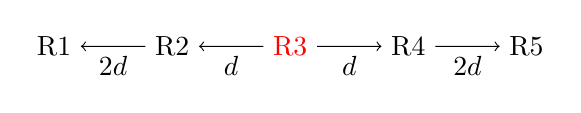
\begin{tikzpicture}[scale = 1.5]
\node (R1) at (.5, .5) {R1};
\node (R2) at (1.5,.5) {R2};
\node (R3) [color =  red]  at (2.5,.5) {R3};
\node (R4) at (3.5,.5) {R4};
\node (R5) at (4.5,.5) {R5};
\draw [->] (R3) -- (R2) node [midway, below] {$d$};
\draw [->] (R3) -- (R4) node [midway, below] {$d$};
\draw [->] (R2) -- (R1) node [midway, below] {$2d$};
\draw [->] (R4) -- (R5) node [midway, below] {$2d$};
\end{tikzpicture}
\end{figure}


When $\mW$ is an inverse distance matrix and its off-diagonal elements are of the form $1/d_{ij}$, where $d_{ij}$ is the distance between two spatial units $i$ and $j$, each row sum is

\begin{equation*}
  1/d + 1/d + 1/2d + 1/2d + .... = 2 \times (1/d + 1/2d + 1/3d + ....) 
\end{equation*}
%
representing a series that is not finite. This is perhaps the main motivation of why some empirical applications introduce a cut-off point $d^*$ such that $w_{ij}=0$ if $d_{ij}>d^*$. However, since the ratio $2 \times (1/d + 1/2d + 1/3d + ....)/ n \to 0$ as $n\to \infty$,  \cite{lee2004asymptotic}'s condition is satisfied, which implies that an inverse distance matrix without cut-off point does not necessarily have to be excluded in an empirical study for reasons of consistency. Thus, Assumption \ref{assu:ml_3} excludes cases where the row sums, $\sum_{j = 1}^n w_{ij}$, for $i = 1,...,n$, diverges to infinity at a rate equal to or faster than the rate of the sample size $n$, because the ML estimator would likely be inconsistent for those cases. Another case where $\left\lbrace h_n \right\rbrace$ is a bounded sequence is when we fixed the number of neighbors, such as in the case of $k$-neighbors approach. Nevertheless our distance example explains why it sometimes leads to numerical problems or unexpected outcomes in empirical applications. This is because the number of unit in the sample generally does not go to infinity, but is finite. 



%Assumptions~\ref{assu:ml_2} is always satisfied if $\left\lbrace h_n \right\rbrace$ is a bounded sequence. Think of $\mW_n$ as spatial weight matrix based on distances that is row-normalized. In this case the $i$th row

%\begin{equation*}
%  w_{i,n} = \frac{(d_{i1}, d_{i2}, ...,d_{in})}{\sum_{j = 1}^nd_{ij}}
%\end{equation*}

%where $d_{ij} > 0$ represents a function of the spatial distance of the $i$th and $j$th units in some space. For a row-normalized $\mW_n$, as $d_{i,j}$ are nonnegative constants and uniformly bounded, if the $\sum_{j = 1}^nd_{ij}, i = 1,...,n$ are uniformly bounded away from zero at the rate $h_n$ in the sense that $\sum_{j = 1}^nd_{ij} =O(h_n)$ uniformly in $i$ and $\lim \inf _{n\to \infty} h_n^{-1}\sum_{j = 1}^nd_{ij} > c$, where $c$ is a positive constant independent of $i$ and $n$, the implied normalized weights matrix will have the property of Assumption \ref{assu:ml_2}.

What if $h_n$ is unbounded? Under this case $\sum_{j = 1}^nd_{ij}$ is uniformly bounded away from zero at the rate $h_n$, where $\lim_{n\to \infty}h_n = \infty$. This particular case \textbf{rules out} cases where each unit has only a (fixed) finite number of neighbors even when the total number of unit increases to infinity. For example, it rules out the case where units correspond to counties and neighbors are defined as counties with contiguous border.

In which cases $h_n \to \infty$? This case requires that each unit in the limit has infinitely many neighbors. As stated by \cite{lee2002consistency}, in economic applications where either the neighbors of any unit are dense in a relevant space or each unit is influenced by many of its neighboring units, which represents a significant proportion of the total population units, it is likely that $\sum_{j = 1}^nd_{ij}$ will diverge and $(1/n)\sum_{j = 1}^nd_{ij}$ will converge as $n$ becomes large. Consider the case where $d_{ij} = 1 / \left|r_i - r_j\right|$, where $r_i$ is the proportion of state $i$'s population that is of African descent. As no state in USA has zero proportion of African-Americans in its population, $d_{ij}$ will be positive, and $(1/n)\sum_{j = 1}^nd_{ij}$ will be bounded away from zero and $\sum_{j = 1}^nd_{ij}$ will be likely to possess the $n$ rate of divergence in this example.

Another example occurs when all cross-sectional units are assumed to be neighbors of each other and are given equal weights. In that case all off-diagonal elements of the spatial weights matrix are $w_{ij} = 1$. Since the row and column sums are $n - 1$, these sums diverge to infinity as $n\to \infty$. In contrast to the previous case, however, $(n - 1)/ n\to 1$ instead of $0$ as $n\to\infty$. This implies that a spatial weight matrix that has equal weights and that is row-normalized subsequently, $w_{ij} - 1 / (n - 1)$ must be excluded for reasons of consistency since is satisfies neither \cite{lee2004asymptotic}'s and  \cite{kelejian1998generalized, kelejian1999generalized}'s condition. The alternative is a group interaction matrix, introduced by Case (1991). Here ``neighbors'' refer to farmers who live in the same district. Suppose that there are $R$ districts and there are $m$ farmers in each district. The sample size is $n = mR$. Case assumed that in a district, each neighbor of a farmer is given equal weight. In that case, $\mW_n  = \mI_R \otimes \mB_m$, where $\mB_m = (\vones_m\vones_m^\top - \mI_m)/(m - 1)$. For this example, $h_n = (m - 1)$ and $h_n/n = (m - 1) / (mR) = O(1/R)$. If sample size $n$ increases by increasing both $R$ and $m$, then $h_n$ goes to infinity and $h_n/n$ goes to zero as $n$ tends to infinity. Thus, this matrix satisfies \cite{lee2004asymptotic}'s condition. 

\begin{remark}
  Whether $\left\lbrace h_n \right\rbrace$ is a bounded or divergent sequence has interesting implications on the OLS estimation. The OLS estimators of $\vbeta$ and $\rho$ are inconsistent when $\left\lbrace h_n \right\rbrace$ is bounded, but they can be consistent when $\left\lbrace h_n \right\rbrace$ is divergent \citep[see][]{lee2002consistency}.
\end{remark}

In summary, when $\left\lbrace h_n \right\rbrace$ is a bounded sequence, it implies a cross sectional unit has only a small number of neighbors, where the spatial dependence is usually defined based on geographical implications. When $\left\lbrace h_n \right\rbrace$ is divergent, it corresponds to the scenario where each unit has a large number of neighbors that often emerges in empirical studies of social interactions or cluster sampling data. 

\begin{assumption}[Non-singularity of $\mA_n$ \citep{lee2004asymptotic}]\label{assu:ml_4}
	The matrix $\mA_n$ is nonsingular.
\end{assumption}

Under Assumption \ref{assu:ml_4}, the SLM (system) has the reduced form (equilibrium) given by
\begin{equation}
\vy = \mA^{-1}_{n0}(\mX_n\vbeta_0 + \vepsi_n)
\end{equation}
%
where $\mA^{-1}_{n0} = (\mI_n - \rho_0\mW_n)$ and with the following expectation and variance:
\begin{eqnarray}
\E(\vy_n)   &=& \left(\mI_n - \rho_0\mW_n\right)^{-1}\mX_n\vbeta  = \mA_{n0}^{-1}\mX_n\vbeta_0\\
\var(\vy_n) &=& \E(\vy_n\vy_n^\top) = \sigma^2_{0}\left(\mI_n - \rho_0\mW_n\right)^{-1}\left[\left(\mI_n - \rho_0\mW_n\right)^{-1}\right]^\top = \sigma^2_0\mA_{n0}^{-1}(\mA_{n0}^{-1})^\top
\end{eqnarray}

We can also write the reduced-form equation as follows:
\begin{equation}
	\begin{aligned}
	\vy_n & = \mX_n\vbeta_0 + \rho_0\mW_n\vy_n + \vepsi_n \\
	      & = \mX_n\vbeta_0 + \rho_0\mW_n\left[\mA^{-1}_n\mX_n\vbeta_0 + \mA^{-1}_n\vepsi_n\right] + \vepsi_n \\
	      & = \mX_n\vbeta_0 + \rho_0\mW_n\mA^{-1}_n\mX_n\vbeta_0 + \rho_0\mW_n\mA^{-1}_n\vepsi_n + \vepsi_n \\
	      & = \mX_n\vbeta_0 + \rho_0\mW_n\mA^{-1}_n\mX_n\vbeta_0  + \left(\mI_n + \rho_0\mW_n\mA^{-1}_n\right)\vepsi_n \\
	      & = \mX_n\vbeta_0 + \rho_0\mC_n\mX_n\vbeta_0  + \left(\mI_n + \rho_0\mC_n\right)\vepsi_n \\
	      & = \mX_n\vbeta_0 + \rho_0\mC_n\mX_n\vbeta_0  +\mA_n^{-1}\vepsi_n
	\end{aligned}
\end{equation}

because $\mI_n + \rho_0\mC_n = \mA_n^{-1}$ (see Exercise  \ref{lab:4.6}), where $\mC_n=\mW_n\mA_n^{-1}$. This expression will also be useful later. 


\begin{assumption}[Uniform boundedness  \citep{lee2004asymptotic}]\label{assu:ml_5}
	The sequences of matrices $\left\lbrace \mW_n \right\rbrace$ and $\left\lbrace \mA_n^{-1} \right\rbrace$ are uniformly bounded in both row and column sums 
\end{assumption}

The uniform boundedness of the matrices is a condition to limit the spatial correlation to a manageable degree. For example, it guarantees that the variances of $\vy_n$ are bounded as $n$ goes to infinity. See our discussion in Section \ref{sec:bounded-matrices}.

Why do we care about this? Because we need the variance goes to zero when the sample size goes to infinity in order to apply some consistency theorem.\footnote{Equivalently, this assumption rules out the unit root case in time series.}

\begin{lemma}[Uniform Boundedness of Matrices in Row and Column Sums]
  Suppose that the spatial weights matrix $\mW_n$ is a non-negative matrix with its $(i,j)$th element being 
  \begin{equation*}
    w_{n,ij} = \frac{d_{ij}}{\sum_{l = 1}^nd_{il}}
  \end{equation*}
  %
  and $d_{ij}>0$ for all $i,j$.
  
  \begin{enumerate}
    \item If the row sums $\sum_{j = 1}^nd_{ij}$ are bounded away from zero at the rate $h_n$ uniformly in $i$, and the column sums $\sum_{i = 1}^nd_{ij}$ are $O(h_n)$ uniformly in $j$, then $\left\lbrace \mW_n \right\rbrace$  are uniformly bounded in column sums.
    \item (Symmetric Matrix) If $d_{ij} = d_{ji}$ for all $i$ and $j$ and the row sums $\sum_{j = 1}^nd_{ij}$ are $O(h_n)$ and bounded away from zero at the rate $h_n$ uniformly in $i$, then $\left\lbrace \mW_n \right\rbrace$  are uniformly bounded in column sums.
  \end{enumerate}
\end{lemma}

\begin{assumption}[No asymptotic multicollinearity \citep{lee2004asymptotic}]\label{assu:ml_6}
	The elements of $\mX_n$ are uniformly bounded constants for all $n$. The $\lim_{n\to \infty}\mX_n^\top\mX_n/n$ exists and is nonsingular. 
\end{assumption}

This rules out multicollinearity among the regressors. Note also that we are assuming that $\mX_n$ is \textbf{nonstochastic}. If $\mX_n$ were stochastic, then we will require:
\begin{equation*}
  \plim_{n\to \infty}\mX_n^\top\mX_n/ n,
\end{equation*}

to exists.

\begin{assumption}[Uniform Boundedness of ${\mA_n^{-1}(\rho)}$ \cite{lee2004asymptotic}]\label{assu:ml_7}
	${\mA_n^{-1}(\rho)}$ are uniformly bounded in either row or column sums, uniformly in $\rho$ in a compact parameter space $\Gamma$. The true parameter $\rho_0$ is in the interior of $\Gamma$
\end{assumption}

This assumption is needed to deal with the nonlinearity of $\log \left|\left(\mI_n - \rho \mW\right)^{-1}\right|$ in the log-likelihood function. Recall that if $\left\| \mW\right\| < 1$, then $\mI_n - \rho\mW_n$ is invertible for all $n$. Then if $\left\| \mW\right\| < 1$, then the sequence of matrices $\left\|\left(\mI_n- \mW_n\right)^{-1}\right\|$ are uniformly bounded in any subset of $(-1, 1)$ bounded away from the boundary. As we previously see, if $\mW_n$ is row-standardized $\left(\mI_n- \mW\right)^{-1}$ is uniformly bounded in row sums norm uniformly in any closed subset of $(-1, 1)$. Therefore, $\Gamma$ from Assumption~\ref{assu:ml_7} can be considered as a single closed set contained in (-1, 1).

What if $\mW_n$ is not row-normalized but its eigenvalues are real? Then, the Jacobian of $\left|\left(\mI_n- \mW\right)^{-1}\right|$ will be positive if $-1/\omega_{min} < \rho < 1/\omega_{max}$, where $\omega_{min}$ and $\omega_{max}$ are the minimum and maximum eigenvalues of $\mW_n$, and $\Gamma$ will be a closed interval contained in $(-1/\omega_{min}, 1/\omega_{max})$ for all $n$. Thus, Assumption~\ref{assu:ml_7} rules out models where $\rho_0$ is close to -1 and 1.  

\begin{assumption}[Identification \citep{lee2004asymptotic}]\label{assu:ml_8}
		The
		\begin{equation*}
			\lim_{n\to \infty}\frac{1}{n}\left(\mX_n, \mC_n\mX_n\vbeta_0\right)'\left(\mX_n, \mC_n\mX_n\vbeta_0\right)
		\end{equation*}
		%
		 exists and is nonsingular.
\end{assumption}

This is a sufficient condition for global identification of $\vtheta_0$

\begin{theorem}[Consistency]\label{teorem:Consistency_ML}
	Under assumption \ref{assu:ml_1}-\ref{assu:ml_8}, $\vtheta_0$ is globally identifiable and $\widehat{\vtheta}_n$ is a consistent estimator of $\vtheta_0$.
\end{theorem}

Identification of $\rho_0$ can be based on the maximum values of the concentrated log-likelihood function $Q_n(\rho) / n$. With identification and uniform convergence of $\left[\log L_n(\rho) - Q_n(\rho)\right] / n$ to zero on $\Gamma$, consistency of the QMLE $\widehat{\vtheta}_n$ follows. The sketch of the proof for Theorem \ref{teorem:Consistency_ML} is given in Appendix \ref{appendix-consistency}. 

For a proof without compactness of the parameter space (proving concavity of the log-likelihood function) see \cite{liu2022consistency}.

%=====================================
\subsection{Asymptotic Normality}
%=====================================

To derive the asymptotic distribution of the QML and ML we need the asymptotic behavior of the gradient. Taking a Taylor series expansion around $\vtheta_0$ of $\partial \ell_n(\widehat{\vtheta}_n)/ \partial \vtheta = 0$ at $\vtheta_0$, we get
\begin{equation}
  \frac{\partial \ell_n(\widehat{\vtheta}_n)}{\partial \vtheta} =  \frac{\partial \ell_n(\vtheta_0)}{\partial \vtheta} + \frac{\partial^2 \ell_n(\widetilde{\vtheta}_n)}{\partial \vtheta \partial \vtheta^\top}(\widehat{\vtheta}_n - \vtheta_0),
\end{equation}
%
where $\widetilde{\vtheta}_n = \alpha_n \widehat{\vtheta}_n + (1 - \alpha_n)\vtheta_0$ and $\alpha_n\in \left[ 0, 1\right]$, therefore:
\begin{equation}\label{eq:sampling-error-ml}
  \sqrt{n}(\widehat{\vtheta}_n - \vtheta_0) = - \left[\frac{1}{n}\frac{\partial^2 \ell_n(\widetilde{\vtheta}_n)}{\partial \vtheta \partial \vtheta^\top}\right]^{-1}\frac{1}{\sqrt{n}}\frac{\partial \ell_n(\vtheta_0)}{\partial \vtheta}.
\end{equation}

As standard in asymptotic theory of MLE, we need to show that the first element of the rhs of \eqref{eq:sampling-error-ml} converges to something. We also need to find the limiting distribution of $\frac{1}{\sqrt{n}}\frac{\partial \ell_n(\vtheta_0)}{\partial \vtheta}$. Recall that the first-order derivatives of the log-likelihood function \textbf{evaluated at $\vtheta_0$} are given by (see Section \ref{sec:score_sml}):

\begin{align}
	\frac{1}{\sqrt{n}}\frac{\partial \ell_n(\vtheta_0)}{\partial \vbeta} & = \frac{1}{\sigma^2_0\sqrt{n}}\mX_n^\top\vepsi_n \\
	\frac{1}{\sqrt{n}}\frac{\partial \ell_n(\vtheta_0)}{\partial \sigma^2} & = \frac{1}{2\sigma_0^4\sqrt{n}}\left(\vepsi_n'\vepsi_n - n\sigma_0^2\right) \\
		\frac{1}{\sqrt{n}}\frac{\partial \ell_n(\vtheta_0)}{\partial \rho} & = \frac{1}{\sigma_0^2\sqrt{n}}(\mC_{n0}\mX_n\vbeta_0)^\top \vepsi_n + \frac{1}{\sigma_0^2\sqrt{n}}(\vepsi_n^\top\mC_{n0}\vepsi_n - \sigma_0^2\tr(\mC_{n0}))\label{eq:asy_der_rho}
\end{align}	

As explained by \citet[][pag. 1905]{lee2004asymptotic}, these are linear and quadratic functions of $\vepsi_n$. In particular, the asymptotic distribution of (\ref{eq:asy_der_rho}) may be derived from central limit theorem for linear-quadratic forms. The matrix $\mC_{n0}$ is uniformly bounded in row sums. As the elements of $\mX_n$ are bounded, the elements of $\mC_{n0}\mX_n\vbeta_0$ for all $n$ are uniformly bounded by Lemma \ref{lemma:bounded_lemma}. With the existence of high order moments of $\epsilon$ in Assumption \ref{assu:ml_1}, the central limit theorem for quadratic forms of double arrays of \cite{kelejian2001asymptotic} can be applied and the limit distribution of the score vector follows.

Since $\E\left[(1 / \sqrt{n}) \partial \ell_n /\partial \vtheta\right]  = \vzeros$,  the variance matrix of $(1 / \sqrt{n}) \partial \ell_n /\partial \vtheta$ is:
\begin{equation}
  \E\left[\frac{1}{\sqrt{n}}\frac{\partial \ell_n (\vtheta_0)}{\partial \vtheta}\cdot\frac{1}{\sqrt{n}}\frac{\partial \ell_n (\vtheta_0)}{\partial \vtheta^\top} \right] = - \E\left(\frac{1}{n} \frac{\partial \ell_n(\vtheta)}{\partial \vtheta \partial \vtheta^\top}\right) + \mOmega_{\vtheta, n},
\end{equation}
%
where 
\begin{equation}\label{eq:expected-hessian-slm-asy}
- \E\left(\frac{1}{n} \frac{\partial \log L_n(\vtheta)}{\partial \vtheta \partial \vtheta^\top}\right)= 
	\begin{pmatrix}
	\frac{1}{\sigma^2n}(\mX_n^\top \mX_n) & \vzeros^\top & \frac{1}{\sigma^2n} \mX_n^\top (\mC_n\mX_n\vbeta) \\
		 &  \frac{1}{2\sigma^4} & \frac{1}{\sigma^2n} \tr(\mC_n)\\
		 &  & \frac{1}{n}\tr(\mC^s_n\mC_n) + \frac{1}{\sigma^2n}(\mC_n\mX_n\vbeta)^\top(\mC_n\mX_n\vbeta)
	\end{pmatrix} 
\end{equation}
%
and $\mC^s_n = \mC_n + \mC_n^\top$. Equation \ref{eq:expected-hessian-slm-asy} represents the average Hessian matrix (or information matrix when $\vepsi$'s are \textbf{normal}). The matrix $ \mOmega_{\vtheta, n}$ is a matrix with the second, third, and fourth moments of $\vepsi$. If $\vepsi_n$ is normally distributed, then $\mOmega_{\vtheta, n} = \vzeros$. Derivation of \ref{eq:expected-hessian-slm-asy} is given in Appendix \ref{appendix-EH-sml}.

\begin{theorem}[Asymptotic Normality]
Under Assumptions \ref{assu:ml_1}-\ref{assu:ml_8}, 

\begin{equation}
  \sqrt{n}\left(\widehat{\vtheta}_n- \vtheta_0\right)\dto \rN\left(\vtheta, \mSigma_{\vtheta}^{-1} + \mSigma_{\vtheta}^{-1}\mOmega_{\vtheta}\mSigma_{\vtheta}^{-1}\right),
\end{equation}
%
where $\mOmega_{\vtheta} = \lim_{n\to\infty}\mOmega_{\vtheta, n}$ and

\begin{equation}
  \mSigma_{\vtheta}= - \lim_{n\to\infty} \E\left[\frac{1}{n}\frac{\partial^2 \log L_n(\vtheta_0)}{\partial \vtheta \partial \vtheta^\top}\right],
\end{equation}
which are assumed to exists. If the $\epsilon_i$'s are \textbf{normally distributed}, then:

\begin{equation}
  \sqrt{n}\left(\widehat{\vtheta}_n- \vtheta_0\right)\dto \rN\left(\vtheta, \mSigma_{\vtheta}^{-1}\right).
\end{equation}
\end{theorem}

%=====================================
\section{Computing the Standard Errors For The Marginal Effects}
%=====================================

In section \ref{sec:summary-measures}, we explain how to obtain summary measures for the direct, indirect and total effects. However, we did not explain how to obtain standard errors for such measures. For example, we would like to have confidence intervals for the indirect effects and to be able to say whether they are significant. 

Recall that our three summary measures are:

\begin{eqnarray*}
\bar{M}(\vtheta)_{\mbox{direct}} & = & n^{-1}\tr\left(\mS_r(\vtheta)\right) \\
\bar{M}(\vtheta)_{\mbox{total}} & = & n^{-1}\vones_n^\top\mS_r(\vtheta)\vones_n \\
\bar{M}(\vtheta)_{\mbox{indirect}} & = & \bar{M}(r)_{\mbox{total}} - \bar{M}(r)_{\mbox{direct}},
\end{eqnarray*}
%
which are highly nonlinear due to $\mS_r(\vtheta)$.\footnote{Note that we have replaced the parameter for the spatially lagged independent variable to let $\vtheta$ be the vector parameters of the model. } Therefore, a procedure such as the Delta Method is not feasible. Instead, we use a Monte Carlo approximation which takes into account the sampling distribution of $\vtheta$. To show this procedure, consider the SDM where:

\begin{equation*}
\mS(\vtheta)_r = \left(\mI_n - \rho\mW\right)^{-1}\left(\mI_n\beta_r + \mW\gamma_r\right)
\end{equation*}


Let $g(\vtheta)= \bar{M}(\vtheta)$ be a function representing the marginal (direct, indirect or total) effect that depends on the population parameters $\vtheta$. If $\rN(\vtheta|\bar{\vtheta}, \mSigma_{\theta})$ denotes the multivariate normal density of $\vtheta$ with mean $\bar{\vtheta}$ and asymptotic variance-covariance matrix $\mSigma_{\theta}$, then the expected value of the marginal effects conditional on the population parameters $\bar{\vtheta}$ and $\mSigma_{\theta}$ is:

\begin{equation}
\E(g(\vtheta)|\bar{\vtheta}, \mSigma_{\theta}) = \int_{\vtheta}\E(g(\vtheta)|\vy, \mX, \vtheta)\rN(\vtheta|\bar{\vtheta}, \mSigma_{\theta})d\vtheta. 
\end{equation}

A Monte Carlo approximation to this expectation is obtained by calculation of the empirical marginal effects evaluated at pseudo draws of $\vtheta$ from the asymptotic distribution of the estimator. The algorithm is the following:

\begin{algorithm}[Standard Errors of the Marginal Effects]
Estimate the model using MLE. Consider $s = 1, ..., S$, and start with $s = 1$
\begin{enumerate}
  \item Take a random draw of $\vtheta^{s}$ from $\rN(\widehat{\bar{\vtheta}}, \widehat{\mSigma}_{\theta})$, which is the estimated asymptotic distribution of $\widehat{\vtheta}$. 
 \item Compute the marginal effect, but substituting  $\widehat{\vtheta}$ for $\vtheta^s$. 
 \item Update $s = s + 1$, and go back to step 1. 
 \item Repeat for a large number of repetitions S (e.g., S = 1000).  
 \item Calculate the empirical mean of the marginal effects. The standard error of the marginal effect across the $S$ draws is the standard error. 
\end{enumerate}
\end{algorithm}


%====================================
\section{Spillover Effects on Crime: An Application in R}\label{sec:Anselin-example}
%====================================


\subsection{Estimation of Spatial Models in R}

In this example we use \cite{anselin1988spatial}'s dataset. This sample corresponds to a cross-sectional dataset of 49 Columbus, Ohio neighborhoods, which is used to explain the crime rate as  a function of household income and housing values. In particular, the variables  are the following:

\begin{itemize}
  \item \texttt{CRIME}: residential burglaries and vehicle thefts per thousand household in the neighborhood.
  \item \texttt{HOVAL}: housing value in US\$1,000.
  \item \texttt{INC}: household income in US\$1,000.
\end{itemize}

We start our analysis by loading the required packages into \proglang{R} workspace.

\begin{knitrout}
\definecolor{shadecolor}{rgb}{0.969, 0.969, 0.969}\color{fgcolor}\begin{kframe}
\begin{alltt}
\hlcom{# Load packages}
\hlkwd{library}\hlstd{(}\hlstr{"spdep"}\hlstd{)}
\hlkwd{library}\hlstd{(}\hlstr{"spatialreg"}\hlstd{)}
\hlkwd{library}\hlstd{(}\hlstr{"memisc"}\hlstd{)}            \hlcom{# Package for tables}
\hlkwd{library}\hlstd{(}\hlstr{"maptools"}\hlstd{)}
\hlkwd{library}\hlstd{(}\hlstr{"RColorBrewer"}\hlstd{)}
\hlkwd{library}\hlstd{(}\hlstr{"classInt"}\hlstd{)}
\hlkwd{source}\hlstd{(}\hlstr{"getSummary.sarlm.R"}\hlstd{)} \hlcom{# Function for spdep models}
\end{alltt}
\end{kframe}
\end{knitrout}

The dataset is currently part of the \pkg{spdep} package. We load the data using the following commands.

\begin{knitrout}
\definecolor{shadecolor}{rgb}{0.969, 0.969, 0.969}\color{fgcolor}\begin{kframe}
\begin{alltt}
\hlcom{# Load data}
\hlstd{columbus}   \hlkwb{<-} \hlkwd{readShapePoly}\hlstd{(}\hlkwd{system.file}\hlstd{(}\hlstr{"etc/shapes/columbus.shp"}\hlstd{,}
                                      \hlkwc{package} \hlstd{=} \hlstr{"spdep"}\hlstd{)[}\hlnum{1}\hlstd{])}
\hlstd{col.gal.nb} \hlkwb{<-} \hlkwd{read.gal}\hlstd{(}\hlkwd{system.file}\hlstd{(}\hlstr{"etc/weights/columbus.gal"}\hlstd{,}
                                   \hlkwc{package} \hlstd{=} \hlstr{"spdep"}\hlstd{)[}\hlnum{1}\hlstd{])}
\end{alltt}
\end{kframe}
\end{knitrout}

As usual in applied work, we start the analysis by asking whether there exists a spatial pattern in the variable we are interested in. To get some insights about the spatial distribution of \code{CRIME} we use the following quantile clorophet graph:

\begin{knitrout}
\definecolor{shadecolor}{rgb}{0.969, 0.969, 0.969}\color{fgcolor}\begin{kframe}
\begin{alltt}
\hlcom{# Spatial distribution of crime}
\hlkwd{spplot}\hlstd{(columbus,} \hlstr{"CRIME"}\hlstd{,}
       \hlkwc{at} \hlstd{=} \hlkwd{quantile}\hlstd{(columbus}\hlopt{$}\hlstd{CRIME,} \hlkwc{p} \hlstd{=} \hlkwd{c}\hlstd{(}\hlnum{0}\hlstd{,} \hlnum{.25}\hlstd{,} \hlnum{.5}\hlstd{,} \hlnum{.75}\hlstd{,} \hlnum{1}\hlstd{),} \hlkwc{na.rm} \hlstd{=} \hlnum{TRUE}\hlstd{),}
       \hlkwc{col.regions} \hlstd{=} \hlkwd{brewer.pal}\hlstd{(}\hlnum{5}\hlstd{,} \hlstr{"Blues"}\hlstd{),}
       \hlkwc{main} \hlstd{=} \hlstr{""}\hlstd{)}
\end{alltt}
\end{kframe}
\end{knitrout}

Figure \ref{fig:spatial-crime} shows the spatial pattern of crime. It can be observed that the spatial distribution of crime follows a clear pattern of positive autocorrelation. However, we must corroborate this statement by using a global test of spatial autocorrelation. To do so, we use a row-normalized binary contiguity matrix $\mW$, \code{col.gal.nb},  based on the queen criteria and carry out a Moran's I test. In particular, we use a Moran test based on Monte Carlo simulations using the \code{moran.mc} function with 99 simulations. 

\begin{figure}[ht]
\caption{Spatial Distribution of Crime in Columbus, Ohio Neighborhoods}
    \label{fig:spatial-crime}
    \centering 
	\begin{minipage}{.9\linewidth}
\begin{knitrout}
\definecolor{shadecolor}{rgb}{0.969, 0.969, 0.969}\color{fgcolor}

{\centering \includegraphics[width=9cm,height=9cm]{figure/spatial-crime-1} 

}


\end{knitrout}
\footnotesize
		\emph{Notes:} This graph shows the spatial distribution of crime on the 49 Columbus, Ohio neighborhoods. Darker color indicates greater rate of crime. 
	\end{minipage}	
\end{figure}


\begin{knitrout}
\definecolor{shadecolor}{rgb}{0.969, 0.969, 0.969}\color{fgcolor}\begin{kframe}
\begin{alltt}
\hlcom{# Moran's I test}
\hlkwd{set.seed}\hlstd{(}\hlnum{1234}\hlstd{)}
\hlstd{listw} \hlkwb{<-} \hlkwd{nb2listw}\hlstd{(col.gal.nb,} \hlkwc{style} \hlstd{=} \hlstr{"W"}\hlstd{)}
\hlkwd{moran.mc}\hlstd{(columbus}\hlopt{$}\hlstd{CRIME,} \hlkwc{listw} \hlstd{= listw,}
           \hlkwc{nsim} \hlstd{=} \hlnum{99}\hlstd{,} \hlkwc{alternative} \hlstd{=} \hlstr{'greater'}\hlstd{)}
\end{alltt}
\begin{verbatim}
## 
## 	Monte-Carlo simulation of Moran I
## 
## data:  columbus$CRIME 
## weights: listw  
## number of simulations + 1: 100 
## 
## statistic = 0.48577, observed rank = 100, p-value = 0.01
## alternative hypothesis: greater
\end{verbatim}
\end{kframe}
\end{knitrout}

The results show that the Moran's I statistic is 0.51 and the p-value is 0.01. This implies that we reject the null hypothesis of random spatial distribution and there exists evidence of positive global spatial autocorrelation in the crime variable: places with high (low) crime rate are surrounded by places with high (low) crime rate. 

Our next step is to estimate different spatial models using the functions already programmed in \pkg{spatialreg}. First, we estimate the classical OLS model followed by the SLX, SLM, SDM, SEM and SAC models. The functions used for each models are the following:

\begin{itemize}
  \item OLS: \code{lm} function.
  \item SLX: \code{lm} function, where $\mW\mX$ is constructed using the function \code{lag.listw} from \pkg{spdep} package. This model can also be estimated using the function \code{lmSLX} from \pkg{spatialreg} package as shown below. 
  \item SLM: \code{lagsarlm} from \pkg{spatialreg} package.  
  \item SDM: \code{lagsarlm} from \pkg{spatialreg} package, using the argument \code{type = "mixed"}. Note that \code{type = "Durbin"} may be used instead of \code{type = "mixed"}. 
  \item SEM: \code{errorsarlm} from \pkg{spatialreg} package. Note that the Spatial Durbin Error Model (SDEM)---not shown here--- can be estimated by using  \code{type = "emixed"}. 
  \item SAC: \code{sacsarlm} from \pkg{spatialreg} package.
\end{itemize}

All models are estimated using ML procedure outline in the previous section. In order to compute the determinant of the Jacobian we use the \cite{ord1975estimation}'s procedure by explicitly using the argument \code{method = "eigen"} in each spatial model. That is, the Jacobian is computed as in (\ref{eq:Ord-determinant}).

\begin{knitrout}
\definecolor{shadecolor}{rgb}{0.969, 0.969, 0.969}\color{fgcolor}\begin{kframe}
\begin{alltt}
\hlcom{# Models}
\hlstd{columbus}\hlopt{$}\hlstd{lag.INC}   \hlkwb{<-} \hlkwd{lag.listw}\hlstd{(listw,}
                         \hlstd{columbus}\hlopt{$}\hlstd{INC)}   \hlcom{# Create spatial lag of INC}
\hlstd{columbus}\hlopt{$}\hlstd{lag.HOVAL} \hlkwb{<-} \hlkwd{lag.listw}\hlstd{(listw,}
                         \hlstd{columbus}\hlopt{$}\hlstd{HOVAL)} \hlcom{# Create spatial lag of HOVAL}
\hlstd{ols} \hlkwb{<-} \hlkwd{lm}\hlstd{(CRIME} \hlopt{~} \hlstd{INC} \hlopt{+} \hlstd{HOVAL,}
          \hlkwc{data} \hlstd{=  columbus)}
\hlstd{slx} \hlkwb{<-} \hlkwd{lm}\hlstd{(CRIME} \hlopt{~} \hlstd{INC} \hlopt{+} \hlstd{HOVAL} \hlopt{+} \hlstd{lag.INC} \hlopt{+} \hlstd{lag.HOVAL,}
          \hlkwc{data} \hlstd{=  columbus)}
\hlstd{slm} \hlkwb{<-} \hlkwd{lagsarlm}\hlstd{(CRIME} \hlopt{~} \hlstd{INC} \hlopt{+} \hlstd{HOVAL,}
                \hlkwc{data} \hlstd{= columbus,}
                \hlstd{listw,}
                \hlkwc{method} \hlstd{=} \hlstr{"eigen"}\hlstd{)}
\hlstd{sdm} \hlkwb{<-} \hlkwd{lagsarlm}\hlstd{(CRIME} \hlopt{~} \hlstd{INC} \hlopt{+} \hlstd{HOVAL,}
                \hlkwc{data} \hlstd{= columbus,}
                \hlstd{listw,}
                \hlkwc{method} \hlstd{=} \hlstr{"eigen"}\hlstd{,}
                \hlkwc{type} \hlstd{=} \hlstr{"mixed"}\hlstd{)}
\hlstd{sem} \hlkwb{<-} \hlkwd{errorsarlm}\hlstd{(CRIME} \hlopt{~} \hlstd{INC} \hlopt{+} \hlstd{HOVAL,}
                \hlkwc{data} \hlstd{= columbus,}
                \hlstd{listw,}
                \hlkwc{method} \hlstd{=} \hlstr{"eigen"}\hlstd{)}
\hlstd{sac} \hlkwb{<-} \hlkwd{sacsarlm}\hlstd{(CRIME} \hlopt{~} \hlstd{INC} \hlopt{+} \hlstd{HOVAL,}
                \hlkwc{data} \hlstd{= columbus,}
                \hlstd{listw,}
                \hlkwc{method} \hlstd{=} \hlstr{"eigen"}\hlstd{)}
\end{alltt}
\end{kframe}
\end{knitrout}

Note that the SLX model can also be estimated as follows:

\begin{knitrout}
\definecolor{shadecolor}{rgb}{0.969, 0.969, 0.969}\color{fgcolor}\begin{kframe}
\begin{alltt}
\hlstd{slx2} \hlkwb{<-} \hlkwd{lmSLX}\hlstd{(CRIME} \hlopt{~} \hlstd{INC} \hlopt{+} \hlstd{HOVAL,}
              \hlkwc{data} \hlstd{= columbus,}
              \hlstd{listw)}
\hlkwd{summary}\hlstd{(slx2)}
\end{alltt}
\end{kframe}
\end{knitrout}



The models are presented in Table \ref{tab:columbus-models}. The OLS estimates are presented in the first column. The results show that an increase of one  thousand dollars in the income of the neighborhood is correlated, in average, with a decreased of 1.6 crimes per thousand households. Similarly, an increase of one thousand dollars in the housing value of the neighborhood is correlated, on average, with a decreased of 0.3 crimes per thousand households. Both correlations are statistically significant.\footnote{Note that we refer to correlation since there may still be some sort of endogeneity problem in either of the two variables.} Both results implies that crimes (residential burglaries and vehicle thefts) are lower in richer neighborhoods. 

Column 2 of Table \ref{tab:columbus-models} show the results for the SLX. In particular, the model is given by $\vy = \mX\vbeta + \mW\mX\vgamma + \vepsi$, where $\mW\mX$ is a $49\times 2$ matrix, whose columns correspond to the spatial lag of \code{INC} and \code{HOVAL}. The coefficient for the spatial lag of \code{INC}, \code{W.INC}, is negative and significant. This implies that crime in spatial unit $i$ is correlated with the income in its neighborhood: the higher the income of the neighbors of $i$ the lower the crime in $i$. This result does not, however, hold for the housing value of the neighbors of $i$ which is positive but not statistically different from zero. 

The results for the SLM are shown in column 3. The spatial autoregressive parameter $\rho$ is positive and significant indicating strong spatial autocorrelation. This implies evidence of spillover effects on crime. The coefficients for the other variables in the regression are similar to the OLS results, though smaller in absolute value.

The results for the SDM are presented in column 4. Whereas the estimated $\rho$ parameter is positive and significant, the coefficient of the lagged explanatory variables are not. This indicates that once we have take into account the endogenous interaction effects of crime, the neighbors' factors do not matter in explaining the crime in each location. Moreover, for the spatial lag of income, the wrong sign is obtained, since the common factor hypothesis would imply a positive sign, given a positive estimate for $\rho$ and negative sign for INC. This provide some evidence that an omitted spatial lag may be the main spatial effect, rather than spatial dependence in the error term. 

Column 5 shows the results for the the SEM model which confirm the conclusions from the previous models. It can be noticed that the autoregressive parameter for $\mW\vu$ is positive and significant indicating an important spatial transmission of the random shocks. This result may be explained by the fact of omitting important variables that are spatially correlated. 

The SAC model, presented in column 6, considers both endogenous interactions effects and interactions effects among the error terms. From the results, we observe that the SAC model produces coefficients estimates of $\mW\vy$ and $\mW\vu$ variables that are not significantly different from zero. However, if endogenous interaction effects and interactions effects among the error terms are separated from each other, both coefficients turn out to be significant. This might be explained by the fact that the model is overparametrized, as a result of which the significance levels of all variables tend to go down. 


\begin{table}[ht]
\caption{Spatial Models for Crime in Columbus, Ohio Neighborhoods.}\label{tab:columbus-models}
\centering
\begin{tabular}{lD{.}{.}{3}D{.}{.}{3}D{.}{.}{3}D{.}{.}{3}D{.}{.}{3}D{.}{.}{3}}
\toprule
 & 
\multicolumn{1}{c}{OLS} & 
\multicolumn{1}{c}{SLX} & 
\multicolumn{1}{c}{SLM} & 
\multicolumn{1}{c}{SDM} & 
\multicolumn{1}{c}{SEM} & 
\multicolumn{1}{c}{SAC}\\
\midrule
\emph{Constant} & 68.619^{***} & 74.029^{***} & 46.851^{***} & 45.593^{***} & 61.054^{***} & 49.051^{***}\\
                 & (4.735) & (6.722) & (7.315) & (13.129) & (5.315) & (10.055)\\
INC              & -1.597^{***} & -1.108^{**} & -1.074^{***} & -0.939^{**} & -0.995^{**} & -1.069^{**}\\
                 & (0.334) & (0.375) & (0.311) & (0.338) & (0.337) & (0.333)\\
HOVAL            & -0.274^{*} & -0.295^{**} & -0.270^{**} & -0.300^{***} & -0.308^{***} & -0.283^{**}\\
                 & (0.103) & (0.101) & (0.090) & (0.091) & (0.093) & (0.092)\\
$W.INC$          &  & -1.383^{*} &  & -0.618 &  & \\
                 &  & (0.559) &  & (0.577) &  & \\
$W.HOVAL$        &  & 0.226 &  & 0.267 &  & \\
                 &  & (0.203) &  & (0.184) &  & \\
$\rho$          &  &  & 0.404^{***} & 0.383^{*} &  & 0.353\\
                 &  &  & (0.121) & (0.162) &  & (0.197)\\
$\lambda$       &  &  &  &  & 0.521^{***} & 0.132\\
                 &  &  &  &  & (0.141) & (0.299)\\
\midrule
AIC              & 382.754 & 380.197 & 376.337 & 378.032 & 378.310 & 378.146\\
N                &  49     &  49     &  49     &  49     &  49     &  49    \\
\bottomrule
\multicolumn{7}{p{.7\linewidth}}{Significance: 
              $*** \equiv p < 0{.}001$; 
              $** \equiv p < 0{.}01$; 
              $* \equiv p < 0{.}05$}\\
\end{tabular}

\end{table}

%---------------------------------------------------
\subsection{Estimation of Marginal Effects in R}
%---------------------------------------------------

In this Section we expand our analysis from Section \ref{sec:lesage-example} in the sense that we now integrate the estimation of the marginal effects using a real estimation from \proglang{R}. 

We begin our analysis with the following question: what would happen to crime in all regions if income rose from 13.906 to 14.906 in the 30th region ($\Delta\texttt{INC} = 1$)? Note that we tried to answer a similar question in the commuting-time example from previous chapter. As we did in Section \ref{sec:lesage-example} we can use the reduced-form predictor given by the following formula:

\begin{equation*}
\widehat{\vy} = \E(\vy| \mX, \mW) = (\mI_n - \widehat{\rho}\mW)^{-1}\mX\widehat{\vbeta},
\end{equation*}
% 
and estimate the predicted values pre- and post- the change in the income variable. In the following lines we use the reduced-form predictor and the observed values of the exogenous variables to obtain the predicted values for \code{CRIME}, $\widehat{\vy}^1$,  using the SLM model previously estimated. 
  
\begin{knitrout}
\definecolor{shadecolor}{rgb}{0.969, 0.969, 0.969}\color{fgcolor}\begin{kframe}
\begin{alltt}
\hlcom{# The predicted values}
\hlstd{rho}       \hlkwb{<-} \hlstd{slm}\hlopt{$}\hlstd{rho}                                \hlcom{# Estimated rho from SLM model}
\hlstd{beta_hat}  \hlkwb{<-} \hlkwd{coef}\hlstd{(slm)[}\hlopt{-}\hlnum{1}\hlstd{]}                          \hlcom{# Estimated parameters}
\hlstd{A}         \hlkwb{<-} \hlkwd{invIrW}\hlstd{(listw,} \hlkwc{rho} \hlstd{= rho)}               \hlcom{# (I - rho*W)^\{-1\}}
\hlstd{X}         \hlkwb{<-} \hlkwd{cbind}\hlstd{(}\hlnum{1}\hlstd{, columbus}\hlopt{$}\hlstd{INC, columbus}\hlopt{$}\hlstd{HOVAL)} \hlcom{# Matrix of observed variables}
\hlstd{y_hat_pre} \hlkwb{<-} \hlstd{A} \hlopt \hlkwd{crossprod}\hlstd{(}\hlkwd{t}\hlstd{(X), beta_hat)}        \hlcom{# y hat}
\end{alltt}
\end{kframe}
\end{knitrout}

Next we increase \code{INC} by 1 in spatial unit 30, and calculate the reduced-form predictions, $\widehat{\vy}^2$.

\begin{knitrout}
\definecolor{shadecolor}{rgb}{0.969, 0.969, 0.969}\color{fgcolor}\begin{kframe}
\begin{alltt}
\hlcom{# The post-predicted values}
\hlstd{col_new} \hlkwb{<-} \hlstd{columbus} \hlcom{# copy the data frame}

\hlcom{# Change the income value}
\hlstd{col_new}\hlopt{@}\hlkwc{data}\hlstd{[col_new}\hlopt{@}\hlkwc{data}\hlopt{$}\hlstd{POLYID} \hlopt{==} \hlnum{30}\hlstd{,} \hlstr{"INC"}\hlstd{]} \hlkwb{<-} \hlnum{14.906}

\hlcom{# The predicted values}
\hlstd{X_d}        \hlkwb{<-} \hlkwd{cbind}\hlstd{(}\hlnum{1}\hlstd{, col_new}\hlopt{$}\hlstd{INC, col_new}\hlopt{$}\hlstd{HOVAL)}
\hlstd{y_hat_post} \hlkwb{<-} \hlstd{A} \hlopt \hlkwd{crossprod}\hlstd{(}\hlkwd{t}\hlstd{(X_d), beta_hat)}
\end{alltt}
\end{kframe}
\end{knitrout}

Finally,  we compute the difference between pre- and post-predictions: $\widehat{\vy}^2 - \widehat{\vy}^1$:

\begin{knitrout}
\definecolor{shadecolor}{rgb}{0.969, 0.969, 0.969}\color{fgcolor}\begin{kframe}
\begin{alltt}
\hlcom{# The difference}
\hlstd{delta_y}         \hlkwb{<-} \hlstd{y_hat_post} \hlopt{-} \hlstd{y_hat_pre}
\hlstd{col_new}\hlopt{$}\hlstd{delta_y} \hlkwb{<-} \hlstd{delta_y}

\hlcom{# Show the effects}
\hlkwd{summary}\hlstd{(delta_y)}
\end{alltt}
\begin{verbatim}
##        V1            
##  Min.   :-1.1141241  
##  1st Qu.:-0.0074114  
##  Median :-0.0012172  
##  Mean   :-0.0336341  
##  3rd Qu.:-0.0002604  
##  Max.   :-0.0000081
\end{verbatim}
\begin{alltt}
\hlkwd{sum}\hlstd{(delta_y)}
\end{alltt}
\begin{verbatim}
## [1] -1.648071
\end{verbatim}
\end{kframe}
\end{knitrout}

According to the result from \code{sum(delta\_y)},  the predicted effect of the change would be a decrease of 1.65 in the crime rate, considering both direct and indirect effects. That is, increasing the income in US\$1,000 in region 30th might generate effects that will transmit through the whole system of region resulting in a new equilibrium where the the total crime will reduce in 1.7 crimes per thousand households. 

Sometimes we would like to plot these effects. Suppose we wanted to show those regions that had low and high impact due to the increase in \code{INC}. Let's define ``high impacted regions'' those regions whose crime rate decrease more than 0.05. The following code produces Figure \ref{fig:predicted-effect}. 

\begin{knitrout}
\definecolor{shadecolor}{rgb}{0.969, 0.969, 0.969}\color{fgcolor}\begin{kframe}
\begin{alltt}
\hlcom{# Breaks}
\hlstd{breaks} \hlkwb{<-} \hlkwd{c}\hlstd{(}\hlkwd{min}\hlstd{(col_new}\hlopt{$}\hlstd{delta_y),} \hlopt{-}\hlnum{0.05}\hlstd{,} \hlkwd{max}\hlstd{(col_new}\hlopt{$}\hlstd{delta_y))}
\hlstd{labels} \hlkwb{<-} \hlkwd{c}\hlstd{(}\hlstr{"High-Impacted Regions"}\hlstd{,} \hlstr{"Low-Impacted Regions"}\hlstd{)}
\hlstd{np}     \hlkwb{<-} \hlkwd{findInterval}\hlstd{(col_new}\hlopt{$}\hlstd{delta_y, breaks)}
\hlstd{colors} \hlkwb{<-} \hlkwd{c}\hlstd{(}\hlstr{"red"}\hlstd{,} \hlstr{"blue"}\hlstd{)}

\hlcom{# Draw Map}
\hlkwd{plot}\hlstd{(col_new,} \hlkwc{col} \hlstd{= colors[np])}
\hlkwd{legend}\hlstd{(}\hlstr{"topleft"}\hlstd{,} \hlkwc{legend} \hlstd{= labels,} \hlkwc{fill} \hlstd{= colors,} \hlkwc{bty} \hlstd{=} \hlstr{"n"}\hlstd{)}
\hlkwd{points}\hlstd{(}\hlnum{38.29}\hlstd{,} \hlnum{30.35}\hlstd{,} \hlkwc{pch} \hlstd{=} \hlnum{19}\hlstd{,} \hlkwc{col} \hlstd{=} \hlstr{"black"}\hlstd{,} \hlkwc{cex} \hlstd{=} \hlnum{0.5}\hlstd{)}
\end{alltt}
\end{kframe}
\end{knitrout}


\begin{figure}[ht]
  \caption{Effects of a Change in Region 30: Categorization}
    \label{fig:predicted-effect}
    \centering 
	\begin{minipage}{.9\linewidth}
\begin{knitrout}
\definecolor{shadecolor}{rgb}{0.969, 0.969, 0.969}\color{fgcolor}

{\centering \includegraphics[width=10cm,height=10cm]{figure/predicted-effect-1} 

}


\end{knitrout}
\footnotesize
		\emph{Notes:} This graph shows those regions that had low and high impact due to increase in \code{INC} in 30th. Red-colored regions are those regions with a decrease of crime rate larger than 0.05, whereas blue-colored regions are those regions with lower decrease of crime rate. 
	\end{minipage}	
\end{figure}

Now we map the magnitude of the changes caused by altering \texttt{INC} in region 30. The code is the following and the graph is presented in Figure \ref{fig:predicted-effect2}.

\begin{knitrout}
\definecolor{shadecolor}{rgb}{0.969, 0.969, 0.969}\color{fgcolor}\begin{kframe}
\begin{alltt}
\hlcom{# Plot the magnitude of the ME}
\hlstd{pal5}    \hlkwb{<-} \hlkwd{brewer.pal}\hlstd{(}\hlnum{6}\hlstd{,} \hlstr{"Spectral"}\hlstd{)}
\hlstd{cats5}   \hlkwb{<-} \hlkwd{classIntervals}\hlstd{(col_new}\hlopt{$}\hlstd{delta_y,} \hlkwc{n} \hlstd{=} \hlnum{5}\hlstd{,} \hlkwc{style} \hlstd{=} \hlstr{"jenks"}\hlstd{)}
\hlstd{colors5} \hlkwb{<-} \hlkwd{findColours}\hlstd{(cats5, pal5)}
\hlkwd{plot}\hlstd{(col_new,} \hlkwc{col} \hlstd{= colors5)}
\hlkwd{legend}\hlstd{(}\hlstr{"topleft"}\hlstd{,} \hlkwc{legend} \hlstd{=} \hlkwd{round}\hlstd{(cats5}\hlopt{$}\hlstd{brks,} \hlnum{2}\hlstd{),} \hlkwc{fill} \hlstd{= pal5,} \hlkwc{bty} \hlstd{=} \hlstr{"n"}\hlstd{)}
\end{alltt}
\end{kframe}
\end{knitrout}

\begin{figure}[ht]
  \caption{Effects of a Change in Region 30: Magnitude}
    \label{fig:predicted-effect2}
        \centering 
	\begin{minipage}{.9\linewidth}
\begin{knitrout}
\definecolor{shadecolor}{rgb}{0.969, 0.969, 0.969}\color{fgcolor}

{\centering \includegraphics[width=10cm,height=10cm]{figure/predicted-effect2-1} 

}


\end{knitrout}
\footnotesize
		\emph{Notes:} This graph shows the spatial distribution of the changes caused by altering \texttt{INC} in region 30.
	\end{minipage}
\end{figure}


In the rest of this Section we use the \code{impacts()} function from \pkg{spatialreg} package to understand the direct (local), indirect(spillover), and total effect of a unit change in each of the predictor variables. This function returns the direct, indirect and total impacts for the variables in the model. The spatial lag impact measures are computed using the reduced form:

\begin{equation}
  \begin{aligned}
    \vy & = \sum_{r = 1}^K \mA(\mW)^{-1}(\mI_n\beta_r) + \mA(\mW)^{-1}\vepsi \\
     \mA(\mW)^{-1} & = \mI_n + \rho\mW + \rho^2\mW^2 +....
  \end{aligned}
\end{equation}

The exact $\mA(\mW)^{-1}$ is computed when \code{listw} is given. When the traces are created by powering sparse matrices the approximation $\mI_n + \rho\mW + \rho^2\mW^2 +....$ is used. The exact and the trace methods should give very similar results, unless the number of powers used is very small, or the spatial coefficient is close to its bounds. 

\begin{knitrout}
\definecolor{shadecolor}{rgb}{0.969, 0.969, 0.969}\color{fgcolor}\begin{kframe}
\begin{alltt}
\hlkwd{impacts}\hlstd{(slm,} \hlkwc{listw} \hlstd{= listw)}
\end{alltt}
\begin{verbatim}
## Impact measures (lag, exact):
##           Direct   Indirect      Total
## INC   -1.1225156 -0.6783818 -1.8008973
## HOVAL -0.2823163 -0.1706152 -0.4529315
\end{verbatim}
\end{kframe}
\end{knitrout}

The output says that an increase of US\$1,000 in income leads to a decrease of 1.8 crimes per thousand households. 

The direct effect of the income variable in the SLM model amounts to -1.123, while the coefficient estimate of this variable is -1.074. This implies that the feedback effect is -1.123 - (-1.074) = -0.049. This feedback effect corresponds to 4.5\% of the coefficient estimate. 

Let's corroborate these results by computing the impacts using matrix operations:

\begin{knitrout}
\definecolor{shadecolor}{rgb}{0.969, 0.969, 0.969}\color{fgcolor}\begin{kframe}
\begin{alltt}
\hlcom{## Construct S_r(W) = A(W)^-1 (I * beta_r + W * theta_r)}
\hlstd{Ibeta} \hlkwb{<-} \hlkwd{diag}\hlstd{(}\hlkwd{length}\hlstd{(listw}\hlopt{$}\hlstd{neighbours))} \hlopt{*}  \hlkwd{coef}\hlstd{(slm)[}\hlstr{"INC"}\hlstd{]}
\hlstd{S} \hlkwb{<-} \hlstd{A} \hlopt \hlstd{Ibeta}

\hlstd{ADI} \hlkwb{<-} \hlkwd{sum}\hlstd{(}\hlkwd{diag}\hlstd{(S))} \hlopt{/} \hlkwd{nrow}\hlstd{(A)}
\hlstd{ADI}
\end{alltt}
\begin{verbatim}
## [1] -1.122516
\end{verbatim}
\begin{alltt}
\hlstd{n}     \hlkwb{<-} \hlkwd{length}\hlstd{(listw}\hlopt{$}\hlstd{neighbours)}
\hlstd{Total} \hlkwb{<-} \hlkwd{crossprod}\hlstd{(}\hlkwd{rep}\hlstd{(}\hlnum{1}\hlstd{, n), S)} \hlopt \hlkwd{rep}\hlstd{(}\hlnum{1}\hlstd{, n)} \hlopt{/} \hlstd{n}
\hlstd{Total}
\end{alltt}
\begin{verbatim}
##           [,1]
## [1,] -1.800897
\end{verbatim}
\begin{alltt}
\hlstd{Indirect} \hlkwb{<-} \hlstd{Total} \hlopt{-} \hlstd{ADI}
\hlstd{Indirect}
\end{alltt}
\begin{verbatim}
##            [,1]
## [1,] -0.6783818
\end{verbatim}
\end{kframe}
\end{knitrout}

Note that the results are the same as those computed by \code{impact}.

We can also obtain the p-values of the impacts by using the argument $R$. This argument indicates the number of simulations use to create distributions for the impact measures, provided that the fitted model object contains a coefficient covariance matrix. 

Now with p-values:

\begin{knitrout}
\definecolor{shadecolor}{rgb}{0.969, 0.969, 0.969}\color{fgcolor}\begin{kframe}
\begin{alltt}
\hlcom{# Compute standard errors of impacts}
\hlstd{im_obj} \hlkwb{<-} \hlkwd{impacts}\hlstd{(slm,} \hlkwc{listw} \hlstd{= listw,} \hlkwc{R} \hlstd{=} \hlnum{200}\hlstd{)}
\hlkwd{summary}\hlstd{(im_obj,} \hlkwc{zstats} \hlstd{=} \hlnum{TRUE}\hlstd{,} \hlkwc{short} \hlstd{=} \hlnum{TRUE}\hlstd{)}
\end{alltt}
\begin{verbatim}
## Impact measures (lag, exact):
##           Direct   Indirect      Total
## INC   -1.1225156 -0.6783818 -1.8008973
## HOVAL -0.2823163 -0.1706152 -0.4529315
## ========================================================
## Simulation results ( variance matrix):
## ========================================================
## Simulated standard errors
##           Direct  Indirect     Total
## INC   0.28508990 0.3418742 0.5254074
## HOVAL 0.09464442 0.1093738 0.1772125
## 
## Simulated z-values:
##          Direct  Indirect     Total
## INC   -3.857740 -2.090573 -3.453541
## HOVAL -3.114138 -1.761298 -2.750232
## 
## Simulated p-values:
##       Direct     Indirect Total     
## INC   0.00011444 0.036566 0.00055328
## HOVAL 0.00184483 0.078188 0.00595532
\end{verbatim}
\end{kframe}
\end{knitrout}

The results shows that the variable that exerts the largest negative direct impact is \code{INC}. That is, \code{INC} exert the largest reduction on own-crime rate. The indirect effects are presented in the second column. These effects help identify which variables produce the largest spatial spillovers. Negative effects could be considered spatial benefits, since these indicate variables that lead to a reduction in crime rate. Positive indirect effects would represent a negative externality, since this indicates that neighboring regions suffer from an increase in crime rate when these variables increase. From the results we observe that \code{INC} has the largest and significant negative indirect effects. 

The indirect effect for \code{HOVAL} is not significant. The weakly significant effect in the SLM model can be explained by the fact that this model suffers from the problem that the ratio between the spillover effect and the direct effect is the same for every explanatory variable. Therefore, this model is too rigid to model spillover effects adequately. 

Total effect takes into account both the direct and indirect effects, allowing us to draw an inference regarding what variables are important to reduce crime rate. We can observe that \code{INC} has the larges total effect.

Now we follow the example that converts the spatial weight matrix into ``sparse'' matrix, and power it up using the \code{trW} function.

\begin{knitrout}
\definecolor{shadecolor}{rgb}{0.969, 0.969, 0.969}\color{fgcolor}\begin{kframe}
\begin{alltt}
\hlcom{# Impacts using traces. }
\hlstd{W} \hlkwb{<-} \hlkwd{as}\hlstd{(}\hlkwd{nb2listw}\hlstd{(col.gal.nb,} \hlkwc{style} \hlstd{=} \hlstr{"W"}\hlstd{),} \hlstr{"CsparseMatrix"}\hlstd{)}
\hlstd{trMC} \hlkwb{<-} \hlkwd{trW}\hlstd{(W,} \hlkwc{type} \hlstd{=} \hlstr{"MC"}\hlstd{)}
\hlstd{im} \hlkwb{<-} \hlkwd{impacts}\hlstd{(slm,} \hlkwc{tr} \hlstd{= trMC,} \hlkwc{R} \hlstd{=} \hlnum{100}\hlstd{)}
\hlkwd{summary}\hlstd{(im,} \hlkwc{zstats} \hlstd{=}  \hlnum{TRUE}\hlstd{,} \hlkwc{short} \hlstd{=} \hlnum{TRUE}\hlstd{)}
\end{alltt}
\begin{verbatim}
## Impact measures (lag, trace):
##           Direct   Indirect      Total
## INC   -1.1220237 -0.6788736 -1.8008973
## HOVAL -0.2821926 -0.1707389 -0.4529315
## ========================================================
## Simulation results ( variance matrix):
## ========================================================
## Simulated standard errors
##           Direct  Indirect     Total
## INC   0.30303387 0.2985437 0.4706174
## HOVAL 0.09635802 0.1161956 0.1879878
## 
## Simulated z-values:
##          Direct  Indirect     Total
## INC   -3.821767 -2.198798 -3.855705
## HOVAL -2.937362 -1.457964 -2.406792
## 
## Simulated p-values:
##       Direct    Indirect Total    
## INC   0.0001325 0.027892 0.0001154
## HOVAL 0.0033102 0.144850 0.0160933
\end{verbatim}
\end{kframe}
\end{knitrout}


We can also observe the cumulative impacts using the argument \code{Q}. When \code{Q} and \code{tr} are given in the \code{impacts} function the output will present the impact components for each step in the traces of powers of the weight matrix up to and including the $Q$th power. 

\begin{knitrout}
\definecolor{shadecolor}{rgb}{0.969, 0.969, 0.969}\color{fgcolor}\begin{kframe}
\begin{alltt}
\hlcom{# Cumulative impacts}
\hlstd{im2}   \hlkwb{<-} \hlkwd{impacts}\hlstd{(slm,} \hlkwc{tr} \hlstd{= trMC,} \hlkwc{R} \hlstd{=} \hlnum{100}\hlstd{,} \hlkwc{Q} \hlstd{=} \hlnum{5}\hlstd{)}
\hlstd{sums2} \hlkwb{<-} \hlkwd{summary}\hlstd{(im2,} \hlkwc{zstats} \hlstd{=} \hlnum{TRUE}\hlstd{,} \hlkwc{reportQ} \hlstd{=} \hlnum{TRUE}\hlstd{,} \hlkwc{short} \hlstd{=}  \hlnum{TRUE}\hlstd{)}
\hlstd{sums2}
\end{alltt}
\begin{verbatim}
## Impact measures (lag, trace):
##           Direct   Indirect      Total
## INC   -1.1220237 -0.6788736 -1.8008973
## HOVAL -0.2821926 -0.1707389 -0.4529315
## =================================
## Impact components
## $direct
##             INC         HOVAL
## Q1 -1.073533465 -0.2699971236
## Q2  0.000000000  0.0000000000
## Q3 -0.038985415 -0.0098049573
## Q4 -0.005035472 -0.0012664374
## Q5 -0.003072085 -0.0007726393
## 
## $indirect
##            INC        HOVAL
## Q1  0.00000000  0.000000000
## Q2 -0.43358910 -0.109049054
## Q3 -0.13613675 -0.034238831
## Q4 -0.06569456 -0.016522394
## Q5 -0.02549505 -0.006412086
## 
## $total
##            INC        HOVAL
## Q1 -1.07353347 -0.269997124
## Q2 -0.43358910 -0.109049054
## Q3 -0.17512216 -0.044043788
## Q4 -0.07073004 -0.017788832
## Q5 -0.02856713 -0.007184726
## 
## ========================================================
## Simulation results ( variance matrix):
## ========================================================
## Simulated standard errors
##           Direct  Indirect     Total
## INC   0.34631256 0.4029543 0.6401131
## HOVAL 0.08921795 0.1241116 0.1807874
## 
## Simulated z-values:
##          Direct  Indirect     Total
## INC   -3.233305 -1.853701 -2.916189
## HOVAL -3.239503 -1.585160 -2.686904
## 
## Simulated p-values:
##       Direct    Indirect Total    
## INC   0.0012237 0.063782 0.0035434
## HOVAL 0.0011974 0.112930 0.0072118
## ========================================================
## Simulated impact components z-values:
## $Direct
##          INC      HOVAL
## Q1 -3.167835 -3.1796183
## Q2       NaN        NaN
## Q3 -1.703030 -1.5687862
## Q4 -1.272087 -1.0947684
## Q5 -1.002337 -0.8174607
## 
## $Indirect
##          INC      HOVAL
## Q1       NaN        NaN
## Q2 -2.465562 -2.4657025
## Q3 -1.703030 -1.5687862
## Q4 -1.272087 -1.0947684
## Q5 -1.002337 -0.8174607
## 
## $Total
##          INC      HOVAL
## Q1 -3.167835 -3.1796183
## Q2 -2.465562 -2.4657025
## Q3 -1.703030 -1.5687862
## Q4 -1.272087 -1.0947684
## Q5 -1.002337 -0.8174607
## 
## 
## Simulated impact components p-values:
## $Direct
##    INC       HOVAL    
## Q1 0.0015358 0.0014747
## Q2 NA        NA       
## Q3 0.0885624 0.1166978
## Q4 0.2033424 0.2736181
## Q5 0.3161810 0.4136652
## 
## $Indirect
##    INC      HOVAL   
## Q1 NA       NA      
## Q2 0.013680 0.013674
## Q3 0.088562 0.116698
## Q4 0.203342 0.273618
## Q5 0.316181 0.413665
## 
## $Total
##    INC       HOVAL    
## Q1 0.0015358 0.0014747
## Q2 0.0136799 0.0136745
## Q3 0.0885624 0.1166978
## Q4 0.2033424 0.2736181
## Q5 0.3161810 0.4136652
\end{verbatim}
\end{kframe}
\end{knitrout}

%-----------------------------------
\section{Programing the SLM in R}
%-----------------------------------

In this Section, we show how to create our own function to estimate a SLM using ML estimation and two different approaches. First, we create a function to estimate the MLE using a constrained optimization procedure and the log-likelihood function \eqref{eq:LL_SLM_2}. The second approach uses the algorithm outline in Algorithm \eqref{algorithm:SLM}. 

%---------------------------
\subsection{First approach}\label{sec:code-full-slm}
%----------------------------

To estimate the SLM using a maximum likelihood procedure, we first create a function that returns the log-likelihood, gradient and Hessian functions. Then, we optimize this function using \code{maxLik} function from \pkg{maxLik} package. 

The following function returns the log-likelihood function: 

\begin{knitrout}
\definecolor{shadecolor}{rgb}{0.969, 0.969, 0.969}\color{fgcolor}\begin{kframe}
\begin{alltt}
\hlcom{# Create log-likelihood function for SLM ----}
\hlstd{sml_ll} \hlkwb{<-} \hlkwa{function}\hlstd{(}\hlkwc{theta}\hlstd{,} \hlkwc{y}\hlstd{,} \hlkwc{X}\hlstd{,} \hlkwc{W}\hlstd{,} \hlkwc{gradient} \hlstd{=} \hlnum{TRUE}\hlstd{,} \hlkwc{hessian} \hlstd{=} \hlnum{TRUE}\hlstd{)\{}
  \hlcom{# Global}
  \hlstd{K} \hlkwb{<-} \hlkwd{ncol}\hlstd{(X)}
  \hlstd{N} \hlkwb{<-} \hlkwd{nrow}\hlstd{(X)}

  \hlcom{# Extract parameters}
  \hlstd{betas}  \hlkwb{<-} \hlstd{theta[}\hlnum{1}\hlopt{:}\hlstd{K]}
  \hlstd{rho}    \hlkwb{<-} \hlstd{theta[K} \hlopt{+} \hlnum{1}\hlstd{]}
  \hlstd{sig.sq} \hlkwb{<-} \hlstd{theta[K} \hlopt{+} \hlnum{2}\hlstd{]}

  \hlcom{# Make residuals}
  \hlstd{A}   \hlkwb{<-} \hlkwd{diag}\hlstd{(N)} \hlopt{-}  \hlstd{rho} \hlopt{*} \hlstd{W}
  \hlstd{Ay}  \hlkwb{<-} \hlstd{A} \hlopt \hlstd{y}
  \hlstd{Xb}  \hlkwb{<-} \hlstd{X} \hlopt \hlstd{betas}
  \hlstd{res} \hlkwb{<-} \hlstd{Ay} \hlopt{-} \hlstd{Xb}

  \hlcom{# Make log-likelihood}
  \hlstd{detA} \hlkwb{<-} \hlkwd{det}\hlstd{(A)}
  \hlstd{ll}   \hlkwb{<-} \hlopt{-}\hlnum{0.5} \hlopt{*} \hlstd{N} \hlopt{*} \hlkwd{log}\hlstd{(}\hlnum{2} \hlopt{*} \hlstd{pi} \hlopt{*} \hlstd{sig.sq)} \hlopt{-} \hlnum{0.5} \hlopt{*} \hlkwd{crossprod}\hlstd{(res)} \hlopt{/} \hlstd{sig.sq} \hlopt{+} \hlkwd{log}\hlstd{(detA)}

  \hlcom{# Gradient}
  \hlkwa{if} \hlstd{(gradient)\{}
    \hlstd{C}           \hlkwb{<-}  \hlstd{W} \hlopt \hlkwd{solve}\hlstd{(A)}
    \hlstd{grad.betas}  \hlkwb{<-} \hlstd{(}\hlnum{1} \hlopt{/} \hlstd{sig.sq)} \hlopt{*} \hlkwd{t}\hlstd{(X)} \hlopt \hlstd{res}
    \hlstd{grad.rho}    \hlkwb{<-} \hlopt{-} \hlkwd{sum}\hlstd{(}\hlkwd{diag}\hlstd{(C))} \hlopt{+} \hlstd{(}\hlnum{1} \hlopt{/} \hlstd{sig.sq)} \hlopt{*} \hlkwd{t}\hlstd{(res)} \hlopt \hlstd{W} \hlopt \hlstd{y}
    \hlstd{grad.sig.sq} \hlkwb{<-} \hlstd{(}\hlnum{1} \hlopt{/} \hlstd{(}\hlnum{2} \hlopt{*} \hlstd{sig.sq} \hlopt{^}\hlnum{2} \hlstd{))} \hlopt{*} \hlstd{(}\hlkwd{t}\hlstd{(res)} \hlopt \hlstd{res} \hlopt{-} \hlstd{N} \hlopt{*} \hlstd{sig.sq)}
    \hlkwd{attr}\hlstd{(ll,} \hlstr{'gradient'}\hlstd{)} \hlkwb{<-} \hlkwd{c}\hlstd{(grad.betas, grad.rho, grad.sig.sq)}
  \hlstd{\}}
  \hlcom{# Hessian}
  \hlkwa{if} \hlstd{(hessian)\{}
    \hlstd{H}    \hlkwb{<-} \hlkwd{matrix}\hlstd{(}\hlnum{NA}\hlstd{,} \hlkwc{nrow} \hlstd{= (K} \hlopt{+} \hlnum{2}\hlstd{),} \hlkwc{ncol} \hlstd{= (K} \hlopt{+} \hlnum{2}\hlstd{))}
    \hlstd{h_bb} \hlkwb{<-} \hlopt{-} \hlstd{(}\hlnum{1} \hlopt{/} \hlstd{sig.sq)} \hlopt{*} \hlkwd{t}\hlstd{(X)} \hlopt \hlstd{X}
    \hlstd{h_bs} \hlkwb{<-} \hlopt{-} \hlstd{(}\hlnum{1} \hlopt{/} \hlstd{sig.sq} \hlopt{^} \hlnum{2}\hlstd{)} \hlopt{*} \hlkwd{t}\hlstd{(X)} \hlopt \hlstd{res}
    \hlstd{h_br} \hlkwb{<-} \hlopt{-} \hlstd{(}\hlnum{1} \hlopt{/} \hlstd{sig.sq)} \hlopt{*} \hlkwd{t}\hlstd{(X)} \hlopt \hlstd{W} \hlopt \hlstd{y}
    \hlstd{h_ss} \hlkwb{<-} \hlstd{(N} \hlopt{/} \hlstd{(}\hlnum{2} \hlopt{*} \hlstd{sig.sq} \hlopt{^} \hlnum{2}\hlstd{))} \hlopt{-} \hlstd{(}\hlnum{1} \hlopt{/} \hlstd{sig.sq} \hlopt{^} \hlnum{3}\hlstd{)} \hlopt{*} \hlkwd{t}\hlstd{(res)} \hlopt \hlstd{res}
    \hlstd{h_sr} \hlkwb{<-}  \hlopt{-} \hlkwd{t}\hlstd{(res)} \hlopt \hlstd{W} \hlopt \hlstd{y} \hlopt{/} \hlstd{sig.sq} \hlopt{^} \hlnum{2}
    \hlstd{h_rr} \hlkwb{<-} \hlopt{-} \hlkwd{sum}\hlstd{(}\hlkwd{diag}\hlstd{(C} \hlopt \hlstd{C))} \hlopt{-} \hlstd{(}\hlnum{1} \hlopt{/} \hlstd{sig.sq)} \hlopt{*} \hlstd{(}\hlkwd{t}\hlstd{(y)} \hlopt \hlkwd{t}\hlstd{(W)} \hlopt \hlstd{W} \hlopt \hlstd{y)}
    \hlstd{H[}\hlnum{1}\hlopt{:}\hlstd{K,} \hlnum{1}\hlopt{:}\hlstd{K]}     \hlkwb{<-} \hlstd{h_bb}
    \hlstd{H[}\hlnum{1}\hlopt{:}\hlstd{K, K} \hlopt{+} \hlnum{1}\hlstd{]}   \hlkwb{<-} \hlstd{h_bs}
    \hlstd{H[}\hlnum{1}\hlopt{:}\hlstd{K, K} \hlopt{+} \hlnum{2}\hlstd{]}   \hlkwb{<-} \hlstd{h_br}
    \hlstd{H[K} \hlopt{+} \hlnum{1}\hlstd{,} \hlnum{1}\hlopt{:}\hlstd{K]}   \hlkwb{<-} \hlkwd{t}\hlstd{(h_bs)}
    \hlstd{H[K} \hlopt{+} \hlnum{1}\hlstd{, K} \hlopt{+} \hlnum{1}\hlstd{]} \hlkwb{<-} \hlstd{h_ss}
    \hlstd{H[K} \hlopt{+} \hlnum{1}\hlstd{, K} \hlopt{+} \hlnum{2}\hlstd{]} \hlkwb{<-} \hlstd{h_sr}
    \hlstd{H[K} \hlopt{+} \hlnum{2}\hlstd{,} \hlnum{1}\hlopt{:}\hlstd{K]}   \hlkwb{<-} \hlkwd{t}\hlstd{(h_br)}
    \hlstd{H[K} \hlopt{+} \hlnum{2}\hlstd{, K} \hlopt{+} \hlnum{1}\hlstd{]} \hlkwb{<-} \hlstd{h_sr}
    \hlstd{H[K} \hlopt{+} \hlnum{2}\hlstd{, K} \hlopt{+} \hlnum{2}\hlstd{]} \hlkwb{<-} \hlstd{h_rr}
    \hlkwd{attr}\hlstd{(ll,} \hlstr{'hessian'}\hlstd{)} \hlkwb{<-} \hlstd{H}
  \hlstd{\}}
  \hlkwd{return}\hlstd{(ll)}
\hlstd{\}}
\end{alltt}
\end{kframe}
\end{knitrout}

The function \code{sml\_ll} has the following arguments: \code{theta} is a $K + 2$ vector of parameters where the $K + 1$ and $K + 2$ elements are $\rho$ and $\sigma^2$, respectively; \code{y} is the $n\times 1$ vector of dependent variables; \code{X} is the $n\times k$ matrix of independent variables; \code{W} is the spatial weight matrix in \code{matrix} class; the arguments \code{gradient} and \code{hessian} indicate whether the analytical gradient and Hessian, respectively, should be use in the numerical optimization algorithm.

The log-likelihood function is given by object \code{ll} in \code{sml\_ll} function. This object is based on Equation \eqref{eq:LL_SLM_2}. The gradient is coded following Equation \eqref{eq:full_agradient}, whereas the Hessian is based on Equation \eqref{eq:hessian_sml}.

The following function estimates the model by ML using a constrained optimization procedure. The optimization is made by \code{maxLik} function:

\begin{knitrout}
\definecolor{shadecolor}{rgb}{0.969, 0.969, 0.969}\color{fgcolor}\begin{kframe}
\begin{alltt}
\hlstd{slm_ml} \hlkwb{<-} \hlkwa{function}\hlstd{(}\hlkwc{formula}\hlstd{,} \hlkwc{data}\hlstd{,} \hlkwc{listw}\hlstd{,}
                   \hlkwc{gradient} \hlstd{=} \hlnum{TRUE}\hlstd{,}
                   \hlkwc{hessian}  \hlstd{=} \hlnum{TRUE}\hlstd{,} \hlkwc{...}\hlstd{)\{}
  \hlkwd{require}\hlstd{(}\hlstr{"maxLik"}\hlstd{)}
  \hlkwd{require}\hlstd{(}\hlstr{"spdep"}\hlstd{)}
  \hlcom{# Model Frame: This part is standard in R to obtain}
  \hlcom{#              the variables using formula and data argument.}
  \hlstd{callT} \hlkwb{<-} \hlkwd{match.call}\hlstd{(}\hlkwc{expand.dots} \hlstd{=} \hlnum{TRUE}\hlstd{)}
  \hlstd{mf} \hlkwb{<-} \hlstd{callT}
  \hlstd{m}  \hlkwb{<-} \hlkwd{match}\hlstd{(}\hlkwd{c}\hlstd{(}\hlstr{"formula"}\hlstd{,} \hlstr{"data"}\hlstd{),} \hlkwd{names}\hlstd{(mf),} \hlnum{0L}\hlstd{)}
  \hlstd{mf} \hlkwb{<-} \hlstd{mf[}\hlkwd{c}\hlstd{(}\hlnum{1L}\hlstd{, m)]}
  \hlstd{mf[[}\hlnum{1L}\hlstd{]]} \hlkwb{<-} \hlkwd{as.name}\hlstd{(}\hlstr{"model.frame"}\hlstd{)}
  \hlstd{mf} \hlkwb{<-} \hlkwd{eval}\hlstd{(mf,} \hlkwd{parent.frame}\hlstd{())} \hlcom{# final model frame}
  \hlstd{nframe}     \hlkwb{<-} \hlkwd{length}\hlstd{(}\hlkwd{sys.calls}\hlstd{())}

  \hlcom{# Get variables and globals}
  \hlstd{y}  \hlkwb{<-} \hlkwd{model.response}\hlstd{(mf)}        \hlcom{# Get dependent variable from mf}
  \hlstd{X}  \hlkwb{<-} \hlkwd{model.matrix}\hlstd{(formula, mf)} \hlcom{# Get X from mf}
  \hlstd{W}  \hlkwb{<-} \hlkwd{listw2mat}\hlstd{(listw)}          \hlcom{# listw to matrix}
  \hlstd{K}  \hlkwb{<-} \hlkwd{ncol}\hlstd{(X)}

  \hlcom{# Starting values}
  \hlstd{b_hat} \hlkwb{<-} \hlkwd{coef}\hlstd{(}\hlkwd{lm}\hlstd{(y} \hlopt{~} \hlstd{X} \hlopt{-} \hlnum{1}\hlstd{))}
  \hlstd{start} \hlkwb{<-} \hlkwd{c}\hlstd{(b_hat,} \hlnum{0}\hlstd{,} \hlnum{1}\hlstd{)}
  \hlkwd{names}\hlstd{(start)} \hlkwb{<-} \hlkwd{c}\hlstd{(}\hlkwd{colnames}\hlstd{(X),} \hlstr{"rho"}\hlstd{,} \hlstr{"sig.sq"}\hlstd{)}

  \hlcom{# Restricted optimization: A %*% theta + B >= 0: Constraint rho and sigma2}
  \hlstd{sym}          \hlkwb{<-} \hlkwd{all}\hlstd{(W} \hlopt{==} \hlkwd{t}\hlstd{(W))}
  \hlstd{omega}        \hlkwb{<-} \hlkwd{eigen}\hlstd{(W,} \hlkwc{only.values} \hlstd{=} \hlnum{TRUE}\hlstd{,} \hlkwc{symmetric} \hlstd{= sym)}
  \hlstd{lambda_space} \hlkwb{<-} \hlkwa{if} \hlstd{(}\hlkwd{is.complex}\hlstd{(omega}\hlopt{$}\hlstd{values))} \hlnum{1} \hlopt{/} \hlkwd{range}\hlstd{(}\hlkwd{Re}\hlstd{(omega}\hlopt{$}\hlstd{values))} \hlkwa{else} \hlnum{1} \hlopt{/} \hlkwd{range}\hlstd{(omega}\hlopt{$}\hlstd{values)}

  \hlstd{A} \hlkwb{<-} \hlkwd{rbind}\hlstd{(}\hlkwd{c}\hlstd{(}\hlkwd{rep}\hlstd{(}\hlnum{0}\hlstd{, K),} \hlnum{1}\hlstd{,} \hlnum{0}\hlstd{),}
             \hlkwd{c}\hlstd{(}\hlkwd{rep}\hlstd{(}\hlnum{0}\hlstd{, K),} \hlopt{-}\hlnum{1}\hlstd{,} \hlnum{0}\hlstd{),}
             \hlkwd{c}\hlstd{(}\hlkwd{rep}\hlstd{(}\hlnum{0}\hlstd{, K),} \hlnum{0}\hlstd{,} \hlnum{1}\hlstd{))}
  \hlstd{B} \hlkwb{<-} \hlkwd{c}\hlstd{(}\hlopt{-}\hlnum{1L} \hlopt{*} \hlstd{(lambda_space[}\hlnum{1}\hlstd{]} \hlopt{+} \hlkwd{sqrt}\hlstd{(.Machine}\hlopt{$}\hlstd{double.eps)),}
                \hlstd{lambda_space[}\hlnum{2}\hlstd{]} \hlopt{-} \hlkwd{sqrt}\hlstd{(.Machine}\hlopt{$}\hlstd{double.eps),}
         \hlopt{-}\hlnum{1L}\hlopt{*} \hlkwd{sqrt}\hlstd{(.Machine}\hlopt{$}\hlstd{double.eps))}
  \hlstd{callT}\hlopt{$}\hlstd{constraints} \hlkwb{<-} \hlkwd{list}\hlstd{(}\hlkwc{ineqA} \hlstd{= A,} \hlkwc{ineqB} \hlstd{= B)}

  \hlcom{# Optimization default controls if not added by user}
  \hlkwa{if} \hlstd{(}\hlkwd{is.null}\hlstd{(callT}\hlopt{$}\hlstd{method))  callT}\hlopt{$}\hlstd{method}  \hlkwb{<-} \hlstr{'bfgs'}
  \hlkwa{if} \hlstd{(}\hlkwd{is.null}\hlstd{(callT}\hlopt{$}\hlstd{iterlim)) callT}\hlopt{$}\hlstd{iterlim} \hlkwb{<-} \hlnum{100000}
  \hlstd{opt} \hlkwb{<-} \hlstd{callT}
  \hlstd{m} \hlkwb{<-} \hlkwd{match}\hlstd{(}\hlkwd{c}\hlstd{(}\hlstr{'method'}\hlstd{,} \hlstr{'print.level'}\hlstd{,} \hlstr{'iterlim'}\hlstd{,}
               \hlstr{'tol'}\hlstd{,} \hlstr{'ftol'}\hlstd{,} \hlstr{'steptol'}\hlstd{,} \hlstr{'fixed'}\hlstd{,} \hlstr{'constraints'}\hlstd{,}
               \hlstr{'control'}\hlstd{,} \hlstr{'finalHessian'}\hlstd{,} \hlstr{'reltol'}\hlstd{,} \hlstr{'rho'}\hlstd{,} \hlstr{'outer.iterations'}\hlstd{,} \hlstr{'outer.eps'}\hlstd{),}
             \hlkwd{names}\hlstd{(opt),} \hlnum{0L}\hlstd{)}
  \hlstd{opt} \hlkwb{<-} \hlstd{opt[}\hlkwd{c}\hlstd{(}\hlnum{1L}\hlstd{, m)]}
  \hlstd{opt}\hlopt{$}\hlstd{start}     \hlkwb{<-} \hlstd{start}
  \hlstd{opt[[}\hlnum{1}\hlstd{]]}      \hlkwb{<-} \hlkwd{as.name}\hlstd{(}\hlstr{'maxLik'}\hlstd{)}
  \hlstd{opt}\hlopt{$}\hlstd{logLik}    \hlkwb{<-} \hlkwd{as.name}\hlstd{(}\hlstr{'sml_ll'}\hlstd{)}
  \hlstd{opt}\hlopt{$}\hlstd{gradient}  \hlkwb{<-} \hlstd{gradient}
  \hlstd{opt}\hlopt{$}\hlstd{hessian}   \hlkwb{<-} \hlstd{hessian}
  \hlstd{opt[}\hlkwd{c}\hlstd{(}\hlstr{'y'}\hlstd{,} \hlstr{'W'}\hlstd{,} \hlstr{'X'}\hlstd{)]} \hlkwb{<-} \hlkwd{list}\hlstd{(}\hlkwd{as.name}\hlstd{(}\hlstr{'y'}\hlstd{),}
                                \hlkwd{as.name}\hlstd{(}\hlstr{'W'}\hlstd{),}
                                \hlkwd{as.name}\hlstd{(}\hlstr{'X'}\hlstd{))}
  \hlstd{out} \hlkwb{<-} \hlkwd{eval}\hlstd{(opt,} \hlkwd{sys.frame}\hlstd{(}\hlkwc{which} \hlstd{= nframe))}
  \hlkwd{return}\hlstd{(out)}
\hlstd{\}}
\end{alltt}
\end{kframe}
\end{knitrout}

Now, we use our function:

\begin{knitrout}
\definecolor{shadecolor}{rgb}{0.969, 0.969, 0.969}\color{fgcolor}\begin{kframe}
\begin{alltt}
\hlcom{# Load data }
\hlkwd{data}\hlstd{(oldcol,} \hlkwc{package}\hlstd{=}\hlstr{"spdep"}\hlstd{)}
\hlstd{listw} \hlkwb{<-} \hlstd{spdep}\hlopt{::}\hlkwd{nb2listw}\hlstd{(COL.nb,} \hlkwc{style} \hlstd{=} \hlstr{"W"}\hlstd{)}

\hlcom{# Use our function }
\hlstd{test1} \hlkwb{<-} \hlkwd{slm_ml}\hlstd{(CRIME} \hlopt{~} \hlstd{INC} \hlopt{+} \hlstd{HOVAL,} \hlkwc{data} \hlstd{= COL.OLD,} \hlkwc{listw} \hlstd{= listw)}
\hlkwd{summary}\hlstd{(test1)}
\end{alltt}
\begin{verbatim}
## --------------------------------------------
## Maximum Likelihood estimation
## BFGS maximization, 124 iterations
## Return code 0: successful convergence 
## Log-Likelihood: -182.3918 
## 5  free parameters
## Estimates:
##             Estimate Std. error t value  Pr(> t)    
## (Intercept) 44.87928    7.83040   5.731 9.96e-09 ***
## INC         -1.02620    0.32675  -3.141  0.00169 ** 
## HOVAL       -0.26550    0.08778  -3.025  0.00249 ** 
## rho          0.43394   19.12486   0.023  0.98190    
## sig.sq      94.54494    0.12299 768.723  < 2e-16 ***
## ---
## Signif. codes:  0 '***' 0.001 '**' 0.01 '*' 0.05 '.' 0.1 ' ' 1
## 
## Warning: constrained likelihood estimation. Inference is probably wrong
## Constrained optimization based on constrOptim 
## 1  outer iterations, barrier value -0.008952326 
## --------------------------------------------
\end{verbatim}
\begin{alltt}
\hlcom{# Use lagsarlm from spatialreg}
\hlkwd{library}\hlstd{(}\hlstr{"spatialreg"}\hlstd{)}
\hlstd{sreg} \hlkwb{<-} \hlkwd{lagsarlm}\hlstd{(CRIME} \hlopt{~} \hlstd{INC} \hlopt{+} \hlstd{HOVAL,} \hlkwc{data} \hlstd{= COL.OLD,} \hlkwc{listw} \hlstd{= listw)}
\hlkwd{summary}\hlstd{(sreg)}
\end{alltt}
\begin{verbatim}
## 
## Call:lagsarlm(formula = CRIME ~ INC + HOVAL, data = COL.OLD, listw = listw)
## 
## Residuals:
##       Min        1Q    Median        3Q       Max 
## -37.68585  -5.35636   0.05421   6.02013  23.20555 
## 
## Type: lag 
## Coefficients: (asymptotic standard errors) 
##              Estimate Std. Error z value  Pr(>|z|)
## (Intercept) 45.079251   7.177347  6.2808 3.369e-10
## INC         -1.031616   0.305143 -3.3808 0.0007229
## HOVAL       -0.265926   0.088499 -3.0049 0.0026570
## 
## Rho: 0.43102, LR test value: 9.9736, p-value: 0.001588
## Asymptotic standard error: 0.11768
##     z-value: 3.6626, p-value: 0.00024962
## Wald statistic: 13.415, p-value: 0.00024962
## 
## Log likelihood: -182.3904 for lag model
## ML residual variance (sigma squared): 95.494, (sigma: 9.7721)
## Number of observations: 49 
## Number of parameters estimated: 5 
## AIC: 374.78, (AIC for lm: 382.75)
## LM test for residual autocorrelation
## test value: 0.31955, p-value: 0.57188
\end{verbatim}
\end{kframe}
\end{knitrout}

%---------------------------
\subsection{Second approach}\label{sec:code-condentrated-slm}
%----------------------------

Now, we create a function that estimates the parameters of the SLM using the steps in  Algorithm \eqref{algorithm:SLM}.

\begin{knitrout}
\definecolor{shadecolor}{rgb}{0.969, 0.969, 0.969}\color{fgcolor}\begin{kframe}
\begin{alltt}
\hlstd{logLik_sar} \hlkwb{<-} \hlkwa{function}\hlstd{(}\hlkwc{rho}\hlstd{,} \hlkwc{e_0}\hlstd{,} \hlkwc{e_L}\hlstd{,} \hlkwc{omega}\hlstd{,} \hlkwc{n}\hlstd{)}
\hlstd{\{}
  \hlcom{# This function returns the concentrated log L for maximization}

  \hlcom{#Generate determinant using Ord's approximation}
  \hlstd{det}    \hlkwb{<-} \hlkwa{if} \hlstd{(}\hlkwd{is.complex}\hlstd{(omega))} \hlkwd{Re}\hlstd{(}\hlkwd{prod}\hlstd{(}\hlnum{1} \hlopt{-} \hlstd{rho} \hlopt{*} \hlstd{omega))} \hlkwa{else} \hlkwd{prod}\hlstd{(}\hlnum{1} \hlopt{-} \hlstd{rho} \hlopt{*} \hlstd{omega)}
  \hlstd{e_diff} \hlkwb{<-} \hlstd{e_0} \hlopt{-} \hlstd{rho} \hlopt{*} \hlstd{e_L}
  \hlstd{sigma2} \hlkwb{<-} \hlkwd{crossprod}\hlstd{(e_diff)} \hlopt{/} \hlstd{n}

  \hlcom{#Log-Likelihood function}
  \hlstd{l_c}    \hlkwb{<-} \hlopt{-} \hlstd{(n} \hlopt{/} \hlnum{2}\hlstd{)} \hlopt{-} \hlstd{(n} \hlopt{/} \hlnum{2}\hlstd{)} \hlopt{*} \hlkwd{log}\hlstd{(}\hlnum{2} \hlopt{*} \hlstd{pi)} \hlopt{-} \hlstd{(n} \hlopt{/} \hlnum{2}\hlstd{)} \hlopt{*} \hlkwd{log}\hlstd{(sigma2)} \hlopt{+} \hlkwd{log}\hlstd{(det)}
  \hlkwd{return}\hlstd{(l_c)}
\hlstd{\}}
\end{alltt}
\end{kframe}
\end{knitrout}

\begin{knitrout}
\definecolor{shadecolor}{rgb}{0.969, 0.969, 0.969}\color{fgcolor}\begin{kframe}
\begin{alltt}
\hlstd{sarML} \hlkwb{<-} \hlkwa{function}\hlstd{(}\hlkwc{formula}\hlstd{,} \hlkwc{data}\hlstd{,} \hlkwc{listw}\hlstd{)}
\hlstd{\{}
  \hlkwd{require}\hlstd{(}\hlstr{"spdep"}\hlstd{)}
  \hlcom{# Model Frame: This part is standard in R to obtain}
  \hlcom{# the variables using formula and data argument.}
  \hlstd{callT} \hlkwb{<-} \hlkwd{match.call}\hlstd{(}\hlkwc{expand.dots} \hlstd{=} \hlnum{TRUE}\hlstd{)}
  \hlstd{mf} \hlkwb{<-} \hlstd{callT}
  \hlstd{m}  \hlkwb{<-} \hlkwd{match}\hlstd{(}\hlkwd{c}\hlstd{(}\hlstr{"formula"}\hlstd{,} \hlstr{"data"}\hlstd{),} \hlkwd{names}\hlstd{(mf),} \hlnum{0L}\hlstd{)}
  \hlstd{mf} \hlkwb{<-} \hlstd{mf[}\hlkwd{c}\hlstd{(}\hlnum{1L}\hlstd{, m)]}
  \hlstd{mf[[}\hlnum{1L}\hlstd{]]} \hlkwb{<-} \hlkwd{as.name}\hlstd{(}\hlstr{"model.frame"}\hlstd{)}
  \hlstd{mf} \hlkwb{<-} \hlkwd{eval}\hlstd{(mf,} \hlkwd{parent.frame}\hlstd{())} \hlcom{# final model frame}

  \hlcom{# Get variables and Globals}
  \hlstd{y}  \hlkwb{<-} \hlkwd{model.response}\hlstd{(mf)}        \hlcom{# Get dependent variable from mf}
  \hlstd{X}  \hlkwb{<-} \hlkwd{model.matrix}\hlstd{(formula, mf)} \hlcom{# Get X from mf}
  \hlstd{n}  \hlkwb{<-} \hlkwd{nrow}\hlstd{(X)}                   \hlcom{# Number of spatial units}
  \hlstd{k}  \hlkwb{<-} \hlkwd{ncol}\hlstd{(X)}                   \hlcom{# Number of regressors}
  \hlstd{Wy} \hlkwb{<-} \hlkwd{lag.listw}\hlstd{(listw, y)}       \hlcom{# Spatial lag}
  \hlstd{W}  \hlkwb{<-} \hlkwd{listw2mat}\hlstd{(listw)}          \hlcom{# listw to matrix}

  \hlcom{# Generate auxiliary regressions }
  \hlcom{# See Algorithm 3.1}
  \hlstd{ols_0} \hlkwb{<-} \hlkwd{lm}\hlstd{(y} \hlopt{~} \hlstd{X} \hlopt{-} \hlnum{1}\hlstd{)}
  \hlstd{ols_L} \hlkwb{<-} \hlkwd{lm}\hlstd{(Wy} \hlopt{~} \hlstd{X} \hlopt{-} \hlnum{1}\hlstd{)}
  \hlstd{e_0}   \hlkwb{<-} \hlkwd{residuals}\hlstd{(ols_0)}
  \hlstd{e_L}   \hlkwb{<-} \hlkwd{residuals}\hlstd{(ols_L)}

  \hlcom{# Get eigenvalues to constraint the optimization}
  \hlstd{omega} \hlkwb{<-} \hlkwd{eigenw}\hlstd{(listw)}

  \hlcom{# Maximize concentrated log-likelihood}
  \hlstd{rho_space} \hlkwb{<-} \hlkwa{if} \hlstd{(}\hlkwd{is.complex}\hlstd{(omega))} \hlnum{1} \hlopt{/} \hlkwd{range}\hlstd{(}\hlkwd{Re}\hlstd{(eig))} \hlkwa{else} \hlnum{1} \hlopt{/} \hlkwd{range}\hlstd{(omega)}
  \hlstd{opt_lc} \hlkwb{<-} \hlkwd{optimize}\hlstd{(}\hlkwc{f} \hlstd{= logLik_sar,}   \hlcom{# This function is below}
                     \hlkwc{lower} \hlstd{= rho_space[}\hlnum{1}\hlstd{]} \hlopt{+} \hlstd{.Machine}\hlopt{$}\hlstd{double.eps,}
                     \hlkwc{upper} \hlstd{= rho_space[}\hlnum{2}\hlstd{]} \hlopt{-} \hlstd{.Machine}\hlopt{$}\hlstd{double.eps,}
                     \hlkwc{maximum} \hlstd{=} \hlnum{TRUE}\hlstd{,}
                     \hlkwc{e_0} \hlstd{= e_0,} \hlkwc{e_L} \hlstd{= e_L,} \hlkwc{omega} \hlstd{= omega,} \hlkwc{n} \hlstd{= n)}
  \hlcom{# Obtain rho_hat from concentrated log-likelihood}
  \hlstd{rho_hat} \hlkwb{<-} \hlstd{opt_lc}\hlopt{$}\hlstd{maximum}

  \hlcom{# Generate estimates}
  \hlstd{A}          \hlkwb{<-} \hlstd{(}\hlkwd{diag}\hlstd{(n)} \hlopt{-} \hlstd{rho_hat} \hlopt{*} \hlstd{W)}
  \hlstd{Ay}         \hlkwb{<-} \hlkwd{crossprod}\hlstd{(}\hlkwd{t}\hlstd{(A), y)}
  \hlstd{beta_hat}   \hlkwb{<-} \hlkwd{solve}\hlstd{(}\hlkwd{crossprod}\hlstd{(X))} \hlopt \hlkwd{crossprod}\hlstd{(X, Ay)} \hlcom{# See Equation (3.25)}
  \hlstd{error}      \hlkwb{<-} \hlstd{Ay} \hlopt{-} \hlkwd{crossprod}\hlstd{(}\hlkwd{t}\hlstd{(X), beta_hat)}
  \hlstd{sigma2_hat} \hlkwb{<-} \hlkwd{crossprod}\hlstd{(error)} \hlopt{/} \hlstd{n}                     \hlcom{# See Equation (3.26)}

  \hlcom{# Hessian}
  \hlstd{C}       \hlkwb{<-} \hlkwd{crossprod}\hlstd{(}\hlkwd{t}\hlstd{(W),} \hlkwd{solve}\hlstd{(A))} \hlcom{# C = WA^\{-1\}}
  \hlstd{alpha}   \hlkwb{<-}  \hlkwd{sum}\hlstd{(omega} \hlopt{^} \hlnum{2} \hlopt{/} \hlstd{((}\hlnum{1} \hlopt{-} \hlstd{rho_hat} \hlopt{*} \hlstd{omega)} \hlopt{^} \hlnum{2}\hlstd{))}
  \hlkwa{if} \hlstd{(}\hlkwd{is.complex}\hlstd{(alpha)) alpha} \hlkwb{<-} \hlkwd{Re}\hlstd{(alpha)}
  \hlstd{b_b}     \hlkwb{<-} \hlkwd{drop}\hlstd{(}\hlnum{1} \hlopt{/} \hlstd{sigma2_hat)} \hlopt{*} \hlkwd{crossprod}\hlstd{(X)} \hlcom{# k * k}
  \hlstd{b_rho}   \hlkwb{<-} \hlkwd{drop}\hlstd{(}\hlnum{1} \hlopt{/} \hlstd{sigma2_hat)} \hlopt{*} \hlstd{(}\hlkwd{t}\hlstd{(X)} \hlopt \hlstd{C} \hlopt \hlstd{X} \hlopt \hlstd{beta_hat)} \hlcom{# k * 1}
  \hlstd{sig_sig} \hlkwb{<-} \hlstd{n} \hlopt{/} \hlstd{(}\hlnum{2} \hlopt{*} \hlstd{sigma2_hat} \hlopt{^} \hlnum{2}\hlstd{)} \hlcom{# 1 * 1}
  \hlstd{sig_rho} \hlkwb{<-} \hlkwd{drop}\hlstd{(}\hlnum{1} \hlopt{/} \hlstd{sigma2_hat)} \hlopt{*} \hlkwd{sum}\hlstd{(}\hlkwd{diag}\hlstd{(C))} \hlcom{# 1 * 1}
  \hlstd{rho_rho} \hlkwb{<-} \hlkwd{sum}\hlstd{(}\hlkwd{diag}\hlstd{(}\hlkwd{crossprod}\hlstd{(C)))} \hlopt{+}  \hlstd{alpha} \hlopt{+}
    \hlkwd{drop}\hlstd{(}\hlnum{1} \hlopt{/} \hlstd{sigma2_hat)} \hlopt{*} \hlkwd{crossprod}\hlstd{(C} \hlopt \hlstd{X} \hlopt \hlstd{beta_hat)} \hlcom{# 1*1}
  \hlstd{row_1}   \hlkwb{<-} \hlkwd{cbind}\hlstd{(b_b,} \hlkwd{rep}\hlstd{(}\hlnum{0}\hlstd{, k), b_rho)}
  \hlstd{row_2}   \hlkwb{<-} \hlkwd{cbind}\hlstd{(}\hlkwd{t}\hlstd{(}\hlkwd{rep}\hlstd{(}\hlnum{0}\hlstd{, k)), sig_sig, sig_rho)}
  \hlstd{row_3}   \hlkwb{<-} \hlkwd{cbind}\hlstd{(}\hlkwd{t}\hlstd{(b_rho), sig_rho, rho_rho)}
  \hlstd{Hessian} \hlkwb{<-} \hlkwd{rbind}\hlstd{(row_1, row_2, row_3)}
  \hlstd{std.err} \hlkwb{<-} \hlkwd{sqrt}\hlstd{(}\hlkwd{diag}\hlstd{(}\hlkwd{solve}\hlstd{(Hessian)))}

  \hlcom{# Table of coefficients}
  \hlstd{all_names}          \hlkwb{<-} \hlkwd{c}\hlstd{(}\hlkwd{colnames}\hlstd{(X),} \hlstr{"sigma2"}\hlstd{,} \hlstr{"rho"}\hlstd{)}
  \hlstd{all_coef}           \hlkwb{<-} \hlkwd{c}\hlstd{(beta_hat, sigma2_hat, rho_hat)}
  \hlstd{z}                  \hlkwb{<-} \hlstd{all_coef} \hlopt{/} \hlstd{std.err}
  \hlstd{p}                  \hlkwb{<-} \hlkwd{pnorm}\hlstd{(}\hlkwd{abs}\hlstd{(z),} \hlkwc{lower.tail} \hlstd{=} \hlnum{FALSE}\hlstd{)} \hlopt{*} \hlnum{2}
  \hlstd{sar_table}          \hlkwb{<-} \hlkwd{cbind}\hlstd{(all_coef, std.err, z, p)}
  \hlkwd{cat}\hlstd{(}\hlkwd{paste}\hlstd{(}\hlstr{"\textbackslash{}nEstimates from SAR Model \textbackslash{}n\textbackslash{}n"}\hlstd{))}
  \hlkwd{colnames}\hlstd{(sar_table)} \hlkwb{<-} \hlkwd{c}\hlstd{(}\hlstr{"Estimate"}\hlstd{,} \hlstr{"Std. Error"}\hlstd{,} \hlstr{"z-value"}\hlstd{,} \hlstr{"Pr(>|z|)"}\hlstd{)}
  \hlkwd{rownames}\hlstd{(sar_table)} \hlkwb{<-} \hlstd{all_names}
  \hlkwd{printCoefmat}\hlstd{(sar_table)}
\hlstd{\}}
\end{alltt}
\end{kframe}
\end{knitrout}


\begin{knitrout}
\definecolor{shadecolor}{rgb}{0.969, 0.969, 0.969}\color{fgcolor}\begin{kframe}
\begin{alltt}
\hlstd{test2} \hlkwb{<-} \hlkwd{sarML}\hlstd{(CRIME} \hlopt{~} \hlstd{INC} \hlopt{+} \hlstd{HOVAL,} \hlkwc{data} \hlstd{= COL.OLD,} \hlkwc{listw} \hlstd{= listw)}
\end{alltt}
\begin{verbatim}
## 
## Estimates from SAR Model 
## 
##              Estimate Std. Error z-value  Pr(>|z|)    
## (Intercept) 45.079025   7.177334  6.2807 3.369e-10 ***
## INC         -1.031610   0.305143 -3.3807 0.0007229 ***
## HOVAL       -0.265926   0.088499 -3.0049 0.0026570 ** 
## sigma2      95.494400  19.487804  4.9002 9.573e-07 ***
## rho          0.431027   0.117680  3.6627 0.0002496 ***
## ---
## Signif. codes:  0 '***' 0.001 '**' 0.01 '*' 0.05 '.' 0.1 ' ' 1
\end{verbatim}
\end{kframe}
\end{knitrout}


%-----------------------
\section{Exercises}
%-------------------

\begin{exercises}
    \exercise Consider the concentrated log-likelihood in Equation \eqref{eq:concentrated_ml_sar_1}. Find the first and second derivative respect to $\rho$.
    % \textbf{Solution}:
% 
% Taking the first derivate:
% 
% \begin{eqnarray}
% 	\frac{\partial \ell^c(\rho)}{\partial \rho} &=& \frac{-2\ve_0'\ve_L + 2\rho\ve_L'\ve_L}{\frac{\ve_0'\ve_0 - 2\rho\ve_L'\ve_0 + \rho^2 \ve_L'\ve_L}{N}} +\frac{2}{N}\sum_{i=1}^n\frac{\omega_i}{1-\rho\omega_i} \\
% 	&=& 2\left(\frac{ \rho\ve_L'\ve_L -\ve_0'\ve_L}{\widehat{\sigma}^2(\rho)}\right) +\frac{2}{N}\sum_{i=1}^n\frac{\omega_i}{1-\rho\omega_i} 
% \end{eqnarray}
% 
% The second derivative is:
% 
% 
% \begin{eqnarray}
% 	\frac{\partial^2 \ell^c(\rho)}{\partial \rho ^2}  &=& \frac{2}{N}\sum_{i=1}^n\frac{\omega_i^2}{(1-\rho\omega_i)^2} + 2\left(\frac{\ve_L'\ve_L\cdot \sigma ^2(\rho)-N^{-1}(-2\ve_0'\ve_L + 2\rho\ve_L'\ve_L)(\rho\ve_L'\ve_L -\ve_0'\ve_L)}{\widehat{\sigma} ^4(\rho)}\right) \\
% 	 &=& \frac{2}{N}\sum_{i=1}^n\frac{\omega_i^2}{(1-\rho\omega_i)^2} + 2\frac{\ve_L'\ve_L}{\sigma ^2(\rho)} - 4 \frac{(\rho\ve_L'\ve_L -\ve_0'\ve_L)^2}{\widehat{\sigma} ^4(\rho)}
% \end{eqnarray}

	
%\end{enumerate}
    \exercise Consider the Spatial Lag Model:
  
      \begin{eqnarray*}
      \vy & = & \rho\mW\vy +\mX\vbeta + \vepsi \\
      \vepsi & \sim &\rN(\vzeros, \sigma^2\mI_n)
      \end{eqnarray*}
      
      Let $\vz = \mA\vy$. Show that $\widehat{\sigma}^2_{ML}$ can be written as:
      
      \begin{equation*}
      \widehat{\sigma}^2_{ML} = \frac{1}{N}\vz^\top\mM\vz
      \end{equation*}
      
      where $\mM = \mI - \mX(\mX^\top\mX)^{-1}\mX^\top$. 
    \exercise Consider the Spatial Error Model:
	
	\begin{eqnarray*}
		\vy    & = & \mX\vbeta + \vu \label{eq:sac_eq_1}\\
		\vu & = &\lambda\mW\vu + \vepsi\label{eq:sac_eq_2} \\
		\vepsi & \sim &\rN(\vzeros, \sigma^2\mI_n)
	\end{eqnarray*}
	
	\begin{enumerate}
	  \item Show that the OLS estimates $\widehat{\vbeta}$ is unbiased, but inefficient.
	  \item Derived the ML estimates.
	  \item Derived the concentrated log-likelihood function.
	  \item Derive the asymptotic variance-covariance matrix of the estimates given in Equation \eqref{eq:asyvar_sem}.
	\end{enumerate}
 
 \exercise  Consider the following SAC model with heteroskedastic errors:
 	\begin{eqnarray}
		\vy    & = & \rho \mW_1\vy + \mX\vbeta + \vu \\
		\vu & = &\lambda\mW_2\vu + \vepsi \\
		\vepsi & \sim &\rN(\vzeros, \mOmega)
	\end{eqnarray}
	
	The matrix $\mOmega$ is the variance-covariance matrix of the error terms, which is assummed to be known a priori. For example, we can assume that:
	
	\begin{equation}
		\var(\epsilon_i) = \sigma^2_i = \vz_i^\top\valpha
	\end{equation}
	
	or
	
	\begin{equation}
		\var(\epsilon_i) = \sigma^2_i = \exp(\vz_i^\top\valpha)
	\end{equation}
	
	or more general,
	
	\begin{equation}
		\var(\epsilon_i) = \sigma^2_i = \vh(\vz_i^\top\valpha)
	\end{equation}
	
	where $\vh(\cdot)$ is any function, $\vz_i$ is a vector of covariates for each spatial unit, and $\valpha$ is a vector of parameters with element $\alpha_p, p = 0, 1,..., P$.  Therefore, the diagonal elements of the error covariance  matrix $\mOmega$ are:
	
	
	\begin{equation}
		\mOmega_{ii} = \sigma^2_i = \vh_i(\vz^\top_i\valpha), \quad \vh_i > 0
	\end{equation}
	
	Note that the model has $2 + K + P$ unknown parameters:
	
	\begin{equation}
		\vtheta = (\rho, \vbeta^\top, \lambda, \valpha^\top)^\top.
	\end{equation}
	
   \begin{enumerate}
     \item Find the Log-likelihood function.
     \item Find the first order conditions
   \end{enumerate}
 
 \exercise Consider the model:

\begin{equation}
	\vy = \mX\vbeta + \rho_1\mW_1\vy + \rho_2\mW_2\vy + \vu,
\end{equation}
%
where $\vu$ has mean and VC matrix of $\vzeros$ and $\sigma^2\mI_n$, respectively, and $\mW_1$ and $\mW_2$, are observed exogenous weighting matrices. 
   \begin{enumerate}
    \item Obtain the likelihood function, and then determine the first order conditions for $\vbeta$.
    \item Assume that $\mW_1$ and $\mW_2$ are row-normalized. Give a condition which is sufficient for the model to be solved for $\vy$ in terms of $\mX$ and $\vepsi$.
   \end{enumerate}
   
   \exercise  Show that $\mI_n + \rho_0\mC_n = \mA_n^{-1}$.
   \exercise  Consider the following DGP:

\begin{equation}
	\begin{aligned}
		y_i & = \alpha + \beta x_i + u_i \\
		u_i & = \lambda \sum_{j =  1}^n w_{ij}u_{j} + \epsilon_i \\
		\epsilon_i &\sim \rN(0, 1) 
	\end{aligned}
\end{equation}
%
where $\lambda = 0.8$, $\alpha = 0.5$, $\beta = 1$ and $x_i \sim \rN(0, 2^2)$. Using a Monte Carlo experiment, show that the $\widehat{\beta}_{OLS}$ is unbiased, but inefficient. For experiment create 100 datasets with 225 spatial units. Set the seed at 123.


\end{exercises}   
    
    

\section*{Appendix}
\begin{subappendices}

%-------------------------------------------------------------------------
 \section{Consistency of SLM Model}\label{appendix-consistency}
%-------------------------------------------------------------------------

Since $\widehat{\vbeta}_n$ and $\widehat{\sigma}^2_n$ are continuous functions of $\widehat{\rho}_n$, it suffice to show consistency of $\widehat{\rho}_n$. To prove that $\widehat{\rho}_n$ is consistent, we will show that $\frac{1}{n}\ell_n(\rho) - \frac{1}{n}Q_n(\rho)$ converges in probability to zero uniformly on $\Gamma$ (where $Q_n(\rho)$ is the expectation of the concentrated log-likelihood), and the identification-uniqueness condition holds. 

\paragraph{Uniform convergence}

In this first part, we need to show that
\begin{equation*}
  \frac{1}{n}\ell_n(\rho) - \frac{1}{n}Q_n(\rho) \pto 0,
\end{equation*}
%
uniformly on $\mGamma$, where $\ell_n(\rho)$ is the concentrated log-likelihood and $Q_n(\rho)$ is the expectation of the log-likelihood function evaluated in the optimal values of $\vbeta$ and $\sigma^2$, $Q_n(\rho) = \underset{\vbeta, \sigma^2}{\max}\; \E(\ell_n(\vtheta))$.

For simplicity in the notation, let 
\begin{equation*}
 \mA_n = \mA_n(\rho) = (\mI - \rho\mW) \quad \mbox{and} \quad  \mA_{n0} = \mA_n(\rho_0) = (\mI - \rho_0\mW). 
\end{equation*}

For further reference, recall that the log-likelihood function is 
\begin{equation*}
\ell_n(\vtheta) = -\frac{n}{2}\ln (2\pi) - \frac{n}{2}\ln(\sigma^2) - \frac{1}{2\sigma^2}\vepsi_n^\top\vepsi_n + \ln\left|\mA_n\right|,
\end{equation*}
with $\vepsi_n = \mA_n\vy_n - \mX_n\vbeta$. The concentrated log-likelihood can be written as
\begin{equation*}
 \ell_n(\rho) =-\frac{n}{2}\left(\ln(2\pi) + 1\right) - \frac{n}{2}\ln(\widetilde{\sigma}(\rho)) + \log\left|\mA_n\right|,
\end{equation*}
%
where
\begin{equation}\label{eq:sigma-mle-consistency}
\begin{aligned}
\widetilde{\sigma}(\rho) & = \frac{1}{n}\left[\mA_n\vy_n - \mX_n\widehat{\vbeta}_n(\rho)\right]^\top \left[\mA_n\vy_n - \mX_n\widehat{\vbeta}_n(\rho)\right],  \\
& = \frac{1}{n}\vy_n^\top\mA_n^\top(\mI_n - \mP_{nX})\mA_n\vy_n, \\
& = \frac{1}{n}\vy_n^\top\mA_n^\top\mM_n\mA_n\vy_n,
\end{aligned}
\end{equation}
%
with $\widehat{\vbeta}_n(\rho)$ being the MLE of $\vbeta_0$ with depends on $\rho$, $\mP_{nX} = \mX_n\left(\mX_n^\top\mX_n\right)^{-1}\mX_n^\top$, and $\mM_n = \mI_n - \mP_{nX}$ is the projection matrix.

The expectation of $\ell_n(\vtheta)$ is:
\begin{equation}\label{eq:expectation-log-slm}
  \begin{aligned}
    \E(\ell_n(\vtheta)) & = -\frac{n}{2}\ln (2\pi) - \frac{n}{2}\ln(\sigma^2) - \frac{1}{2\sigma^2}\E\left(\vepsi_n^\top\vepsi_n\right) + \ln\left|\mA_n\right|.
  \end{aligned}
\end{equation}

We need to work on $\E\left(\vepsi_n^\top\vepsi_n\right)$. To do so, note that under the true DGP $\vy_n = \mA_{n0}^{-1}\mX_n\vbeta_0 + \mA_{n0}^{-1}\vepsi_n$, then
\begin{equation}\label{eq:equality-for-consistency}
\begin{aligned}
\E(\vy_n) & = \vmu_{\vy}     = \mA_{n0}^{-1}\mX_n\vbeta_0, \\
\var(\vy_n)& = \mSigma_{\vy}  = \sigma_0^2\mA_{n0}^{-1}(\mA_{n0}^{-1})^\top, \\
\tr\left(\mA_n^\top(\rho)\mA_n(\rho)\mSigma_{\vy}\right) & = \sigma_0^2\tr\left[\mA_n^\top\mA_n\mA_{n0}^{-1}(\mA_{n0}^{-1})^\top\right], \\
& = \sigma_0^2\tr\left[\mD_n(\rho_0, \rho)\right], \\
\vmu_{\vy}^\top\mA_n^\top(\rho)\mA_n(\rho)\vmu_{\vy} & = \vbeta_0^\top\mX_n^\top(\mA_{n0}^{-1})^\top\mA_n^\top\mA_n\mA_{n0}^{-1}\mX_n\vbeta_0, \\
& = \vbeta_0^\top\mX_n^\top\mD_n(\rho_0, \rho)\mX_n\vbeta_0,
\end{aligned}
\end{equation}
%
where $\mD_n(\rho_0, \rho) = (\mA_{n0}^{-1})^\top\mA_n^\top\mA_n\mA_{n0}^{-1}$.

Then, using Lemma \ref{lemma:second-mom-lee} for the expectation of quadratic forms and the results in Equation \eqref{eq:equality-for-consistency}
\begin{equation}
\begin{aligned}
\E(\vepsi_n^\top\vepsi_n) & = \E\left[\left(\mA_n\vy_n - \mX_n\vbeta\right)^\top\left(\mA\vy_n - \mX_n\vbeta\right)\right], \\
& = \E\left[\vy_n^\top\mA_n^\top\mA_n\vy_n - 2\vbeta^\top\mX_n^\top\mA_n\vy_n + \vbeta^\top\mX_n^\top\mX_n\vbeta\right], \\
& = \E\left[\vy_n^\top\mA_n^\top\mA_n\vy_n \right]- \E\left[2\vbeta^\top\mX_n^\top\mA_n\vy_n\right] + \E\left[\vbeta^\top\mX_n^\top\mX_n\vbeta\right], \\
& = \tr\left(\mA_n^\top\mA_n\mSigma_{\vy}\right) + \vmu_{\vy}^\top\mA_n^\top\mA_n\vmu_{\vy} - 2\vbeta^\top\mX_n^\top\mA_n\vmu_{\vy} + \vbeta^\top\mX_n^\top\mX_n\vbeta, \\
& = \sigma_0^2\tr\left[\mD_n(\rho_0, \rho)\right] + \vbeta_0^\top\mX_n^\top\mD_n(\rho_0, \rho)\mX_n\vbeta_0 -2\vbeta^\top\mX_n^\top\mA_n\mA_{n0}^{-1}\mX_n\vbeta_0 + \vbeta^\top\mX_n^\top\mX_n\vbeta.
\end{aligned}
\end{equation}

Then, the FONC for the optimal solutions of $\E(\ell_n(\vtheta))$ in Equation \eqref{eq:expectation-log-slm} are 
\begin{equation*}
\begin{aligned}
\frac{\partial  \E(\ell_n(\vtheta))}{\partial \vbeta} & = -2\mX_n^\top\mA_n\mA_{n0}^{-1}\mX_n\vbeta_0 +  2\mX_n^\top\mX_n\vbeta, \\
\frac{\partial  \E(\ell_n(\vtheta))}{\partial \sigma^2} & = -\frac{n}{2\sigma^2} + \frac{1}{2\sigma^4}\E\left(\vepsi_n^\top\vepsi_n\right), 
\end{aligned}
\end{equation*}
%
such that
\begin{equation*}
\vbeta_n^*  = \left(\mX_n^\top\mX_n\right)^{-1}\mX_n^\top\mA_n\mA_{n0}^{-1}\mX_n\vbeta_0,
\end{equation*}
and 
\begin{equation}\label{eq:sigma-star-consistency}
\begin{aligned}
\sigma^{2*}_n  &  = \frac{1}{n}\E\left(\vepsi_n^\top\vepsi_n\right), \\
               & =  \frac{1}{n}\E\left(\left[\mA_n\vy_n - \mX_n\vbeta_n^*\right]^\top \left[\mA_n\vy_n - \mX_n\vbeta_n^*\right]\right), \\
               &= \frac{1}{n}\left\lbrace (\rho_0 - \rho)^2(\mC_n\mX_n\vbeta_0)^\top \mM_n(\mC_n\mX_n\vbeta_0) + \sigma_0^2\tr(\mD_n(\rho_0, \rho)) \right\rbrace, \\
               & = \frac{1}{n}\left\lbrace (\rho_0 - \rho)^2(\mC_n\mX_n\vbeta_0)^\top \mM_n(\mC_n\mX_n\vbeta_0))\right\rbrace + \sigma_n^2(\rho), 
\end{aligned}
\end{equation}
%
where $\sigma_n^2(\lambda) = \frac{1}{n}\sigma_0^2\tr(\mD_n(\rho_0, \rho)$.

Therefore
\begin{equation*}
  Q_n(\rho) = -\frac{n}{2}\left(\ln(2\pi) + 1\right) - \frac{n}{2}\ln(\sigma^{2*}_n(\rho)) + \log\left|\mA_n\right|.
\end{equation*}

Then, 
\begin{equation}
\frac{1}{n}\left[\ell_n(\rho) - Q_n(\rho)\right] = -\frac{1}{2}\left[\ln( \widetilde{\sigma}^{2}) - \ln(\sigma^{2*}_n(\rho)) \right],
\end{equation}
%
thus, we need to show that $\widetilde{\sigma}^{2}\pto \sigma^{2*}_n$. 

We can show that $\mA_n\mA_{n0}^{-1} = \mI_n + (\rho_0 - \rho)\mC_n(\rho_0)$, then we can also write
\begin{equation*}
\begin{aligned}
  (\mI_n - \mP_{nX})\mA_n\vy_n & = \mM_n\mA_n\vy_n, \\
                               & = \mM_n\mA_n\mA_{n0}^{-1}\mX_n\vbeta_0 + \mM_n\mA_n\mA_{n0}^{-1}\vepsi_n, \\
& = \mM_n\left(\mI_n + (\rho_0 - \rho)\mC_n(\rho_0)\right)\mX_n\vbeta_0 + \mM_n\mA_n\mA_{n0}^{-1}\vepsi_n,       \\
& = (\rho_0 - \rho)\mM_n\mC_{n0}\mX_n\vbeta_0 + \mM_n\mA_n\mA_{n0}^{-1}\vepsi_n, 
\end{aligned}
\end{equation*}

From \eqref{eq:sigma-mle-consistency}, we can write
\begin{equation*}
\begin{aligned}
\widetilde{\sigma}(\rho)  = & \frac{1}{n}\vy_n^\top\mA_n^\top(\mI_n - \mP_{nX})\mA_n\vy_n, \\
 = & \frac{1}{n}\left((\rho_0 - \rho)\mM_n\mC_{n0}\mX_n\vbeta_0 + \mM_n\mA_n\mA_{n0}^{-1}\vepsi_n \right)^\top \left((\rho_0 - \rho)\mM_n\mC_{n0}\mX_n\vbeta_0 + \mM_n\mA_n\mA_{n0}^{-1}\vepsi_n \right), \\
 = & \frac{1}{n}(\rho_0 - \rho)^2(\mC_{n0}\mX_n\vbeta_0)^\top\mM_n(\mC_{n0}\mX_n\vbeta_0) + 2(\rho_0 - \rho)\underbrace{\frac{1}{n}(\mC_{n0}\mX_n\vbeta_0)^\top\mM_n\mA_n\mA_{n0}^{-1}\vepsi_n}_{B_{n1}} +  \\
& \underbrace{\frac{1}{n}\vepsi_n^\top(\mA_{n0}^\top)^{-1}\mA_n^\top\mM_n\mA_n\mA_{n0}^{-1}\vepsi_n}_{B_{n2}} \\
= & \sigma^{2*}_n + B_{n1} + (B_{n2} - \sigma^2_n(\lambda)), 
\end{aligned}
\end{equation*}
%
where the last equality comes from Equation \eqref{eq:sigma-star-consistency}. 

$B_{n1}$ can be expanded as
\begin{equation*}
\begin{aligned}
B_{n1}  = &  \frac{1}{n}(\mC_{n0}\mX_n\vbeta_0)^\top\mM_n\mA_n\mA_{n0}^{-1}\vepsi_n \\
        = & \frac{1}{n}(\mC_{n0}\mX_n\vbeta_0)^\top\mM_n\left(\mI_n + (\rho_0 - \rho)\mC_n (\rho_0)\right)\vepsi_n \\
        = & \frac{1}{n}(\mC_{n0}\mX_n\vbeta_0)^\top\mM_n\vepsi_n + (\rho_0 - \rho)\frac{1}{n}(\mC_{n0}\mX_n\vbeta_0)^\top\mM_n\mC_n(\rho_0)\vepsi_n \\
        = & o_p(1) + o_p(1) = o_p(1)
\end{aligned} 
\end{equation*}

So that $B_{n1} = o_p(1)$ uniformly in $\rho \in \Gamma$.

$B_{n2}$ can be expanded as
\begin{equation*}
\begin{aligned}
B_{n2} - \sigma^2_n(\lambda) = & \frac{1}{n}\vepsi_n^\top(\mA_{n0}^\top)^{-1}\mA_n^\top\mM_n\mA_n\mA_{n0}^{-1}\vepsi_n -  \frac{1}{n}\sigma_0^2\tr(\mD_n(\rho_0, \rho)\\
= & \frac{1}{n}\vepsi_n^\top(\mA_{n0}^\top)^{-1}\mA_n^\top(\mI_n - \mP_{nX})\mA_n\mA_{n0}^{-1}\vepsi_n -  \frac{1}{n}\sigma_0^2\tr(\mD_n(\rho_0, \rho) \\
= & \left[\frac{1}{n}\vepsi_n^\top(\mA_{n0}^\top)^{-1}\mA_n^\top\mA_n\mA_{n0}^{-1}\vepsi_n -   \frac{1}{n}\sigma_0^2\tr(\mD_n(\rho_0, \rho)\right] - \frac{1}{n}\vepsi_n^\top(\mA_{n0}^\top)^{-1}\mA_n^\top\mP_{nX}\mA_n\mA_{n0}^{-1}\vepsi_n  \\
= & o_p(1) + o_p(1)
\end{aligned}
\end{equation*}

So that $B_{n2}  - \sigma^2_n(\lambda) = o_p(1)$ uniformly in $\rho \in \Gamma$. Then 
\begin{equation*}
\widetilde{\sigma}(\rho)  \pto \sigma^{2*}_n
\end{equation*}

Consequently, 
\begin{equation*}
\begin{aligned}
\ln( \widetilde{\sigma}^{2}) - \ln(\sigma^{2*}_n(\rho)) & = \ln\left(\frac{\widetilde{\sigma}^{2}}{\sigma^{2*}_n(\rho)}\right) \\
& = \ln\left(\frac{\sigma^{2*}_n + B_{n1} + (B_{n2} - \sigma^2_n(\lambda)) }{\sigma^{2*}_n(\rho)}\right) \\
& = \ln\left(1 + \frac{B_{n1}) }{\sigma^{2*}_n(\rho)} + \frac{(B_{n2} - \sigma^2_n(\lambda)) }{\sigma^{2*}_n(\rho)}\right) \\
& = o_p(1)
\end{aligned}
\end{equation*}
%
and
\begin{equation*}
\sup_{\rho\in \Gamma} \left\lbrace \frac{1}{n}\left|  \ell_n(\rho) - Q_n(\rho)\right|\right\rbrace = o_p(1)
\end{equation*}

\paragraph{Identification}

Here, we need to show that for any $\epsilon>0$, $\lim\sup_{n \to \infty}\left[\max_{\rho\in\bar{N}_{\epsilon}(\rho_0)}\frac{1}{n}Q_n(\rho) - \frac{1}{n}Q_n(\rho_0)\right]<0$, where $\bar{N}_{\epsilon}(\rho_0)$ is the complement of an open neighborhood of $\rho$ in $\Gamma$ with radius $\epsilon$.

Consider the log-likelihood function of a pure SLM process $\vy_n = \rho\mW_n\vy_n + \vepsi_n$, where $\vepsi_n \sim \rN(\vzeros, \sigma_0^2\mI_n)$ is
\begin{equation*}
\ell_{p, n}(\rho, \sigma^2)= -\frac{n}{2}\ln(2\pi) - \frac{n}{2}\ln\sigma^2 + \ln\left|\mA_n(\rho)\right|-\frac{1}{2\sigma^2}\vy_n^\top\mA_n(\rho)^\top\mA_n(\rho)\vy_n.
\end{equation*}

Consider $Q_{p,n}(\rho) = \max_{\sigma^2}\E_p\left[\ell_{p, n}(\rho, \sigma^2)\right]$. Then
\begin{equation*}
\begin{aligned}
  Q_{p,n}(\rho)  = &\max_{\sigma^2} \E_p\left[\ell_{p, n}(\rho, \sigma^2)\right] \\
                 \leq & \E_p\left[\max_{\sigma^2}\ell_{p, n}(\rho, \sigma^2)\right],\quad \mbox{by Jensen's inequality} \\
                  = & Q_{p, n}(\rho_0), \quad \mbox{for all $\rho$}. 
\end{aligned}
\end{equation*}

This implies that 
\begin{equation*}
  \frac{1}{n}\left(Q_{p,n}(\rho) - Q_{p, n}(\rho_0)\right)\leq 0 \quad \mbox{for all $\rho$}. 
\end{equation*}

It is also clear that:
\begin{equation}
\ln(\sigma_n^2(\rho)) \leq \ln\sigma_n^{2*}(\rho)
\end{equation}

At $\rho_0, \sigma^{2*}_n(\rho) = \sigma_0^2$ (see Equation \eqref{eq:sigma-star-consistency}). Then, 
\begin{equation*}
\begin{aligned}
\frac{1}{n}Q_n(\rho) - \frac{1}{n}Q_n(\rho_0) & = -\frac{1}{2}(\ln \sigma_n(\rho) - \ln \sigma_0^2) + \frac{1}{n}\left(\ln \left|\mA_n\right| - \ln \left|\mA_0\right|\right)- \frac{1}{2}\left[\ln \sigma_n^{2*}(\rho) - \ln \sigma_n^2(\rho)\right] \\
& = \frac{1}{n}\left(Q_{p,n}(\rho) - Q_{p, n}(\rho_0)\right)- \frac{1}{2}\left[\ln \sigma_n^{2*}(\rho) - \ln \sigma_n^2(\rho)\right] 
\end{aligned}
\end{equation*}

It follows that 
\begin{equation*}
\frac{1}{n}Q_n(\rho) - \frac{1}{n}Q_n(\rho_0) \leq 0.
\end{equation*}




%Note also that 
%\begin{equation}
%\begin{aligned}
%\mP(\rho_0, \rho)  & = \left[\mI_n + (\rho_0 - \rho)\mC_n(\rho_0)\right]^\top\left[\mI_n + (\rho_0 - \rho)\mC_n%(\rho_0)\right] \\
%& = \mI + 2(\rho_0 - \rho)\mC_n(\rho_0) + (\rho_0 - \rho)^2\mC_n(\rho_0) \mC_n(\rho_0)^\top
%\end{aligned}
%\end{equation}


%It is also important to note that:

%\begin{equation}
%\begin{aligned}
%\sigma^2(\rho_0, \rho) & = \sigma_0^2\tr\left[\mP_n(\rho_0, \rho)\right] \\
%                       & = \sigma_0^2\tr\left[\mI_n + 2(\rho_0 - \rho)\mC_n(\rho_0) + (\rho_0 - \rho)^2\mC_n(\rho_0) %\mC_n(\rho_0)^\top\right] \\
%                       & = \sigma_0^2\left[1 + 2(\rho_0 - \rho)\tr(\mC_n(\rho_0)) + (\rho_0 - \rho)^2\tr(\mC_n(\rho_0) \mC_n(\rho_0)^\top)\right]
%\end{aligned}
%\end{equation}

%-------------------------------------------------------------------------
 \section{Expected Value of Hessian for SLM}\label{appendix-EH-sml}
%-------------------------------------------------------------------------

In this Section we drop the subindex $n$. The following definitions and relations for the Spatial Lag Model are very useful:
\begin{equation*}
	\vepsi  =  \mA_0\vy - \mX\vbeta_0. 
\end{equation*}

If follows that, in terms of expected values:
\begin{align*}
	\E\left(\vepsi\right)      & = \vzeros \\
	\E\left(\vepsi\vepsi^\top\right) &= \sigma^2_0\mI_n, \\
	\E\left(\vepsi^\top\vepsi\right) &= \E(\tr(\vepsi^\top\mI_n\vepsi)) = n\E(\vepsi\vepsi^\top)
\end{align*}

Using Lemma \ref{lemma:second-mom-lee} for the expectation of quadratic forms, yields
\begin{equation}
\begin{aligned}
	\vy & =  \mA_0^{-1}\mX\vbeta_0 + \mA_0^{-1}\vepsi, \\
	\E\left(\vy\right)   & = \vmu_{\vu} = \mA_0^{-1}\mX\vbeta_0, \\
	\E\left(\vy^\top\vy\right) & = \mSigma_{\vy} = \mA_0^{-1}\sigma^2_0\mI_n(\mA_0^{-1})^\top, \\
	\E\left(\vy\vy^\top\right) & = \left(\mA_0^{-1}\mX\vbeta_0\right) \left(\mA_0^{-1}\mX\vbeta_0\right)^\top + \mA_0^{-1}\sigma^2_0\mI_n(\mA_0^{-1})^\top.
\end{aligned}
\end{equation}

We now derive the most difficult expectations. From \eqref{eq:sar_der_beta_rho} and letting $\mC_0 = \mW\mA^{-1}_0$
\begin{equation}\label{eq:E_der_beta_rho}
\begin{aligned}
\E\left(\frac{\partial^2  \ell(\vtheta_0)}{\partial \vbeta \partial \rho}\right) & = - \frac{1}{\sigma^2_0} \mX^\top\E\left(\mW\vy\right) \\
& = - \frac{1}{\sigma^2_0} \mX^\top\mW\mA^{-1}_0\mX\vbeta_0 \\
& = - \frac{1}{\sigma^2_0} \mX^\top(\mC_0\mX\vbeta_0)
\end{aligned}	
\end{equation}

For \eqref{eq:sar_der_sigma_sigma} we obtain:
\begin{equation}\label{eq:E_der_sigma_sigma}
  \begin{aligned}
\E\left(\frac{\partial^2 \ell(\vtheta_0)}{\partial (\sigma^2)^2}\right) & = \E\left[\frac{n}{2(\sigma^2_0) ^2} - \frac{1}{(\sigma^2_0)^3} \vepsi^\top \vepsi\right] \\
& = \frac{n}{2\sigma^4_0} - \frac{1}{\sigma^6_0}\E\left[\vepsi^\top \vepsi\right] \\
& = \frac{n}{2\sigma^4_0} - \frac{n}{\sigma^6_0} \sigma^2_0 \mI_n \\
& = - \frac{n}{2\sigma^4_0} 
  \end{aligned}
\end{equation}

From (\ref{eq:sar_der_sigma_rho}):
\begin{equation}\label{eq:E_der_sigma_rho}
	\begin{aligned}
	\E\left[\frac{\partial^2 \ell(\vtheta_0)}{\partial \sigma^2 \partial \rho}\right] &= \E\left[-\frac{\vepsi^\top\mW\vy}{\sigma^4_0}\right] \\
	& = - \frac{1}{\sigma^4_0}\E\left[\vepsi^\top\mW(\mA^{-1}_0\mX\vbeta_0 + \mA^{-1}_0\vepsi)\right] \\
	& = - \frac{1}{\sigma^4_0}\E\left[\vepsi^\top\mC_0\mX\vbeta_0 + \vepsi^\top\mC_0\vepsi\right] \\
	& = - \frac{1}{\sigma^4_0}\E\left[\vepsi^\top\mC_0\vepsi\right] \\
	& = - \frac{1}{\sigma^4_0}\tr\left(\mC_0\right) \E\left(\vepsi\vepsi^\top\right) \\
	& = - \tr(\mC_0)/\sigma^2_0
	\end{aligned}
\end{equation}

From \eqref{eq:sar_der_rho_rho}:
\begin{equation}\label{eq:E_der_rho_rho}
  \begin{aligned}
\E\left[\frac{\partial^2 \ell(\vtheta_0)}{\partial \rho ^2}\right]  & =  \E\left[- \tr\left[(\mW\mA_0^{-1})^2\right] - \frac{1}{\sigma^2_0}(\vy^{\top}\mW^{\top}\mW\vy)\right] \\
  & =  - \tr(\mW\mA^{-1}_0)^2 - \frac{1}{\sigma^2_0} \E\left[\vy^{\top}\mW^{\top}\mW\vy\right] \\
  & = - \tr(\mC_0)^2 -\frac{1}{\sigma^2_0} \left(\tr(\mW^{\top}\mW\mSigma_{\vy}) + \mu_{\vy}^\top\mW^{\top}\mW\vmu_{\vy}\right) \\
  & = - \tr(\mC_0)^2 -\frac{1}{\sigma^2_0}\left(\sigma_0^2\tr(\mW^{\top}\mW\mA_0^{-1}(\mA_0^{-1})^\top) + (\mA_0^{-1}\mX\vbeta_0)^\top\mW^{\top}\mW\mA_0^{-1}\mX\vbeta_0\right) \\
 & = - \tr(\mC_0)^2 - \frac{1}{\sigma^2_0}\left(\vbeta_0^\top\mX^\top\mC_0^\top\mC_0\mX\vbeta_0 + \sigma_0^2\tr(\mC_0^\top\mC_0)\right) \\
 & = - \tr(\mC_0)^2 - \frac{1}{\sigma^2_0}(\mC_0\mX\vbeta_0)^\top(\mC_0\mX\vbeta_0) - \tr(\mC_0^\top\mC_0) \\
 & = - \tr(\mC_0^s\mC_0) - \frac{1}{\sigma^2_0}(\mC_0\mX\vbeta_0)^\top(\mC_0\mX\vbeta_0)
\end{aligned}
\end{equation}
%
where $\mC_0^s = \mC_0 + \mC_0^\top$. Thus, minus the expected value of the Hessian is:

\begin{equation}\label{eq:expected-hessian-slm}
	- \E\left[\mH(\vbeta_0, \sigma^2_0, \rho_0) \right]= 
	\begin{pmatrix}
	\frac{1}{\sigma^2_0}(\mX^\top \mX) & \vzeros^\top & \frac{1}{\sigma^2_0} \mX^\top (\mC_0\mX\vbeta_0) \\
		 &  \frac{n}{2\sigma^4_0} & \frac{1}{\sigma^2} \tr(\mC)\\
		 &  & \tr(\mC_0^s\mC_0) + \frac{1}{\sigma^2_0}(\mC_0\mX\vbeta_0)^\top(\mC_0\mX\vbeta_0)
	\end{pmatrix} 
\end{equation}

The asymptotic variance matrix follows as the inverse of the information matrix:

\begin{equation}\label{eq:asyvar_slm}
	\var(\vbeta, \sigma^2, \rho)= 
	\begin{pmatrix}
	\frac{1}{\sigma^2}(\mX^\top \mX) & \vzeros^\top & \frac{1}{\sigma^2} \mX^\top (\mC\mX\vbeta) \\
		 &  \frac{n}{2\sigma^4} & \frac{1}{\sigma^2} \tr(\mC)\\
		 &  & \tr(\mC^s\mC) + \frac{1}{\sigma^2}(\mC\mX\vbeta)^\top(\mC\mX\vbeta)
	\end{pmatrix} ^{-1}
\end{equation}

An important feature is that the covariance between $\vbeta$ and the error variance is zero, as in the standard regression model, this is not the case for $\rho$ and the error variance. This lack of block diagonality in the information matrix for the spatial lag model will lead to some interesting results on the structure of specification test.

However, we can use the eigenvalues approximation. Recall that 

\begin{equation}
\left(\frac{\partial }{\partial \rho}\right)\log \left|\mA \right| = -\sum_{i=1}^n\frac{\omega_i}{1-\rho\omega_i}, 
\end{equation}
%
so that, 

\begin{equation*}
	\var(\vbeta, \sigma^2, \rho)= 
	\begin{pmatrix}
	\frac{1}{\sigma^2}(\mX^\top \mX) & \vzeros' & \frac{1}{\sigma^2} \mX^\top (\mC\mX\vbeta) \\
		. &  \frac{n}{2\sigma^4} & \frac{1}{\sigma^2} \tr(\mC)\\
		. &  .& \alpha + \tr(\mC\mC) + \frac{1}{\sigma^2}(\mC\mX\vbeta)^\top(\mC\mX\vbeta)
	\end{pmatrix} ^{-1}
\end{equation*}
%
where $\alpha = \sum_{i=1}^n\left(\frac{\omega_i^2}{(1-\rho\omega_i)^2}\right)$. Note that while the covariance between $\vbeta$ and the error variance is zero, as in the standard regression model, this is not the case for $\rho$ and the error variance. 

%-------------------------------------------------------------------------
 \section{Distribution of the score function}\label{appendix-score}
%-------------------------------------------------------------------------

For i.i.d $\vepsi_n = (\epsilon_1, ..., \epsilon_n)$, it can be shown that

\begin{equation}
\begin{aligned}
\E(\epsilon_i\epsilon_j) & = 
\begin{cases}
  \sigma_0^2 & \mbox{for $i = j$}, \\
  0          &  \mbox{for $i\neq j$}
\end{cases} \\
\E(\epsilon_i\epsilon_j\epsilon_s) & =
\begin{cases}
  \mu_3 & \mbox{for $i = j = s$}, \\
  0          &  \mbox{otherwise}
\end{cases} \\
\E(\epsilon_i\epsilon_j\epsilon_s\epsilon_t) & =
\begin{cases}
  \mu_4 & \mbox{for $i = j = s = t$}, \\
   \sigma_0^4          &  \mbox{for $i=j \neq s=t$ or $i =s\neq j= t$ or $i = t \neq s = t$} \\
   0 & \mbox{otherwise}
\end{cases} \\
\end{aligned}
\end{equation}

If $\epsilon_i \sim \rN(0, \sigma_0^2)$, we have $\E(\epsilon_i^3) = \mu_3 = 0$ and $\E(\epsilon_i^4) = \mu_4 = 3\sigma_0^4$

Thus

\begin{equation}
\begin{aligned}
  \E(\vepsi_n^\top\mA_n\vepsi_n) & = \E\left[\sum_{i = 1}^n\sum_{j = 1}^na_{ij}\epsilon_i\epsilon_j\right] = \sum_{i = 1}^na_{ii}\E(\epsilon_i\epsilon_i) = \sigma^2_0\sum_{i = i}a_{ii} = \sigma_0^2\tr(\mA_n) \\
  \E(\vepsi_n\vepsi_n^\top\mA_n\vepsi_n) & = \sum_{s = 1}^n\sum_{i = 1}^n\sum_{j = 1}^n a_{ij}\E(\epsilon_i\epsilon_j\epsilon_s) = \sum_i a_{ii}\E(\epsilon_i^3) \\
  & =  \mu_3\tr(\mA_n) \\
\E(\vepsi_n^\top\mA_n^\top\vepsi_n\vepsi_n^\top\mA^\top\vepsi_n) & = \sum_i\sum_j\sum_s\sum_ta_{ij}a_{st}\E(\epsilon_i\epsilon_j\epsilon_s\epsilon_t) \\
& = (\mu_4 - 3\sigma^4)\sum_{i = 1}^na_{ii}^2 + \sigma^4\left[\tr^2(\mA_n) + \tr(\mA_n\mA_n^\top)+\tr(\mA_n^2)\right]
\end{aligned}
\end{equation}

It can be shown that:

\begin{equation}
\begin{aligned}
\E\left[\left(\frac{1}{\sqrt{n}}\frac{\partial \ell_n(\vtheta_0)}{\partial \vbeta}\right) \left(\frac{1}{\sqrt{n}}\frac{\partial \ell_n(\vtheta_0)}{\partial \vbeta}\right)^\top\right] & = \frac{1}{\sigma_0^4}\frac{1}{n}\E(\mX_n^\top\vepsi\vepsi^\top\mX_n) \\
& = \frac{1}{\sigma_0^2}\frac{1}{n}\mX_n^\top\mX_n
\end{aligned}
\end{equation}

\begin{equation}
\begin{aligned}
\E\left[\left(\frac{1}{\sqrt{n}}\frac{\partial \ell_n(\vtheta_0)}{\partial \vbeta}\right) \left(\frac{1}{\sqrt{n}}\frac{\partial \ell_n(\vtheta_0)}{\partial \rho}\right)^\top\right]  = &  \frac{1}{\sigma_0^4}\frac{1}{n}\left[\E(\mX_n^\top\vepsi_n\vepsi_n^\top(\mC_{n0}\mX_n\vbeta_0)) + \E(\mX_n^\top\vepsi_n\vepsi_n^\top\mC_{n0}\vepsi_n) - \right. \\
& \left. \sigma_0^2\E(\mX_n^\top\vepsi_n\tr(\mC_{n0})) \right] \\
& = \frac{1}{\sigma_0^4}\frac{1}{n}\left[\mX_n^\top\E(\vepsi_n\vepsi_n^\top)(\mC_{n0}\mX_n\vbeta_0) + \mX_n^\top\E(\vepsi_n\vepsi_n^\top\mC_{n0}\vepsi_n)\right] \\
& = \frac{1}{\sigma_0^2}\frac{1}{n}\mX_n^\top(\mC_{n0}\mX_n\vbeta_0) + \frac{1}{\sigma_0^4}\frac{\mu_3}{n}\mX^\top\diag(\mC_{n0})
\end{aligned}
\end{equation}

\begin{equation}
\begin{aligned}
  \E\left[\left(\frac{1}{\sqrt{n}}\frac{\partial \ell_n(\vtheta_0)}{\partial \rho}\right) \left(\frac{1}{\sqrt{n}}\frac{\partial \ell_n(\vtheta_0)}{\partial \rho}\right)^\top\right] & = \frac{1}{\sigma_0^4n}\left[\E((\mC_{n0}\mX_n\vbeta_0)^\top \vepsi_n\vepsi_n^\top(\mC_{n0}\mX_n\vbeta_0))\right. \\
  & + \left.2\E((\mC_{n0}\mX_n\vbeta_0)^\top \vepsi_n\vepsi_n^\top\mC_{n0}\vepsi_n) + \E((\vepsi_n^\top\mC_{n0}\vepsi_n)^2)\right] \\
  & = \frac{1}{\sigma_0^2}\frac{1}{n}(\mC_{n0}\mX_n\vbeta_0)^\top(\mC_{n0}\mX_n\vbeta_0) \\
  & +  \frac{1}{\sigma_0^4}\frac{1}{n}(\mu_4 - 3\sigma^4_0)\sum_{i = 1}^nc_{ii,0}^2 + \frac{1}{n}\left[\tr^2(\mC_{n0}) + \tr(\mC_{n0}\mC_{n0}^\top)+\tr(\mC_{n0}^2)\right] \\
  & + \frac{1}{\sigma_0^4}\frac{2}{n}(\mC_{n0}\mX_n\vbeta_0)^\top\mu_3\diag(\mC_{n0})
\end{aligned}
\end{equation}



\begin{align}
	\frac{1}{\sqrt{n}}\frac{\partial \ell_n(\vtheta_0)}{\partial \vbeta} & = \frac{1}{\sigma^2_0\sqrt{n}}\mX_n^\top\vepsi_n \\
	\frac{1}{\sqrt{n}}\frac{\partial \ell_n(\vtheta_0)}{\partial \sigma^2} & = \frac{1}{2\sigma_0^4\sqrt{n}}\left(\vepsi_n'\vepsi_n - n\sigma_0^2\right) \\
		\frac{1}{\sqrt{n}}\frac{\partial \ell_n(\vtheta_0)}{\partial \rho} & = \frac{1}{\sigma_0^2\sqrt{n}}(\mC_{n0}\mX_n\vbeta_0)^\top \vepsi_n + \frac{1}{\sigma_0^2\sqrt{n}}(\vepsi_n^\top\mC_{n0}\vepsi_n - \sigma_0^2\tr(\mC_{n0}))\label{eq:asy_der_rho}
\end{align}	

\begin{equation}
\begin{aligned}
  \frac{1}{\sqrt{n}}\frac{\partial \ell_n (\vtheta_0)}{\partial \vtheta}\cdot\frac{1}{\sqrt{n}}\frac{\partial \ell_n (\vtheta_0)}{\partial \vtheta^\top} & = 
  \end{aligned}
\end{equation}


%-------------------------------------------------------------------------
 \section{Proof of asymptotic normality}\label{appendix-asymptotic normality}
%-------------------------------------------------------------------------

We will sketch the proof of asymptotic normality assuming consistency (Theorem \ref{teorem:Consistency_ML}) and normality of the error terms. The sketch consists in the following steps: 
\begin{enumerate}
  \item First, we need to show that:
  
    \begin{equation*}
    \mSigma_{\vtheta} = - \lim_{n\to\infty} \E\left[\frac{1}{n}\frac{\partial^2 \log L_n(\vtheta_0)}{\partial \vtheta \partial \vtheta^\top}\right]
    \end{equation*}
    %
    is non-singular. To show this is beyond the scope of this class notes. We will take this as given. 
  \item Now we will show that 
  
   \begin{equation*}
    \frac{1}{n}\frac{\partial^2 \log L_n(\widetilde{\vtheta}_n)}{\partial \vtheta \partial \vtheta^\top}\pto \frac{1}{n}\frac{\partial^2 \log L_n(\vtheta_0)}{\partial \vtheta \partial \vtheta^\top}
   \end{equation*}
   
   Recall that the second derivatives are given by Equations (\ref{eq:sar_der_beta_beta})-(\ref{eq:sar_der_rho_rho}).
   
   By Assumption \ref{assu:ml_6} (No asymptotic multicolinearity), we know that  $\lim_{n\to\infty}\frac{1}{n}\mX_n^\top\mX_n$ exists, therefore $\mX_n^\top\mX_n = O(n)$ so that $\mX_n^\top\mX_n/n = O(1)$ (Lemma \ref{lemma:bounde_ON})\footnote{Since $\lim_{n\to\infty}\frac{1}{n}\mX_n^\top\mX_n$ exists, then, each of its elements is o(1) and hence O(1). In other words, $\frac{1}{n}\mX_n^\top\mX_n$ is a bounded matrix.}   and $\widetilde{\sigma}^2_n\pto \sigma_0^2$ from consistency, then from Equation (\ref{eq:sar_der_beta_beta}), we have:
   
   \begin{equation*}
    \begin{aligned}
    \frac{1}{n}\frac{\partial^2 \log L_n(\widetilde{\vtheta}_n)}{\partial \vbeta \partial \vbeta^\top} - \frac{1}{n}\frac{\partial^2 \log L_n(\vtheta_0)}{\partial \vbeta \partial \vbeta^\top} & = - \frac{1}{\widetilde{\sigma}^2_n}\frac{(\mX^\top_n \mX_n)}{n} + \frac{1}{\sigma^2_0}\frac{(\mX^\top_n \mX_n)}{n} \\
    & = \underbrace{\left(\frac{1}{\sigma^2_0} - \frac{1}{\widetilde{\sigma}^2_n}\right)}_{o_p(1)}\underbrace{\frac{(\mX^\top_n \mX_n)}{n}}_{O(1)} \\
    & = o_p(1)O(1)  \\
    & = o_p(1)
    \end{aligned}
   \end{equation*}
   
  By Lemma \ref{lemma:limiting-distr-lee}, we obtain the following results:
   
   \begin{equation*}
    \begin{aligned}
      \frac{1}{n}\mX_n^\top\mC_n^\top\vepsi_n & =o_p(1) \\
      \frac{1}{n}\mX_n^\top\mC_n^\top\mC_n\vepsi_n & = o_p(1)
    \end{aligned}
   \end{equation*}
   
   It follows that:
   
   \begin{equation*}
    \begin{aligned}
      \frac{1}{n}\mX_n^\top\mW_n^\top\vy_n & = \frac{1}{n}\mX_n^\top\mC_n\mX_n\vbeta_0 + o_p(1) \\
      \frac{1}{n}\vy_n^{\top}\mW_n^{\top}\vepsi_n &= \frac{1}{n}\vepsi_n^\top\mC_n^{\top}\vepsi_n + o_p(1) \\
      \frac{1}{n}\vy_n^\top\mW_n^\top\mW_n\vy_n & = \frac{1}{n}\left(\mX_n\vbeta_0\right)^\top\mC_n^\top\mC_n\mX_n\vbeta_0 + \frac{1}{n}\vepsi_n^\top\mC_n^\top\mC_n\vepsi_n + o_p(1)
    \end{aligned}
   \end{equation*}
   
   
   As $\mX_n^\top\mW_n\vy_n /n = O_p(1)$ (it convergences to something in distribution), it follows from Equation (\ref{eq:sar_der_beta_rho}):
   
   \begin{equation*}
    \begin{aligned}
    \frac{1}{n}\frac{\partial^2 \log L_n(\widetilde{\vtheta}_n)}{\partial \vbeta \partial \rho} - \frac{1}{n}\frac{\partial^2 \log L_n(\vtheta_0)}{\partial \vbeta \partial \rho} & = - \frac{1}{\widetilde{\sigma}^2_n}\frac{(\mX^\top_n \mW_n\vy_n)}{n} + \frac{1}{\sigma^2_0}\frac{(\mX^\top_n \mW_n\vy_n)}{n} \\
    & = \underbrace{\left(\frac{1}{\sigma^2_0} - \frac{1}{\widetilde{\sigma}^2_n}\right)}_{o_p(1)}\underbrace{\frac{(\mX^\top_n \mW_n\vy_n)}{n}}_{O_p(1)} \\
    & = o_p(1)O_p(1)  = o_p(1)
    \end{aligned}
   \end{equation*} 
   
   The following identity will be useful:
   
   \begin{equation}\label{eq:error_slm_lee}
    \begin{aligned}
    \vepsi(\widetilde{\vdelta}_n) & = \vy_n - \mX_n\widetilde{\vbeta}_n - \widetilde{\rho}_n\mW_n\vy_n +(\vepsi(\vdelta_0) -  \vepsi(\vdelta_0)) \\
    & = \vy_n - \mX_n\widetilde{\vbeta}_n - \widetilde{\rho}_n\mW_n\vy_n - \vy_n + \mX_n\vbeta_0 - \rho_0\mW_n\vy_n + \vepsi_n(\vdelta_0) \\
    & = \mX_n(\vbeta_0 - \widetilde{\vbeta}_n) + (\rho_0 - \widetilde{\rho}_n)\mW_n\vy_n + \vepsi_n(\vdelta_0) 
    \end{aligned}
   \end{equation}
   
   Then, taking into account Equation (\ref{eq:sar_der_beta_sigma}) and using our result in Equation (\ref{eq:error_slm_lee}) yields:
   
      \begin{equation*}
    \begin{aligned}
    \frac{1}{n}\frac{\partial^2 \log L_n(\widetilde{\vtheta}_n)}{\partial \vbeta \partial \sigma^2} - \frac{1}{n}\frac{\partial^2 \log L_n(\vtheta_0)}{\partial \vbeta \partial \sigma^2} & = - \frac{1}{\widetilde{\sigma}^4_n} \frac{\mX_n^\top \vepsi(\widetilde{\vdelta}_n)}{n}+  \frac{1}{\sigma^4_0} \frac{\mX^\top_n \vepsi_n(\vdelta_0)}{n}. \\
    & = - \frac{1}{\widetilde{\sigma}^4_n}\frac{1}{n}\mX^\top\left(\mX_n(\vbeta_0 - \widetilde{\vbeta}_n) + (\rho_0 - \widetilde{\rho}_n)\mW_n\vy_n + \vepsi_n(\vdelta_0) \right)+  \\
    & \quad + \frac{1}{\sigma^4_0} \frac{\mX^\top_n \vepsi_n(\vdelta_0)}{n} \\
  & = \frac{1}{\widetilde{\sigma}^4_n}\frac{1}{n}\mX^\top\mX_n(\vbeta_0 - \widetilde{\vbeta}_n) - \frac{1}{\widetilde{\sigma}^4_n}\frac{1}{n}\mX^\top\mW_n\vy_n(\rho_0 - \widetilde{\rho}_n) - \frac{1}{\widetilde{\sigma}^4_n}\frac{1}{n}\mX^\top \vepsi_n(\vdelta_0) + \\
   & \quad + \frac{1}{\sigma^4_0} \frac{\mX^\top_n \vepsi_n(\vdelta_0)}{n} \\
  & = \left(\frac{1}{\sigma^4_0} - \frac{1}{\widetilde{\sigma}^4_n}\right)\frac{\mX^\top_n \vepsi_n(\vdelta_0)}{n} + \frac{\mX^\top_n\mX_n}{n\widetilde{\sigma}^4_n}(\vbeta_0 - \widetilde{\vbeta}_n) + \frac{\mW_n^\top\mW_n\vy_n}{n\widetilde{\sigma}^4_n}(\rho_0 - \widetilde{\rho}_n) \\
  & = o_p(1)O_p(1) + O(1)o_p(1) + O_p(1)o_p(1) \\
  & = o_p(1)
    \end{aligned}
   \end{equation*}
   
   From Equation (\ref{eq:sar_der_rho_rho}), we know that:
   
   \begin{equation*}
   \frac{\partial \log L_n(\vtheta) }{\partial \rho ^2} = - \tr\left[(\mC_n(\rho))^2\right] - \frac{1}{\sigma^2}(\vy_n^{\top}\mW^{\top}_n\mW_n\vy_n)\quad \mbox{where}\quad \mC_n(\rho) = \mW_n\mA_n(\rho)^{-1}
   \end{equation*}
   
   From Mean Value Theorem around of  $\tr\left[(\mC_n(\widetilde{\rho}_n))^2\right]$ around $\rho_0$:
   
   \begin{equation*}
    \begin{aligned}
    \tr\left[(\mC_n(\widetilde{\rho}_n))^2\right] & = \tr\left[(\mC_n(\rho_0))^2\right]+ 2\tr\left[(\mC_n(\bar{\rho}))^3\right](\rho_0 - \widetilde{\rho}_n) \\
    \tr\left[(\mC_n(\widetilde{\rho}_n))^2\right] - \tr\left[(\mC_n(\rho_0))^2\right] & = 2\tr\left[(\mC_n(\bar{\rho}))^3\right](\rho_0 - \widetilde{\rho}_n)
    \end{aligned}
   \end{equation*}
   
   Then:
   
   \begin{equation*}
    \begin{aligned}
    \frac{1}{n}\frac{\partial^2 \log L_n(\widetilde{\vtheta}_n)}{\partial \rho^2} - \frac{1}{n}\frac{\partial^2 \log L_n(\vtheta_0)}{\partial\rho^2} & = \underbrace{2\frac{1}{n}\tr\left[(\mC_n(\bar{\rho}))^3\right]}_{O(n/h_n)} \underbrace{(\rho_0 - \widetilde{\rho}_n)}_{o_p(1)} + \underbrace{\left(\frac{1}{\sigma^2_0} - \frac{1}{\widetilde{\sigma}^2_n}\right)}_{o_p(1)}\underbrace{\frac{\vy_n^{\top}\mW^{\top}_n\mW_n\vy_n}{n}}_{O_p(n/h_n)} = o_p(1)
    \end{aligned}
   \end{equation*}
   
   Note that $\mC_n(\bar{\rho})$ is uniformly bounded in row and column sums uniformly in a neighborhood of $\rho_0$ by  Assumption \ref{assu:ml_5} and \ref{assu:ml_7}. Note that $\tr\left[(\mC_n(\bar{\rho}))^3\right] = O(n/h_n)$ by Lemma 
   
  Considering Equation (\ref{eq:sar_der_sigma_rho}):
   
   
    \begin{equation*}
    \begin{aligned}
    \frac{1}{n}\frac{\partial^2 \log L_n(\widetilde{\vtheta}_n)}{\partial \sigma^2 \partial \rho} - \frac{1}{n}\frac{\partial^2 \log L_n(\vtheta_0)}{\partial \sigma^2 \partial \rho}& = -\frac{1}{\widetilde{\sigma}^4}\frac{1}{n}\vy_n^\top\mW_n^\top\vepsi_n(\widetilde{\vdelta}_n) + \frac{1}{\sigma^4}\frac{1}{n}\vy_n^\top\mW_n^\top\vepsi_n(\vdelta_n)\\
    & = -\frac{1}{\widetilde{\sigma}^4}\frac{1}{n}\vy_n^\top\mW_n^\top\left[\mX_n(\vbeta_0 - \widetilde{\vbeta}_n) + (\rho_0 - \widetilde{\rho}_n)\mW_n\vy_n + \vepsi_n(\vdelta_0)\right] + \\
    &  \frac{1}{\sigma^4}\frac{1}{n}\vy_n^\top\mW_n^\top\vepsi_n(\vdelta_n) \\
    &= -\frac{1}{\widetilde{\sigma}^4}\frac{1}{n}\vy_n^\top\mW_n^\top\mX_n(\vbeta_0 - \widetilde{\vbeta}_n)  + \frac{1}{\widetilde{\sigma}^4}\frac{1}{n}\vy_n^\top\mW_n^\top\mW_n\vy_n(\widetilde{\rho}_n-\rho_0) + \\
    & \left(\frac{1}{\sigma^4}-\frac{1}{\widetilde{\sigma}^4}\right)\frac{1}{n}\vy_n^\top\mW_n^\top\vepsi_{n} \\
    & = o_p(1)
    \end{aligned}
   \end{equation*}
   
    Note the following:
   
   \begin{equation*}
    \begin{aligned}
    \frac{1}{n}\vepsi(\widetilde{\vdelta})^\top \vepsi(\widetilde{\vdelta}) & = \left(\widetilde{\vbeta}_n - \vbeta_0\right)^\top\frac{\mX_n^\top\mX_n}{n} + (\widetilde{\rho}_n -\rho_0)^2\frac{\vy_n^\top\mW_n^\top\mW_n\vy_n}{n} + \frac{\vepsi_n^{\top}\vepsi_n}{n} + \\
    & 2(\widetilde{\rho}_n -\rho_0)\left(\widetilde{\vbeta}_n - \vbeta_0\right)^\top\frac{\mX_n^\top\mW_n\vy_n}{n} + 2\left(\vbeta_0-\widetilde{\vbeta}_n\right)^\top\frac{\mX_n^\top\vepsi_n}{n} + 2(\rho_0-\widetilde{\rho}_n)\frac{\vy_n^\top\mW_n^\top\vepsi_n}{n} \\
    & = \frac{\vepsi_n^{\top}\vepsi_n}{n} + o_p(1)
    \end{aligned}
   \end{equation*}
   
   
   Finally, considering the second derivative in Equation (\ref{eq:sar_der_sigma_sigma})
   
   \begin{equation*}
    \begin{aligned}
      \frac{1}{n}\frac{\partial^2 \log L(\widetilde{\vtheta})}{\partial (\sigma^2)^2} -	\frac{1}{n}\frac{\partial^2 \log L(\vtheta_0)}{\partial (\sigma^2)^2}  & = \frac{1}{2(\widetilde{\sigma}^2) ^2} - \frac{1}{(\widetilde{\sigma}^2)^3} \frac{1}{n}\vepsi(\widetilde{\vdelta})^\top \vepsi(\widetilde{\vdelta}) -\frac{1}{2(\sigma^2) ^2} + \frac{1}{(\sigma^2)^3} \frac{1}{n}\vepsi^\top \vepsi \\
      & = \frac{1}{2}\left(\frac{1}{\widetilde{\sigma}^2) ^2}-\frac{1}{(\sigma^2) ^2}\right)- \frac{1}{(\widetilde{\sigma}^2)^3} \frac{1}{n}\vepsi(\widetilde{\vdelta})^\top \vepsi(\widetilde{\vdelta}) + \frac{1}{(\sigma^2)^3} \frac{1}{n}\vepsi^\top \vepsi \\
      & = \frac{1}{2}\left(\frac{1}{\widetilde{\sigma}^2) ^2}-\frac{1}{(\sigma^2) ^2}\right)- \frac{1}{(\widetilde{\sigma}^2)^3} \left(\frac{\vepsi_n^{\top}\vepsi_n}{n} + o_p(1)\right)+ \frac{1}{(\sigma^2)^3} \frac{1}{n}\vepsi^\top \vepsi \\
      & = \frac{1}{2}\left(\frac{1}{\widetilde{\sigma}^2) ^2}-\frac{1}{(\sigma^2) ^2}\right)+ \left(\frac{1}{(\sigma^2)^3} -\frac{1}{(\widetilde{\sigma}^2)^3}\right)\frac{\vepsi_n^{\top}\vepsi_n}{n} + o_p(1) \\
      & = o_p(1)
    \end{aligned}
   \end{equation*}
   

   
   \item Now, we need to show that:
   
   \begin{equation}
     \frac{1}{n}\frac{\partial^2 \log L_n(\vtheta_0)}{\partial \vtheta \partial \vtheta^\top}\pto \E\left[\frac{1}{n}\frac{\partial^2 \log L_n(\vtheta_0)}{\partial \vtheta \partial \vtheta^\top}\right]
   \end{equation}
   
   Form Appendix \ref{appendix-EH-sml}, we know that:
   
   \begin{equation*}
    \begin{aligned}
     \E\left[\frac{1}{n}\left.\frac{\partial^2  \log L(\vtheta_0)}{\partial \vbeta \partial \vbeta^\top} \right|\mW, \mX\right] & = -\frac{1}{\sigma^2_0}\frac{1}{n}(\mX^\top\mX) \\
     \E\left[\frac{1}{n}\left.\frac{\partial^2  \log L(\vtheta_0)}{\partial \vbeta \partial \sigma^2} \right|\mW, \mX\right] & = \vzeros \\
      \E\left[\frac{1}{n}\left.\frac{\partial^2  \log L(\vtheta_0)}{\partial \vbeta \partial \rho} \right|\mW, \mX\right] & = - \frac{1}{\sigma^2_0} \frac{1}{n}\mX^\top\mC\mX\vbeta_0 \\
      \E\left[\frac{1}{n}\left.\frac{\partial^2 \log L(\vtheta_0)}{\partial (\sigma^2)^2}\right|\mW, \mX\right] & = - \frac{1}{2\sigma^4_0}  \\
      \E\left[\frac{1}{n}\left.\frac{\partial^2 \log L(\vtheta_0)}{\partial \sigma^2 \partial \rho}\right|\mW,\mX\right] & = - \frac{1}{n}\tr(\mC)/\sigma^2_0 \\
      \E\left[\frac{1}{n}\left.\frac{\partial^2 \log L(\vtheta_0)}{\partial \rho ^2}\right|\mW, \mX\right] & = - \frac{1}{n}\tr(\mC^s\mC) - \frac{1}{\sigma^2_0}\frac{1}{n}(\mC\mX\vbeta_0)^\top(\mC\mX\vbeta_0)
    \end{aligned}
   \end{equation*}
   
   All these expectations exist in the limit by Assumption \ref{assu:ml_8} and Lemma \ref{lemma:second-mom-lee}-\ref{lemma:O-lemma-lee}. Then, by nonsingularity of $\E\left[\mH(\vw_i;\vtheta)\right]$, we can say that 
   
   \begin{equation*}
   \left(\frac{1}{n}\mH(\vw;\widehat{\vtheta})\right)^{-1}\pto \E\left[\mH(\vw;\vtheta_0)\right]^{-1}
   \end{equation*}
   

   % Lemma \ref{lemma:second-mom-lee} implies that $\E(\vepsi_n^\top\mC_n^\top\vepsi_n)=\sigma_0^2\tr(\mC_n)$ and, under normality assumption, 
   % 
   % \begin{equation}
   % \var\left(\frac{1}{n}\vepsi_n^\top\mC_n^\top\vepsi_n\right) = \frac{\sigma_{0}^4}{n^2}\left[\tr\left(\mC_n\mC_n^\top\right) +\tr(\mC_n^2)\right] =O\left(\frac{1}{nh_n}\right)
   % \end{equation}
   % 
   % Similarly, $\E(\vepsi_n^\top\mC_n^\top\mC_n\vepsi_n)=\sigma_0^2\tr(\mC_n^\top\mC_n)$ and, under normality assumption, 
   % 
   % \begin{equation}
   % \var\left(\frac{1}{n}\vepsi_n^\top\mC_n^\top\mC_n\vepsi_n\right) =O\left(\frac{1}{nh_n}\right)
   % \end{equation}
   % 
   % By the law of large numbers $\frac{1}{n}\vepsi_n^\top\vepsi_n\pto \sigma^2_0$. With these properties the convergence results follows. 
   
   
   \item Recall that the first-order derivatives of the log-likelihood function at $\vtheta_0$ are given by:
   
  \begin{equation*}
   \frac{1}{\sqrt{n}}\frac{\partial \log L_n(\vtheta_0)}{\partial \vtheta} = \begin{pmatrix}
   \frac{1}{\sigma^2_0\sqrt{n}}\mX_n^\top\vepsi_n\\
   \frac{1}{2\sigma_0^4\sqrt{n}}\left(\vepsi_n'\vepsi_n - n\sigma_0^2\right) \\
   \frac{1}{\sigma_0^2\sqrt{n}}(\mC_n\mX_n\vbeta_0)^\top \vepsi_n + \frac{1}{\sigma_0^2\sqrt{n}}(\vepsi_n^\top\mC_n\vepsi_n - \sigma_0^2\tr(\mC_n))
   \end{pmatrix}
  \end{equation*}


As explained by \citet[][pag. 1905]{lee2004asymptotic}, these are linear and quadratic functions of $\vepsi_n$. In particular, the asymptotic distribution of $\frac{1}{\sqrt{n}}\frac{\partial \log L_n(\vtheta_0)}{\partial \vtheta}$ may be derived from central limit theorem for linear-quadratic forms. The matrix $\mC_n$ is uniformly bounded in row sums. As the elements of $\mX_n$ are bounded, the elements of $\mC_n\mX_n\vbeta_0$ for all $n$ are uniformly bounded by Lemma \ref{lemma:bounded_lemma}. With the existence of high order moments of $\epsilon$ in Assumption \ref{assu:ml_1}, the central limit theorem for quadratic forms of double arrays of \cite{kelejian2001asymptotic} can be applied and the limit distribution of the score vector follows.
   
Since $\E\left[(1 / \sqrt{n}) \partial \log L_n /\partial \vtheta\right]  = \vzeros$,  the variance matrix of $(1 / \sqrt{n}) \partial \log L_n /\partial \vtheta$ \textbf{under normality} is given by Equation \eqref{eq:expected-hessian-slm-asy}. Then:


\begin{equation}
 \frac{1}{\sqrt{n}}\frac{\partial \log L_n(\vtheta_0)}{\partial \vtheta} \dto \rN(\vzeros, -\E\left[\mH(\vw_i;\vtheta)\right]), 
\end{equation}
%
and:

\begin{equation*}
\sqrt{n}(\widehat{\vtheta}_n - \vtheta_0)\dto -\E\left[\mH(\vw_i;\vtheta)\right]^{-1}\rN(\vzeros, -\E\left[\mH(\vw_i;\vtheta)\right]) = \rN(\vzeros, \mSigma_{\vtheta}^{-1}).
\end{equation*}

\end{enumerate}

\end{subappendices}

